\documentclass[letterpaper, 12pt]{article}
\usepackage{mathtools}
\DeclarePairedDelimiter\abs{\lvert}{\rvert}     %serve per mettere il modulo 
\usepackage{booktabs}
\usepackage{bm}
\usepackage{textcomp}
\usepackage{colortbl}
\usepackage{tabularx}
\usepackage{siunitx}
\usepackage{enumitem}
\usepackage{xcolor}
\usepackage{fancyhdr}
\usepackage{caption}
\usepackage{changepage}
\usepackage{amsmath} 
\usepackage{subcaption}
\usepackage{graphicx}
\usepackage[table]{xcolor} 
% \usepackage[margin=1in,letterpaper]{geometry} % decreases margins
\usepackage{cite} % takes care of citations
\usepackage[hidelinks]{hyperref} % adds hyper links inside the generated pdf file
\usepackage{blindtext}
\usepackage[a4paper, left=2cm, right=2cm, top=0.05cm, bottom=4.0cm]{geometry}

% Setup hyperref
\hypersetup{
    colorlinks=false, % colored links
    linkcolor=linkcolor, % color for internal links
    citecolor=citecolor, % color for citations
    urlcolor=urlcolor, % color for URLs
}
\fancypagestyle{logoheader}{
    \fancyhf{}
    \fancyhead[L]{
\includegraphics[width = 3cm]{logo_bicocca.png}}
    \renewcommand{\headrulewidth}{0pt}
}
\setlength{\headheight}{72.63475pt} % Fix fancyhdr warning
\addtolength{\topmargin}{-0.75pt} % Compensate for increased headheight

\graphicspath{{immagini/}}
%Required for inserting images
%++++++++++++++++++++++++++++++++++++++++
%Margini 


\begin{document}


\title{{\small Università degli studi Milano Bicocca - Dipartimento di Fisica}\\
	Esperimentazioni di Fisica Computazionale}
\author{S. Franceschina}
\date{\today}
\maketitle
\thispagestyle{logoheader}

%Abstract da completare
\begin{abstract} 
	\begin{adjustwidth}{-1cm}{-1cm}
	\end{adjustwidth}
    \begin{center}
        La presente relazione contiene gli esercizi svolti durante il corso di Fisica Computazionale. \\
        Gli esercizi sono stati svolti in Julia e sono raccolti in una cartella git, di cui si riporta il link: \\
        \url{https://github.com/bunchi3/lab_computazionale1.git} \\

	\end{center}
\end{abstract}
\tableofcontents
\newpage

\section{Analisi dell'errore}
\subsection{Esercizio 1.0.1}
Considera la funzione $f(x)=e^x$ nell'intervallo $x\in [0,1]$. Scrivi un programma che calcoli
la serie approssimante:

\begin{equation}
    g_N(x)=\sum_{n=0}^N \frac{x^n}{n!}\,.
\end{equation}

\begin{enumerate}
    \item Verifica che l'errore assoluto $\Delta=|f(x)-g_N(x)|$ scala approssimativamente come \\ 
    $x^{N+1}/(N+1)!$ per $N=1,2,3,4$.
    \item L'errore $\Delta$, nell'intervallo dato di $x$, differisce da $x^{N+1}/(N+1)!$. 
    Perché accade questo e per quali valori di $x$?
\end{enumerate}

\subsubsection{Soluzione}
Al fine dell'esercizio vengono rappresentati nel grafico \ref{fig:es1_0_1_1} le funzioni $\Delta$ e $\frac{x^{N+1}}{(N+1)!}$, con 
$N=1,2,3, 4$, al variare di $x$ nell'intervallo $[0,1]$. 

\begin{figure}[!ht]
    \centering
    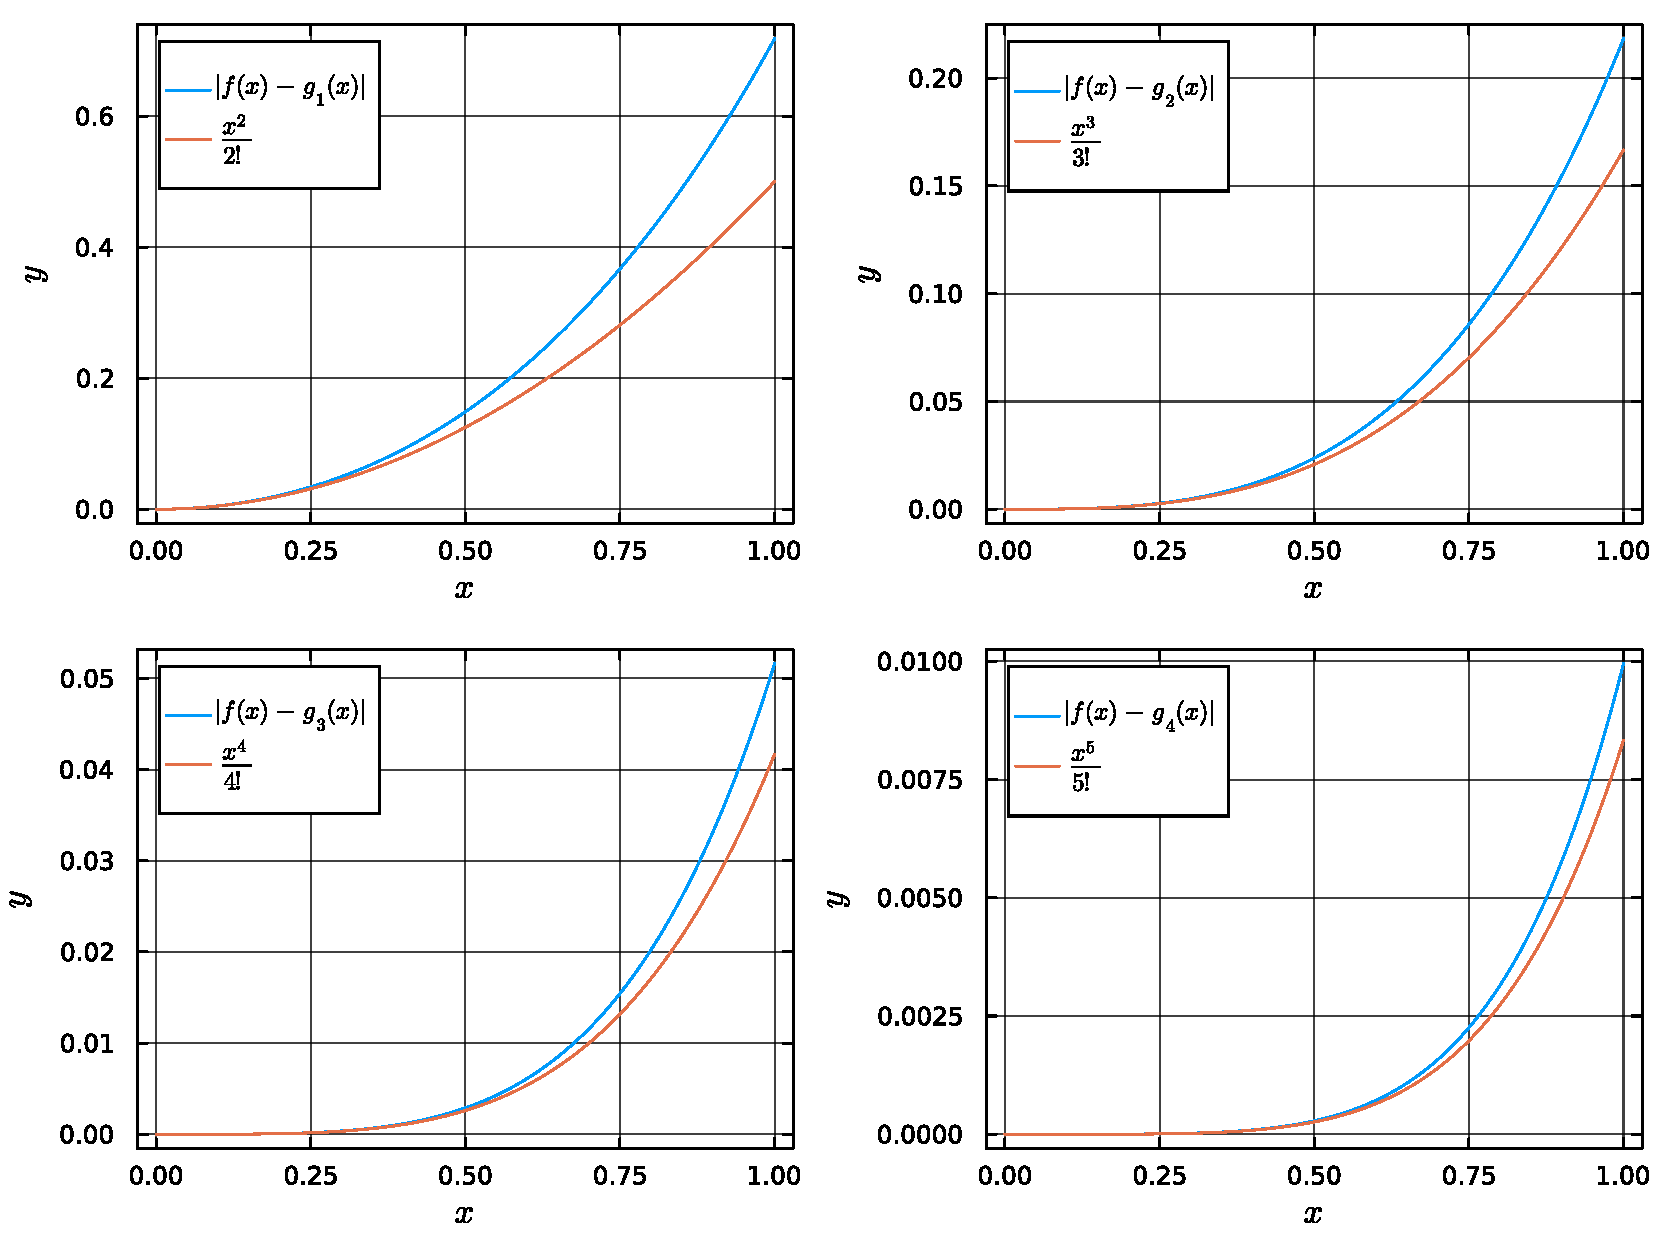
\includegraphics[width=0.8\textwidth]{1011.pdf}
    \caption{Confronto tra $\Delta$ e $\frac{x^{N+1}}{(N+1)!}$ per $N=1,2,3, 4$.}
    \label{fig:es1_0_1_1}
\end{figure}

La prima considerazione che possiamo fare è che all'aumentare di $N$ la funzione $\Delta$ 
assume valori sempre più vicini allo zero. Questo significa che la distanza tra il valore 
della funzione $f(x)$ presa in esame e la sua espansione di Taylor troncata all'ordine 
$N$ diminuisce. In effetti ci aspettiamo che la funzione $\Delta$ sia 
esattamente zero nel caso in cui $N \rightarrow \infty$. Inoltre possiamo notare che la funzione $\Delta$, in ognuno
dei grafici, è tanto più prossima allo zero quanto più ci si avvicina all'origine, poichè l'espansione in serie 
richiede $x \rightarrow 0$.\\
La seconda considerazione è che le funzioni $\Delta$ e $\frac{x^{N+1}}{(N+1)!}$ si 
avvicinano tra loro all'aumentare di $N$. Questo risponde alla richiesta dell'esercizio, 
cioè che l'errore scali come un polinomio di ordine $N+1$. 

\subsection{Esercizio 1.2.1}
Calcolare la seguente somma

\begin{equation}
    \sum_{n=1}^\infty \frac{1}{n^2}=\frac{\pi^2}{6}
    =\lim_{N\to\infty} S(N)
    \quad
    \text{con}
    \quad
    S(N)=\sum_{n=1}^N \frac{1}{n^2}
\end{equation}

\begin{enumerate}
    \item Calcolarla in single precision utilizzando l'ordinamento normale, $n=1,2,3,\ldots,N$.
    \item Calcolarla  in single precision utilizzando l'ordinamento inverso, $n=N,\ldots,2,1$.
    \item Studiare la convergenza di entrambe le implementazioni in funzione di $N$ tracciando il grafico di $|S(N)-\pi^2/6|$.
    \item Ripetere i punti da 1 a 3 utilizzando double precision.
\end{enumerate}

\subsubsection{Soluzione}
Procediamo prendendo in esame i due casi, single precision e double precision.

\paragraph{Single precision:} 

Si riportano in figura \ref{fig:es1_2_1_1} gli errori di troncamento della serie 
$\sum_{n=1}^\infty \frac{1}{n^2}$, laddove $N$ è il troncamento. La somme sono state eseguite
con variabili di tipo Float32 (single precision).

\begin{figure}[!ht]
    \centering
    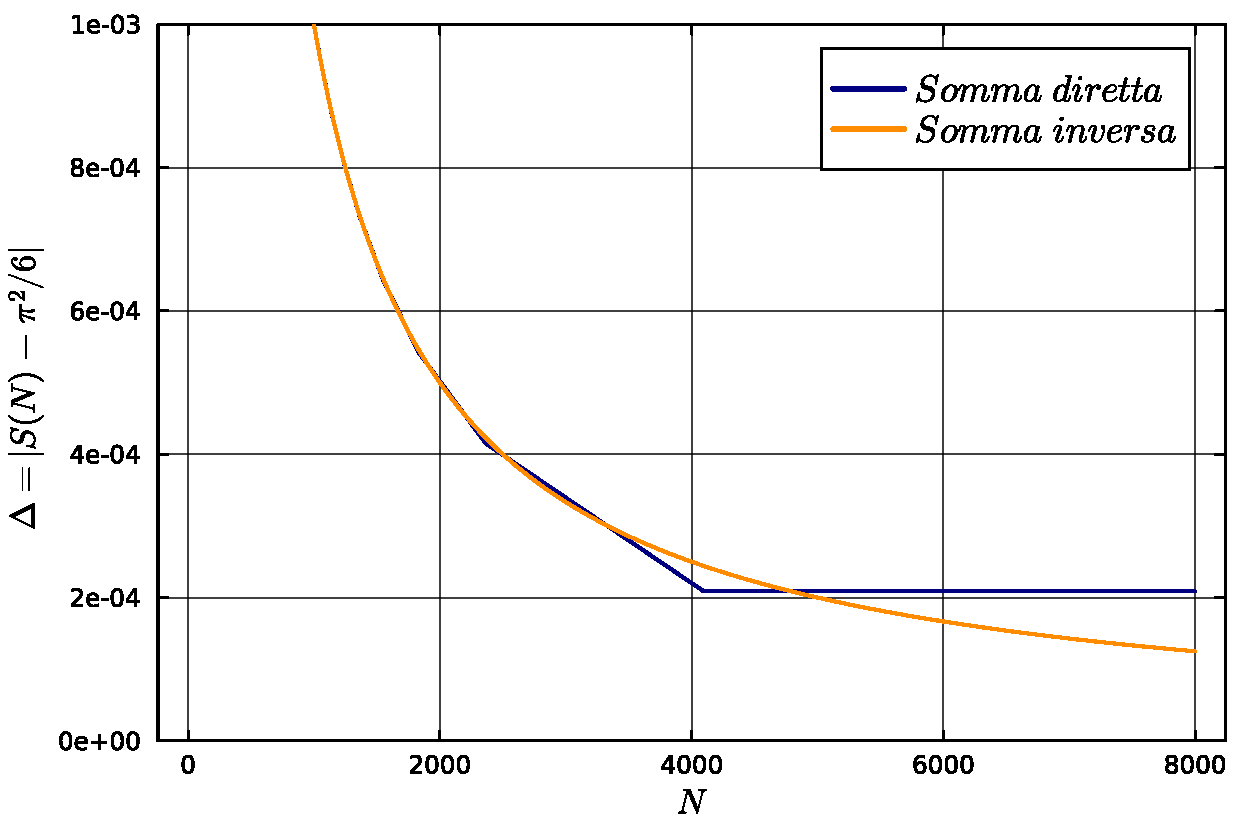
\includegraphics[width=0.8\textwidth]{1211.pdf}
    \caption{$S(N)=\sum_{n=1}^N \frac{1}{n^2}$ in single precision}
    \label{fig:es1_2_1_1}
\end{figure}

In figura \ref{fig:es1_2_1_1} notiamo due comportamenti degni di nota. Il primo riguarda
la curva blu, che arresta la sua discesa poco dopo $N = 4000$. 
Il secondo riguarda il discostarsi delle due curve, già a partire da 
$N \simeq 2000$, a causa dell'andamento a linea spezzata della curva blu.\\
La spiegazione del primo fenomeno è la seguente: nel caso della somma con ordinamento
diretto, all'aumento dell'indice di somma, gli addendi sono sempre più piccoli. In
particolare la somma comincia da 1, e sappiamo che dovrà raggiungere $\frac{\pi^2}{6} \simeq 1.64$ e perciò 
per tutto il processo la somma parziale resterà nell'intervallo $[1, 2)$. In tale intervallo la distanza tra due 
floating point numbers è $\epsilon_{mach} = 2^{-23}$. Osserviamo il grafico \ref{fig:es1_2_1_1}: la curva blu comincia ad essere 
costante a partire da $N = 4096 = 2^{12}$. Tale numero corrisponde all'addendo $\frac{1}{N^2} = 2^{-24}$, 
che è appena più piccolo di $\epsilon_{mach}$, ovvero della distanza tra due floating point numbers in $[1, 2)$, e quindi è
come sommare $0$. \\
La spiegazione del secondo fenomeno è simile: in questo caso alla somma viene aggiunto
un addendo che è più piccolo del precedente, ma non così tanto da essere più piccolo di $\epsilon_{mach}$. In
questo modo la somma viene migliorata, ma il nuovo addendo è arrotondato rispetto al suo valore vero. Il successivo
addendo, pur essendo differente in teoria, a causa dell'arrotondamento risulta essere uguale al precedente. Ciò fa
in modo che venga sommato sempre lo stesso numero, e così l'andamento della curva blu è lineare. \\
I due fenomeni non si verificano per la somma con ordinamento inverso perchè il primo numero ad essere sommato 
è molto piccolo. Questo fa in modo che i successivi floating point number siano molto vicini tra loro, è così sommare
l'addendo successivo fa cadere la somma parziale vicina al floating point number che la approssima. \\
\\
Si può mostrare matematicamente che gli errori $\Delta = |S(N)-\pi^2/6|$ scalano come $O(\frac{1}{N})$. Per verificare questa
affermazione possiamo interpolare la curva degli errori con un metodo che vedremo nella sezione \ref{sistemi_lineari}.
Sulla base delle considerazioni di questa sezione, possiamo aspettarci che sia più conveniente interpolare la curva 
con ordinamento inverso, perchè i valori che la compongono sono meno affetti da errori di tipo numerico. Utilizzando 
il modello linearizzato $log(\Delta) = -c log(N)$ con $c = 1$ si ottiene per l'ordinamento inverso 
$c_{fit} = 1.00003$ e per quello diretto $c_{fit} = 0.986$. Come atteso il caso di ordinamento diretto restituisce un
risultato peggiore di quello inverso.


\paragraph{Double precision:}

Si riporta in figura \ref{fig:es1_2_1_2} un ingrandimento del grafico degli errori di troncamento della serie 
$\sum_{n=1}^\infty \frac{1}{n^2}$, laddove $N$ è il troncamento. La somme sono state eseguite
con variabili di tipo Float64 (double precision).

\begin{figure}[!ht]
    \centering
    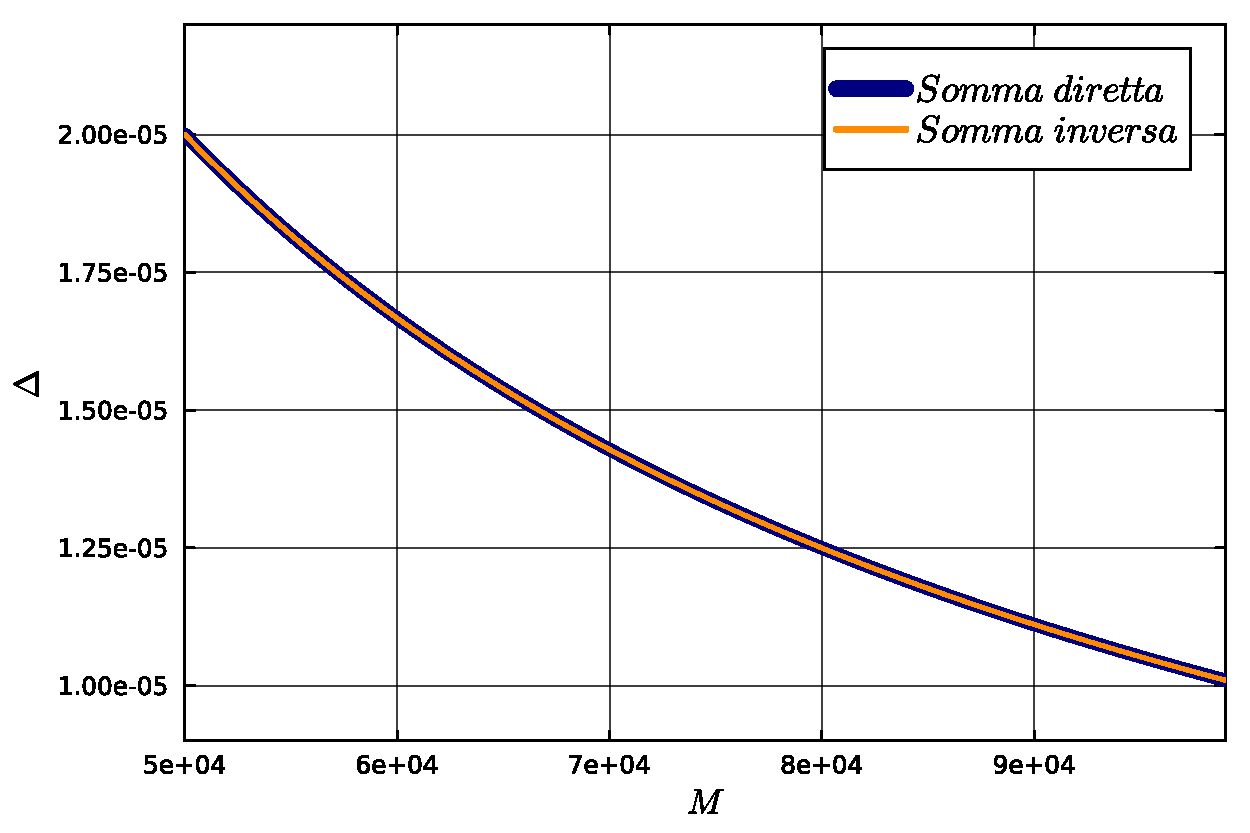
\includegraphics[width=0.8\textwidth]{1212.pdf}
    \caption{Ingrandimento di $S(N)=\sum_{n=1}^N \frac{1}{n^2}$ in double precision}
    \label{fig:es1_2_1_2}
\end{figure}

Nel caso di figura \ref{fig:es1_2_1_2} possiamo notare che le due curve sono sovrapposte, 
nonostante l'ingrandimento a valori di $N \in [5000, 10000]$. Per osservare un fenomeno simile a quello di 
figura \ref{fig:es1_2_1_1} dovremmo raggiungere valori di $N = 2^{26}$. Infatti l'approssimazione non migliora
quando vengono sommati numeri dell'ordine di $\epsilon_{mach}$ per double precision, cioè
 $\frac{1}{N^2} \simeq 2^{-52}$.

\subsection{Esercizio 1.4.1}
\paragraph{(a)} In statistica, definiamo la varianza di un campione di valori $x_1,\ldots,x_n$ come

\begin{equation}
    \sigma^2 = \frac{1}{n-1} \sum_{i=1}^n (x_i - \overline{x})^2,
    \qquad 
    \overline{x} = \frac{1}{n} \sum_{i=1}^n x_i.
    \label{eq:varianza_naive}
\end{equation}

Scrivi una funzione che prenda in input un vettore $x$ di lunghezza arbitraria e restituisca $\sigma^2$ calcolata 
con la formula sopra. 
Dovresti testare la funzione con $x=[1,1,\ldots,1]$ e con alcuni vettori casuali.

\paragraph{(b)} La formula \ref{eq:varianza_naive} ha lo svantaggio di scorrere due volte il vettore dei dati. 
Considera la formula \ref{eq:varianza_eff} a un ciclo:

\begin{equation}
    \sigma^2 = \frac{1}{n-1} \left( u - \frac{1}{n}v^2 \right),\\
    u  = \sum_{i=1}^n x_i^2, 
    \qquad
    v = \sum_{i=1}^n x_i.  
    \label{eq:varianza_eff}  
\end{equation}

Prova entrambe le formule per i seguenti dataset, ciascuno dei quali ha varianza esattamente uguale a 1. 
Esegui i calcoli sia in single che in double precision. 
\begin{align}
    x_1 &= [ 1\cdot 10^3,\ 1+10^3,\ 2+10^3 ] \qquad
    x_2 = [ 1\cdot 10^6,\ 1+10^6,\ 2+10^6 ] \notag \\
    x_3 &= [ 1\cdot 10^7,\ 1+10^7,\ 2+10^7 ] \qquad
    x_4 = [ 1\cdot 10^8,\ 1+10^8,\ 2+10^8 ]
\end{align}


\subsubsection{Soluzione}
\paragraph{(a) } Si è testato il codice che implementa la formula \ref{eq:varianza_naive} su tre vettori contenenti
elementi di tipo Float64. Il primo contiene solo numeri $1$, il secondo contiene numeri generati a partire 
da una distribuzione uniforme, il terzo numeri generati a partiere da una distribuzione normale. I valori sono 
riportati in tabella \ref{tab:varianza_test}.

\begin{table}[!ht]
\centering
\caption{Risultati del test della formula \ref{eq:varianza_naive} su tre vettori di tipo Float64}
\label{tab:varianza_test}
\begin{tabular}{|l|c|c|c|}
\hline
\textbf{Vettore} & \textbf{Lunghezza}   & \textbf{Varianza attesa} & \textbf{Varianza (output)} \\
\hline
Solo uno         & $10^3$               & 0.000                    & 0.000                       \\
Uniforme         & $10^8$               & 0.083                    & 0.083                       \\
Normale          & $10^8$               & 1.000                    & 1.000                       \\
\hline
\end{tabular}
\end{table}

I risultati di tabella \ref{tab:varianza_test} mostrano che l'implementazione del codice è corretta.

\paragraph{(b) }
Si è testato il codice che implementa la formula \ref{eq:varianza_eff} su quattro vettori contenenti
elementi di tipo Float32, Float64 e Long Double. I risultati sono riportati in tabella \ref{tab:varianza_precisioni}.

\begin{table}[!ht]
\centering
\caption{Valori di varianza. Metodo 1: equazione \ref{eq:varianza_naive}. Metodo 2: equazione \ref{eq:varianza_eff}.}
\label{tab:varianza_precisioni}
\begin{tabular}{|l|c|cc|cc|cc|}
\hline
\textbf{Set} & \textbf{$\sigma^2$ attesa} 
& \multicolumn{2}{c|}{\textbf{Float32}} 
& \multicolumn{2}{c|}{\textbf{Float64}} 
& \multicolumn{2}{c|}{\textbf{Long Double}} \\
\cline{3-8}
      &     & Metodo 1 & Metodo 2  & Metodo 1 & Metodo 2 & Metodo 1 & Metodo 2 \\
\hline
$x_1$ & 1.0 & 1.0      & 1.0       & 1.0      & 1.0      & 1.0      & 1.0 \\
$x_2$ & 1.0 & 1.0      & -131072.0 & 1.0      & 1.0      & 1.0      & 1.0 \\
$x_3$ & 1.0 & 1.0      & 0.0       & 1.0      & 1.0      & 1.0      & 1.0 \\
$x_4$ & 1.0 & 0.0      & 0.0       & 1.0      & 0.0      & 1.0      & 1.0 \\
\hline
\end{tabular}
\end{table}

I risultati di tabella \ref{tab:varianza_precisioni} mostrano che il calcolo della varianza con la formula 
\ref{eq:varianza_eff} è più affetto dalla mancanza di precisione della rappresentazione dei numeri durante il calcolo.
Infatti, mano a mano che la la precisione dei numeri aumenta, il risultato della formula \ref{eq:varianza_eff} 
si avvicina a quello atteso. \\
C'è da notare che anche la formula \ref{eq:varianza_naive} è affetta dalla stessa problematica, ma in maniera meno
evidente. Basti osservare il risultato del metodo 1 per il vettore $x_4$ in Float32, che è $0.0$, contro l'atteso 
$1.0$. \\
Parte del problema risiede nella cancellazione numerica. Infatti, per valori degli elementi del vettore molto grandi,
la differenza tra il quadrato della sommma e la somma dei quadrati è molto piccola e incorre in problema di
cancellazione. Per verificare questa affermazione, si riportano in tabella \ref{tab:errore_varianza} i valori della 
differenza \( u - \frac{v^2}{n} \)
per la formula \ref{eq:varianza_eff}.

\begin{table}[!ht]
\centering
\caption{Differenza \( u - \frac{v^2}{n} \) per ciascun dataset.}
\label{tab:errore_varianza}
\begin{tabular}{|l|c|c|c|}
\hline
\textbf{Dataset} & \textbf{Single} & \textbf{Double} & \textbf{Long Double} \\
\hline
$x_1$ & 2.0       & 2.0 & 2.0 \\
$x_2$ & -262144.0 & 2.0 & 2.0 \\
$x_3$ & 0.0       & 2.0 & 2.0 \\
$x_4$ & 0.0       & 0.0 & 2.0 \\
\hline
\end{tabular}
\end{table}

Leggendo la tabella \ref{tab:errore_varianza} possiamo notare che per il dataset $x_1$ la differenza è esattamente
$2.0$, che è il risultato atteso. Per il dataset $x_2$ la differenza è molto grande, $-262144.0$, il che indica un
significativo problema di cancellazione numerica. Per il dataset $x_3$ e $x_4$, la differenza è $0.0$, indice 
del fatto che i singoli valori \( u - \frac{v^2}{n} \) sono vicini tra loro meno di $\epsilon_mach$, e perciò la 
loro differenza è zero. \\
Per concludere, possiamo dire che la formula \ref{eq:varianza_eff} è più efficiente in termini di tempo di calcolo,
ma è più affetta da errori numerici rispetto alla formula \ref{eq:varianza_naive}.

\subsection{Esercizio 1.4.2}
Sia $f(x) = \frac{e^x-1}{x}$.
  
(a) Trova il numero di condizionamento $\kappa_f(x)$. Qual è il massimo di $\kappa_f(x)$ nell'intervallo $-1\le x \le 1$?
  
(b) Usa l'algoritmo "naive"

\begin{equation}
    f(x)= \frac{e^x-1}{x}
    \label{eq:algoritmo_naive}
\end{equation}

per calcolare $f(x)$ per $x=10^{-3},10^{-4},10^{-5},\ldots,10^{-16}$.

(c) Crea un secondo algoritmo utilizzando i primi $n$ termini della serie di Mc Laurin, cioè

\begin{equation}
    p(x) = 1 + \frac{1}{2!}x + \frac{1}{3!}x^2 + \cdots + \frac{1}{(n+1)!}x^n.
    \label{eq:algoritmo_maclaurin}
\end{equation}

Valutalo sugli stessi valori di $x$ del punto (b). Per farlo devi scegliere un valore per $n$. Verifica la stabilità del risultato al variare di $n$. Avresti potuto indovinare un buon valore di $n$ fin dall'inizio?

(d) Confronta i risultati delle due implementazioni in funzione di $x$. Quale algoritmo pensi sia più accurato, e perché?

\subsubsection{Soluzione}

\paragraph{(a) } Il numero di condizionamento di una funzione $f$ è definito come:
\begin{equation}
    \kappa_f(x) = \left| \frac{x f'(x)}{f(x)} \right|\,.
\end{equation}

Per la funzione $f(x) = \frac{e^x-1}{x}$, calcoliamo la derivata:
\begin{equation}
    f'(x) = \frac{e^x x - (e^x - 1)}{x^2} = \frac{e^x (x-1) + 1}{x^2}\,.
\end{equation}
Quindi il numero di condizionamento diventa:
\begin{equation}
    \kappa_f(x) = \left| \frac{x \left( \frac{e^x (x-1) + 1}{x^2} \right)}{\frac{e^x - 1}{x}} \right| = \left| \frac{e^x (x-1) + 1}{(e^x - 1)x} \right| = \left| \frac{e^x x}{(e^x - 1)} - 1 \right|\,.
\end{equation}
La derivata di $k_f(x)$ non si annulla mai nell'intervallo $-1 \leq x \leq 1$, e $\kappa_f(0) = 0$. Dato che
$\kappa_f(x)$ è monotona crescente per $x \geq 0$ e monotona decrescente per $x < 0$, il massimo si ha in $x = 1$,
dove assume il valore $\kappa_f(1) = 0.58198$.

\paragraph{(b)-(c): } Si riportano in figura \ref{fig:es1_4_2_1} i risultati dei due algoritmi. La dicitura $f(x)$ 
si riferisce alla funzione calcolata con l'algoritmo "naive", mentre $p_n(x)$ si riferisce alla funzione calcolata 
con la serie di Maclaurin, fino al termine $n$.

\begin{figure}[!ht]
    \centering
    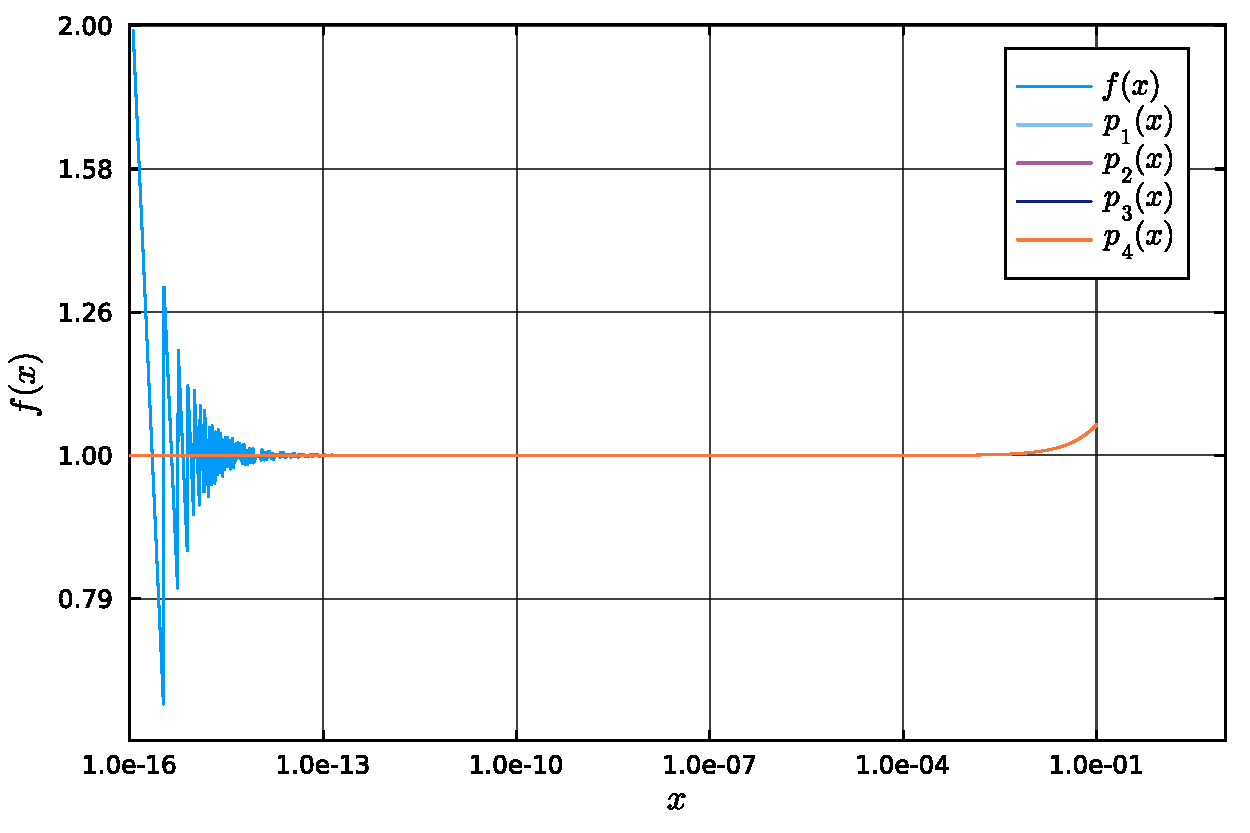
\includegraphics[width=0.8\textwidth]{1421.pdf}
    \caption{Confronto tra $f(x)$ e $p_n(x)$ al variare di $x$.}
    \label{fig:es1_4_2_1}
\end{figure}

Per uno studio più accurato, si riportano nelle figure \ref{fig:es1_4_2_2} e \ref{fig:es1_4_2_3} ingrandimenti 
delle curve di figura \ref{fig:es1_4_2_1}.
\begin{figure}[!ht]
    \centering
    \begin{minipage}[b]{0.49\textwidth}
        \centering
        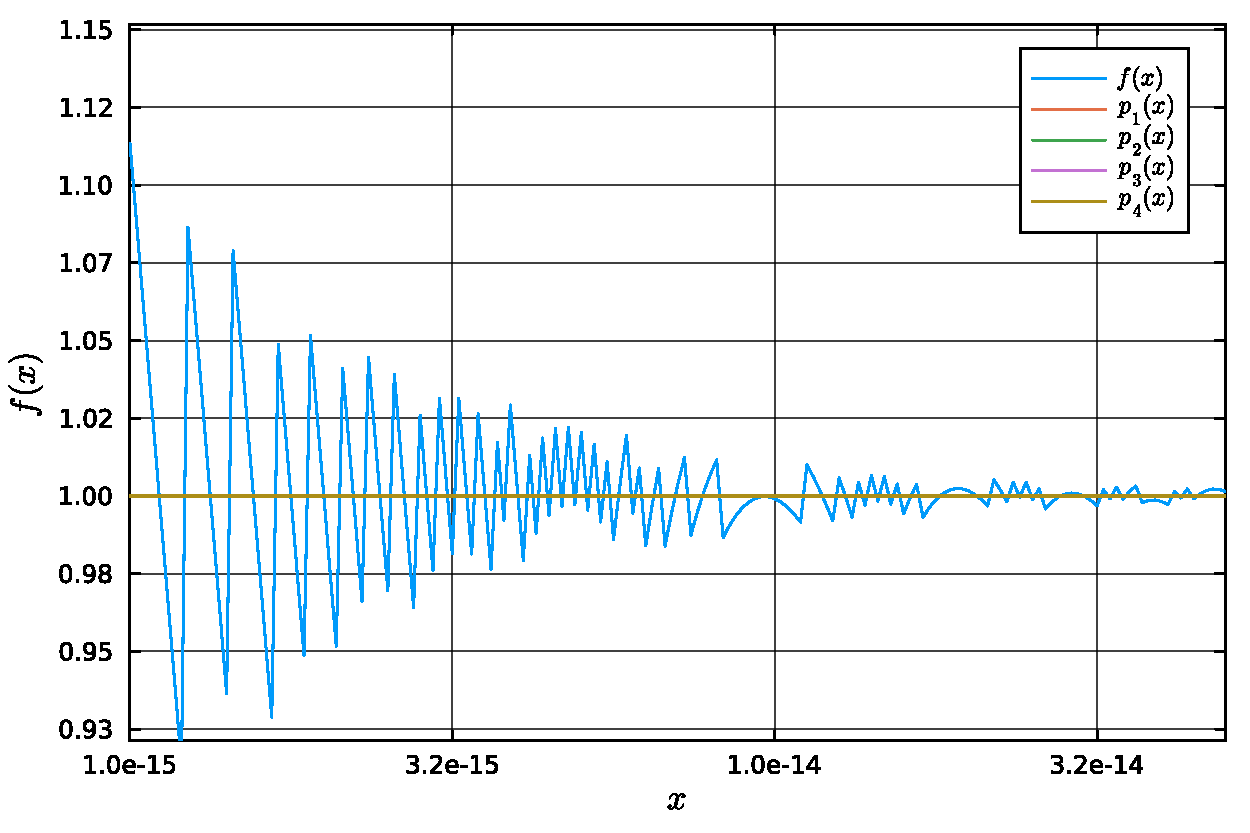
\includegraphics[width=0.8\textwidth]{1422.pdf}
        \caption{Ingrandimento. $x \in [10^{-15}, 10^{-14}]$.}
        \label{fig:es1_4_2_2}
    \end{minipage}
    \hfill
    \begin{minipage}[b]{0.49\textwidth}
        \centering
        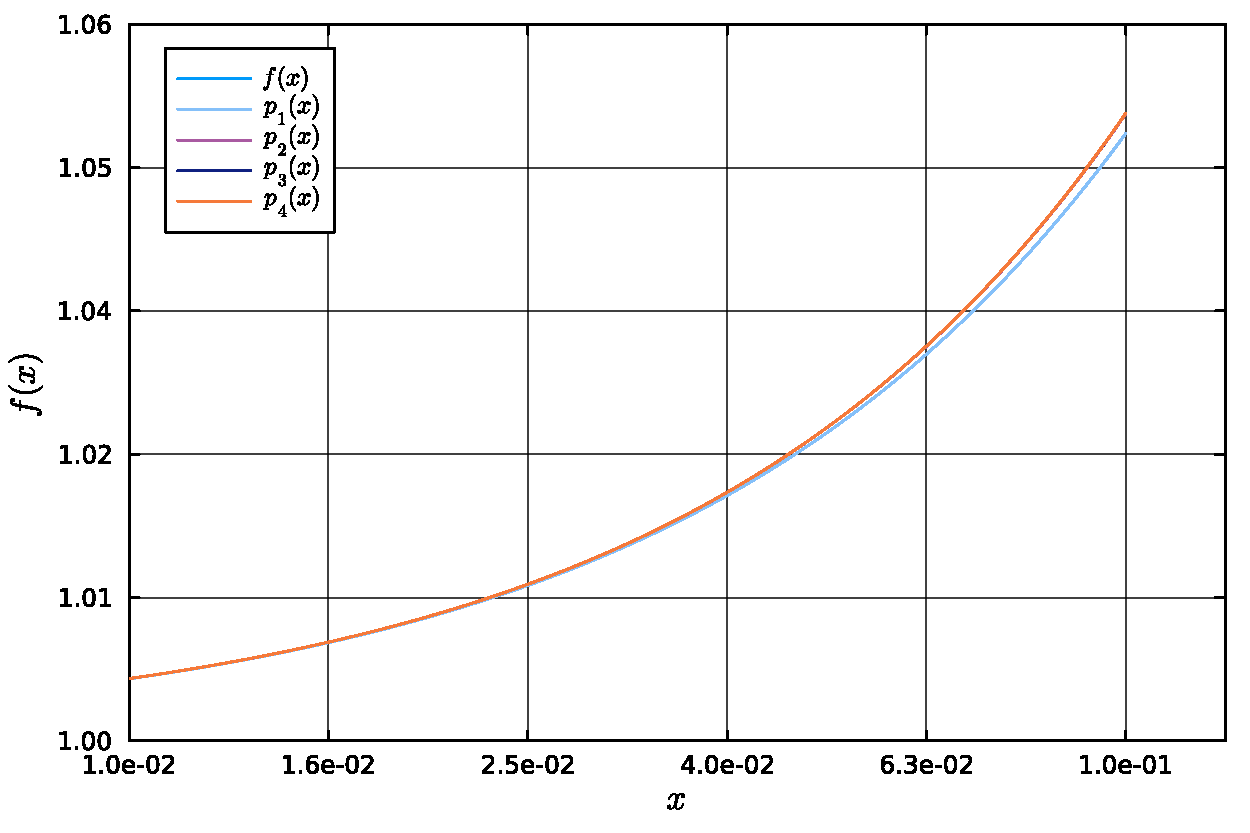
\includegraphics[width=0.8\textwidth]{1423.pdf}
        \caption{Ingrandimento. $x \in [10^{-2}, 10^{-1}]$.}
        \label{fig:es1_4_2_3}
    \end{minipage}
\end{figure}

Per quanto riguarda il comportamento della funzione $f(x)$ calcolata con l'algoritmo \ref{eq:algoritmo_naive},
possiamo notare che per valori di $x$ piccoli la funzione assume valori non corretti, nonostante $\kappa_f(x)$ 
abbia un massimo non molto
grande e peraltro non assunto nell'intorno di zero. La spiegazione di questo fenomeno è che l'algoritmo
\ref{eq:algoritmo_naive}, nonostante non abbia $\kappa_f(x)$ complessivo molto grande, è affetto da errori 
di cancellazione numerica a causa della forma in cui è scritta la funzione, ma non a causa del fatto che 
il problema sia intrinsecamente instabile. Di fatto possiamo intuire che esista una possibile riscrittura
della funzione che non sia affetta da cancellazione numerica, e che sia più stabile, proprio perchè 
sappiamo che il massimo di $\kappa_f(x)$ non è molto grande. Tale riscrittura è quella che utilizza la
serie di Mc Laurin, implementata nell'algoritmo $p_n(x)$. \\
Possiamo notare che l'algoritmo \ref{eq:algoritmo_maclaurin}, per valori di $x$ piccoli, restituisce il 
valore corretto, dato che non è affetto da cancellazione numerica. Al contrario, nella regione ingradita di 
figura \ref{fig:es1_4_2_3}, l'algoritmo \ref{eq:algoritmo_maclaurin} comincia a restituire valori errati
perchè ci allontaniamo dalla regione di convergenza della serie di Mc Laurin. \\
Osservando la figura \ref{fig:es1_4_2_3}, notiamo che, per valori di $x$ fissati, l'algoritmo 
\ref{eq:algoritmo_maclaurin} è stabile, cioè le curve che descrivono i valori di $p_n(x)$ sono sempre più 
vicine tra loro all'aumentare di $n$, fino a sovrapporsi. Per stimare un buon valore di $n$ da utilizzare
per calcolare $p_n(x)$, possiamo osservare che la serie di Mc Laurin è tanto meno stabile quanto più ci si
allontana da zero. Nel caso di studio valutiamo la distanza tra i valori di $p_n(x)$ al variare di $n$,
fissato $x = 0.1$. Si è rappresentato in figura \ref{fig:es1_4_2_4} l'andamento della distanza tra i valori
di $p_n(0.1)$ e $p_{n+1}(0.1)$ al variare di $n$. In formula:
\begin{equation}
    \Delta_n = |p_n(0.1) - p_{n+1}(0.1)|\,.
\end{equation}
\begin{figure}[!ht]
    \centering
    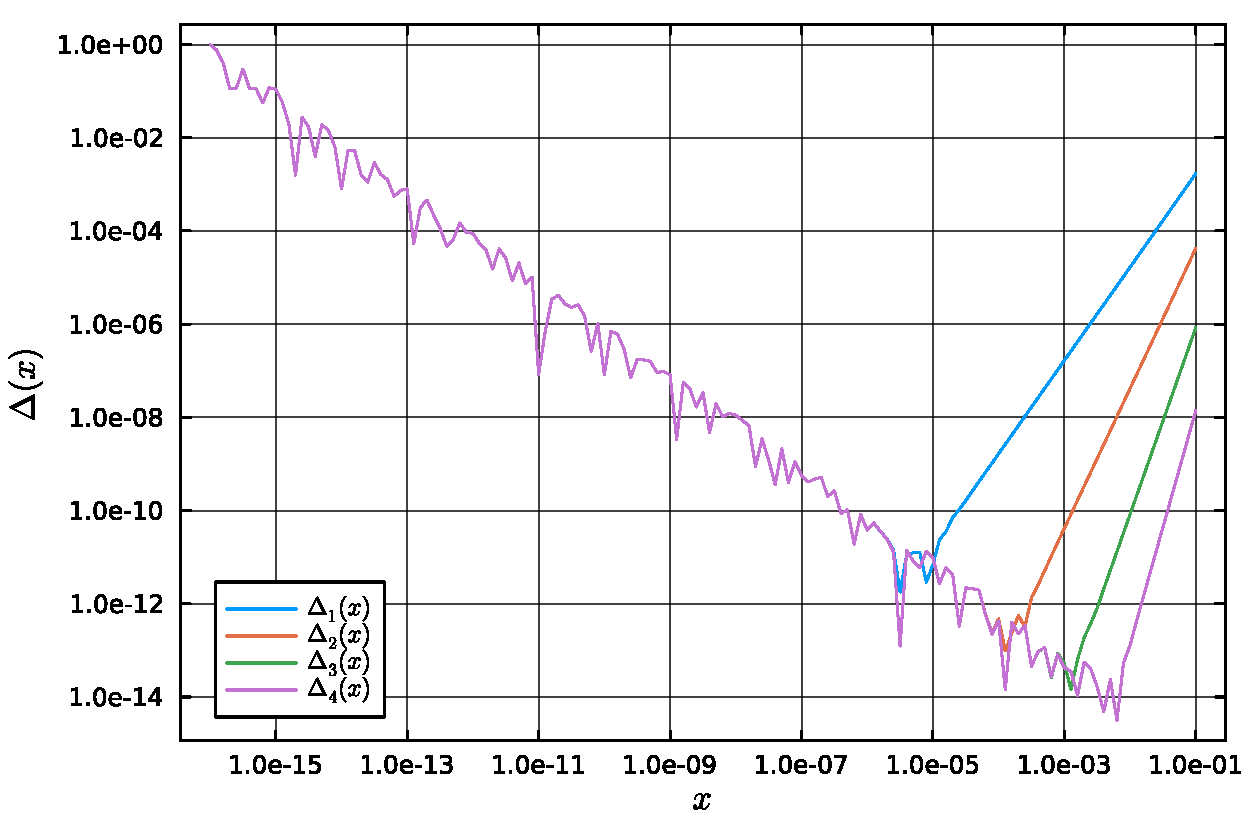
\includegraphics[width=0.8\textwidth]{1424.pdf}
    \caption{Distanza tra $p_n(0.1)$ e $p_{n+1}(0.1)$ al variare di $n$.}
    \label{fig:es1_4_2_4}
\end{figure}

Ai fini di questo esercizio possiamo dire che $n = 2$ è già un buon valore perchè le distanze tra i 
polinomi successivi non sono apprezzabili nel range $[1, 1.06]$, caratteristico della figura \ref{fig:es1_4_2_3}.
È chiaro che volendo raggiungere precisione massima occorrerà scegliere $n = 10$, dato che $\Delta_n$ 
corrispondente è più piccolo di $\epsilon{mach}$

\paragraph{(d): } Come confronto tra i due algoritmi si riporta in figura \ref{fig:es1_4_2_4} il grafico 
dell'errore tra i due algoritmi, cioè
\begin{equation}
    \Delta(x) = \left| f(x) - p_n(x) \right|\,.
\end{equation}

\begin{figure}[!ht]
    \centering
    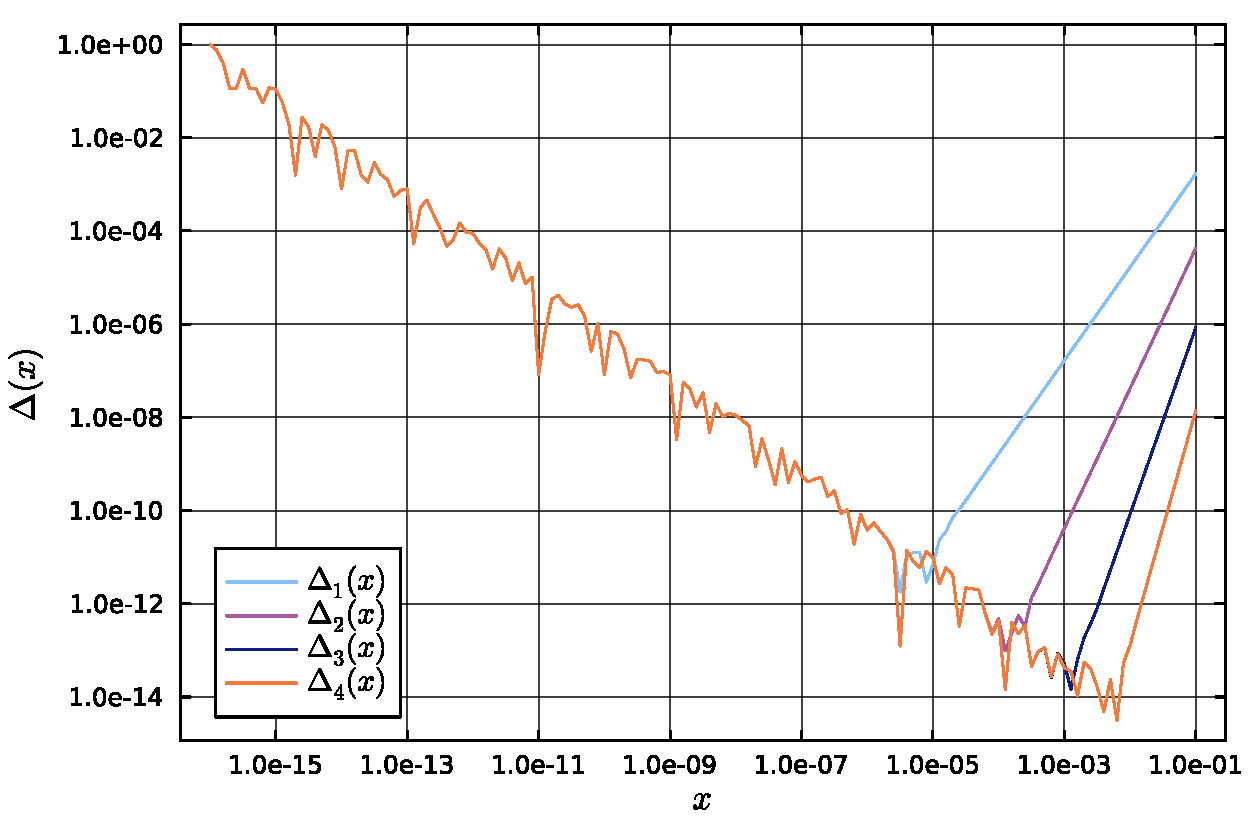
\includegraphics[width=0.8\textwidth]{1425.pdf}
    \caption{Distanza tra $f(x)$ e $p_n(x)$.}
    \label{fig:es1_4_2_5}
\end{figure}

La figura \ref{fig:es1_4_2_5} mostra una evidente differenza tra i due algoritmi nella regione di instabilità
numerica di dell'algoritmo \ref{eq:algoritmo_naive}, cioè per valori di $x$ piccoli. E' interessante notare che 
la distanza tra i due algoritmi diminuisce all'aumentare di $x$, ma torna ad aumentare a partire da
$x = 10^{-5}$, laddove l'algoritmo \ref{eq:algoritmo_maclaurin} esce dalla regione di convergenza della 
serie di Maclaurin. \\
In conclusione, possiamo affermare che l'algoritmo \ref{eq:algoritmo_maclaurin} è più accurato
per valori di $x$ piccoli, mentre l'algoritmo \ref{eq:algoritmo_naive} è più accurato per valori di $x$
grandi.

\section{Sistemi lineari}
\label{sistemi_lineari}
\subsection{Esercizi 2.1.1, 2.1.2, 2.1.3, 2.1.4}
Scrivi una funzione che esegua la sostituzione in avanti su una matrice triangolare inferiore $n\times n$.

2. Testa il tuo codice sui seguenti sistemi lineari:
     
    \begin{minipage}{0.48\textwidth}
        (a) $\; \begin{bmatrix}
            -2 & 0 & 0 \\
            1 & -1 & 0 \\
            3 & 2 & 1 
          \end{bmatrix} 
          \mathbf{x} = \begin{bmatrix}
            -4 \\ 2 \\ 1
          \end{bmatrix}$
    \end{minipage}
    \hfill
    \begin{minipage}{0.48\textwidth}
        (b) $\;\begin{bmatrix}
            4 & 0 & 0 & 0 \\
            1 & -2 & 0 & 0 \\
            -1 & 4 & 4 & 0 \\
            2 & -5 & 5 & 1
          \end{bmatrix} 
          \mathbf{x} = \begin{bmatrix}
            -4 \\ 1 \\ -3 \\ 5
          \end{bmatrix}$
    \end{minipage}

Puoi verificare la soluzione risolvendo il sistema a mano e/o calcolando $\mathbf{L}\mathbf{x} - \mathbf{b}$.

3. Scrivi una funzione che esegua la sostituzione all'indietro su una matrice triangolare superiore $n\times n$.

4. Testa il tuo codice sui seguenti sistemi lineari:

    \begin{minipage}{0.48\textwidth}
        (a) $\;\begin{bmatrix}
            3 & 1 & 0  \\
            0 & -1 & -2  \\
            0 & 0 & 3  \\
            \end{bmatrix} \mathbf{x} = \begin{bmatrix}
            1 \\ 1 \\ 6
            \end{bmatrix}$
    \end{minipage}
    \hfill
    \begin{minipage}{0.48\textwidth}
        (b) $\;\begin{bmatrix}
            3 & 1 & 0 & 6 \\
            0 & -1 & -2 & 7 \\
            0 & 0 & 3 & 4 \\
            0 & 0 & 0 & 5
            \end{bmatrix} \mathbf{x} = \begin{bmatrix}
            4 \\ 1 \\ 1 \\ 5
            \end{bmatrix}$
    \end{minipage}

Puoi verificare la soluzione risolvendo il sistema a mano e/o calcolando $\mathbf{U}\mathbf{x} - \mathbf{b}$.

\subsubsection{Soluzione}
Per risolvere i sistemi lineari proposti, si sono implementate le funzioni di sostituzione in avanti e all'indietro. 
Di seguito sono riportati i risultati delle soluzioni.
\paragraph{Sostituzione in avanti:}
\begin{itemize}
    \item Per il sistema (a) si ha $\mathbf{x} = \begin{bmatrix} -4.0 & 2.0 & 1.0 \end{bmatrix}$.
    \item Per il sistema (b) si ha $\mathbf{x} = \begin{bmatrix} -4.0 & 1.0 & -3.0 & 5.0 \end{bmatrix}$.
\end{itemize}
Risolvendo i sistemi a mano, i valori sono:
\begin{itemize}
    \item Per il sistema (a) si ha $\mathbf{x} = \begin{bmatrix} -4 & 2 & 1 \end{bmatrix}$.
    \item Per il sistema (b) si ha $\mathbf{x} = \begin{bmatrix} -4 & 1 & -3 & 5 \end{bmatrix}$.
\end{itemize}
\paragraph{Sostituzione all'indietro:}
\begin{itemize}
    \item Per il sistema (a) si ha $\mathbf{x} = \begin{bmatrix} 1.0 & 1.0 & 6.0 \end{bmatrix}$.
    \item Per il sistema (b) si ha $\mathbf{x} = \begin{bmatrix} 4.0 & 1.0 & 1.0 & 5.0 \end{bmatrix}$.
\end{itemize}
Risolvendo i sistemi a mano, i valori sono:
\begin{itemize}
    \item Per il sistema (a) si ha $\mathbf{x} = \begin{bmatrix} 1 & 1 & 6 \end{bmatrix}$.
    \item Per il sistema (b) si ha $\mathbf{x} = \begin{bmatrix} 4 & 1 & 1 & 5 \end{bmatrix}$.
\end{itemize}
I risultati confermano la correttezza delle implementazioni delle funzioni di sostituzione in avanti e all'indietro.

\subsection{Esercizi 2.3.1, 2.3.2, 2.3.4}
1. Scrivi una funzione che esegua la fattorizzazione LU di una matrice $n\times n$.

2. Per ciascuna matrice, calcola la fattorizzazione LU e verifica la correttezza.

\begin{center}
    \begin{minipage}{0.32\textwidth}
    \centering
    \[
    \textbf{(A)}\quad
    \begin{bmatrix}
    2 & 3 & 4 \\
    4 & 5 & 10 \\
    4 & 8 & 2
    \end{bmatrix}
    \]
    \end{minipage}
    \hfill
    \begin{minipage}{0.32\textwidth}
    \centering
    \[
    \textbf{(B)}\quad
    \begin{bmatrix}
    6 & -2 & -4 & 4\\
    3 & -3 & -6 & 1 \\
    -12 & 8 & 21 & -8 \\
    -6 & 0 & -10 & 7
    \end{bmatrix}
    \]
    \end{minipage}
    \hfill
    \begin{minipage}{0.32\textwidth}
    \centering
    \[
    \textbf{(C)}\quad
    \begin{bmatrix}
    1 & 4 & 5 & -5 \\
    -1 & 0 & -1 & -5 \\
    1 & 3 & -1 & 2 \\
    1 & -1 & 5 & -1 
    \end{bmatrix}
    \]
    \end{minipage}
\end{center}

4. Calcola il determinante delle matrici dell'Esercizio 2 tramite la fattorizzazione LU.

\subsubsection{Soluzione}
\paragraph{(Punti 1 e 2: )} Si sono implementati gli algoritmi di fattorizzazione LU, e si sono testati 
sui tre sistemi proposti. Le scomposizioni ottenute sono le seguenti: 
\begin{center}
    \[
    \mathbf{L}_A =
    \begin{bmatrix}
    1.0  & 0.0 & 0.0 \\
    2.0  & 1.0 & 0.0 \\
    2.0  & -2.0 & 1.0
    \end{bmatrix}
    \qquad
    \mathbf{U}_A =
    \begin{bmatrix}
    2.0 &  3.0  & 4.0 \\
    0.0  & -1.0  & 2.0 \\
    0.0  & 0.0   & -2.0
    \end{bmatrix}
    \qquad
    \]

    \[
    \mathbf{L}_B =
    \begin{bmatrix}
    1.0  & 0.0   & 0.0  & 0.0 \\
    0.5  & 1.0   & 0.0  & 0.0 \\
    -2.0  & -2.0  & 1.0  & 0.0 \\
    -1.0  & 1.0   & -2.0 & 1.0 \\
    \end{bmatrix}
    \qquad
    \mathbf{U}_B =
    \begin{bmatrix}
    6.0  & -2.0  & -4.0  & 4.0  \\
    0.0  & -2.0  & -4.0  & -1.0 \\
    0.0  & 0.0   & 5.0   & -2.0 \\
    0.0  & 0.0   & 0.0   & 8.0  \\
    \end{bmatrix}
    \qquad
    \]

    \[
    \mathbf{L}_C =
    \begin{bmatrix}
    1.0  & 0.0   & 0.0  & 0.0 \\
    -1.0  & 1.0   & 0.0  & 0.0 \\
    1.0  & -0.25 & 1.0  & 0.0 \\
    1.0  & -1.25 & -1.0 & 1.0 
    \end{bmatrix}
    \qquad
    \mathbf{U}_C =
    \begin{bmatrix}
    1.0  & 4.0   & 5.0  & -5.0 \\
    0.0  & 4.0   & 4.0  & -10.0 \\
    0.0  & 0.0   & -2.0 & 6.0 \\
    0.0  & 0.0   & 0.0  & 2.0 
    \end{bmatrix}
    \qquad
    \]
\end{center}

Per verificare la correttezza delle scomposizioni, si è calcolato il prodotto $\mathbf{L}\mathbf{U}$ per ciascuna 
matrice e lo si è sottratto alla matrice originale. Si sono ottenute matrici di zeri, in tutti i casi, 
confermando la correttezza dell'algoritmo.

\paragraph{(Punto 4: )} Si è calcolato il determinante delle matrici dell'esercizio 2 utilizzando la loro
fattorizzazione LU. Ricordando le proprietà del determinante e che la matrice $\mathbf{L}$ è triangolare inferiore 
con elementi diagonali unitari, si ha che:

\begin{equation}
    \det(\mathbf{M}) = det(\mathbf{LU}) = \det(\mathbf{L}) \cdot \det(\mathbf{U}) = \det(\mathbf{U})\,.
\end{equation}

Per il calcolo del determinante delle matrici proposte si è eseguito il prodotto degli elementi della diagonale
principale della matrice $\mathbf{U}$. A titolo di confronto si è calcolato il determinante delle matrici con 
la funzione \texttt{det} di Julia. I risultati sono riportati in tabella \ref{tab:determinanti}.
\begin{table}[!ht]
\centering
\caption{Determinanti delle matrici dell'esercizio 2.}
\label{tab:determinanti}
\begin{tabular}{|l|c|c|}
\hline
\textbf{Matrice} & \textbf{Determinante (LU)} & \textbf{Determinante (Julia)} \\
\hline
A                & 4.0                        & 4.0 \\
B                & -480.0                     & -480.0 \\
C                & 80.0                       & 80.0  \\
\hline
\end{tabular}
\end{table}

Si ottengono risultati identici.

\subsection{Esercizio 2.3.3}
Le matrici
\[
\mathbf{T}(x,y) = \begin{bmatrix}
    1 & 0 & x \\ 
    0 & 1 & y \\ 
    0 & 0 & 1
\end{bmatrix},\qquad
\mathbf{R}(\theta) = \begin{bmatrix}
    \cos\theta & \sin \theta & 0 \\ 
    -\sin\theta & \cos \theta & 0 \\
    0 & 0 & 1
\end{bmatrix}
\]
sono usate per rappresentare traslazioni e rotazioni di punti del piano in computer grafica. Per quanto segue, sia
\[
\mathbf{A} = \mathbf{T}(3,-1)\,\mathbf{R}(\pi/5)\,\mathbf{T}(-3,1), \qquad 
\mathbf{z} = \begin{bmatrix}
    2 \\ 2 \\ 1
\end{bmatrix}.
\]

\begin{enumerate}
        \item[(a)] Calcolare $\mathbf{b} = \mathbf{A}\mathbf{z}$.
        \item[(b)] Trovare la fattorizzazione LU di $\mathbf{A}$.
        \item[(c)] Usare i fattori e le sostituzioni triangolari per risolvere $\mathbf{A}\mathbf{x} = \mathbf{b}$ 
                   e calcolare $\mathbf{x} - \mathbf{z}$.
\end{enumerate}

\subsubsection{Soluzione}
\paragraph{(a) } Si calcola il prodotto tra le matrici $\mathbf{A}$ e $\mathbf{z}$, ottenendo:
\begin{equation}
    \mathbf{b} = \mathbf{A}\mathbf{z} = \begin{bmatrix}
        3.95 \\
        2.01 \\
        1.0
    \end{bmatrix}. 
\end{equation}
\paragraph{(b) } Si calcola la fattorizzazione LU della matrice $\mathbf{A}$, ottenendo:
\begin{equation}
    \mathbf{L} = \begin{bmatrix}
        1.0  &     0.0  & 0.0 \\
        -0.8  &  1.0  & 0.0 \\
        0.0  &  0.0  &  1.0
    \end{bmatrix}, \qquad
    \mathbf{U} = \begin{bmatrix}
        0.81  &  0.59  &  1.16 \\
        0.0       &  1.24   &  2.42 \\
        0.0       &  0.0       &  1.0
    \end{bmatrix}.
\end{equation}
\paragraph{(c) } Si risolve il sistema $\mathbf{A}\mathbf{x} = \mathbf{b}$ utilizzando le sostituzioni triangolari.
Si ottiene, con le dovute approssimazioni:
\begin{equation}
    \mathbf{x} = \begin{bmatrix}
        2.0 \\ 
        2.0 \\ 
        1.0
    \end{bmatrix},
    \qquad
    \mathbf{x} - \mathbf{z} = \begin{bmatrix}
        -2.22 \cdot 10^{-16}  \\
        -4.44 \cdot 10^{-16}  \\
        0.0
    \end{bmatrix}.
\end{equation}

\subsection{Esercizi 2.4.1, 2.4.2}
1. Scrivi un programma che esegua la decomposizione di Cholesky di una matrice $n\times n$. \\
2. Per ciascuna matrice, utilizza la decomposizione di Cholesky per determinare se è definita positiva.

\begin{center}
    \begin{minipage}{0.32\textwidth}
    \centering
    \[
    \mathbf{A} =
    \begin{bmatrix}
    1 & 0 & -1 \\
    0 & 4 & 5 \\
    -1 & 5 & 10
    \end{bmatrix}
    \]
    \end{minipage}
    \hfill
    \begin{minipage}{0.32\textwidth}
    \centering
    \[
    \mathbf{B} =
    \begin{bmatrix}
    1 & 0 & 1 \\
    0 & 4 & 5 \\
    1 & 5 & 10
    \end{bmatrix}
    \]
    \end{minipage}
    \hfill
    \begin{minipage}{0.32\textwidth}
    \centering
    \[
    \mathbf{C} =
    \begin{bmatrix}
    1 & 0 & 1 \\
    0 & 4 & 5 \\
    1 & 5 & 1
    \end{bmatrix}
    \]
    \end{minipage}
\end{center}

\begin{center}
    \begin{minipage}{0.48\textwidth}
    \centering
    \[
    \mathbf{D} =
    \begin{bmatrix}
    6 & 2 & 1 & 0 \\
    2 & 6 & 2 & 1 \\
    1 & 2 & 5 & 2 \\
    0 & 1 & 2 & 4
    \end{bmatrix}
    \]
    \end{minipage}
    \hfill
    \begin{minipage}{0.48\textwidth}
    \centering
    \[
    \mathbf{E} =
    \begin{bmatrix}
    4 & 1 & 2 & 7 \\
    1 & 1 & 3 & 1 \\
    2 & 3 & 5 & 3 \\
    7 & 1 & 3 & 1
    \end{bmatrix}
    \]
    \end{minipage}
\end{center}

\subsubsection{Soluzione}
Si è implementato l'algoritmo di decomposizione di Cholesky, e si sono testate le matrici proposte. L'algoritmo
è giunto a conclusione per le matrici $\mathbf{A}$, $\mathbf{B}$ e $\mathbf{D}$, ma ha restituito un messaggio di
errore per le matrici $\mathbf{C}$ e $\mathbf{E}$, indicando che non sono definite positive. 
Si riportano i risultati delle decomposizioni giunte a termine, con i dovuti arrotondamenti. 

\begin{center}
    \begin{minipage}{0.32\textwidth}
    \centering
    \[
    \mathbf{R_A} =
    \begin{bmatrix}
        1.0  &  0.0  &  -1.0 \\
        0.0  &  2.0  &  2.5 \\
        0.0  &  0.0  &  1.7
    \end{bmatrix}
    \]
    \end{minipage}
    \hfill
    \begin{minipage}{0.32\textwidth}
    \centering
    \[
    \mathbf{R_B} =
    \begin{bmatrix}
    1.0  &  0.0  &  1.0 \\
    0.0  &  2.0  &  2.5 \\
    0.0  &  0.0  &  1.7
    \end{bmatrix}
    \]
    \end{minipage}
    \hfill
    \begin{minipage}{0.32\textwidth}
    \centering
    \[
    \mathbf{R_D} =
    \begin{bmatrix}
    2.45 & 0.82 & 0.41 & 0.00 \\
    0.00 & 2.29 & 0.73 & 0.41 \\
    0.00 & 0.00 & 2.06 & 0.82 \\
    0.00 & 0.00 & 0.00 & 1.84
    \end{bmatrix}
    \]
    \end{minipage}
\end{center}

\subsection{Esercizio 2.5.1}
Consideriamo la matrice:
\[
\mathbf{A} =
\begin{bmatrix}
-\epsilon &  1 \\
        1 & -1
\end{bmatrix}
\]

Se $\epsilon=0$, la fattorizzazione LU senza pivoting parziale fallisce per $\mathbf{A}$. Ma se $\epsilon\neq 0$, 
possiamo procedere senza pivoting, almeno in linea di principio. \\
(a) Costruisci $\mathbf{b}=\mathbf{Ax}$ prendendo $\epsilon=10^{-12}$ per la matrice $\mathbf{A}$ e 
$\mathbf{x}=[1,1]$ come soluzione. \\
(b) Fattorizza la matrice usando la decomposizione LU senza pivoting e risolvi numericamente per $\mathbf{x}$. 
Quanto è accurato il risultato? \\
(c) Verifica la fattorizzazione LU calcolando $\mathbf{A}-\mathbf{LU}$. Funziona? \\
(d) Ripeti per $\epsilon=10^{-20}$. Quanto è accurato ora il risultato? \\
(e) Calcola il numero di condizionamento della matrice $\mathbf{A}$; puoi scegliere la norma che preferisci. 
Il sistema $\mathbf{Ax}=\mathbf{b}$ è mal condizionato? \\
(f) Calcola le matrici $\mathbf{L}$ e $\mathbf{U}$ della fattorizzazione LU di $\mathbf{A}=\mathbf{LU}$ a mano. \\
(g) Calcola i numeri di condizionamento di $\mathbf{L}$ e $\mathbf{U}$. 

\subsubsection{Soluzione}
Per poter operare un confronto tra i risultati ottenuti con $\epsilon = 10^{-12}$ e $\epsilon = 10^{-20}$, si è
scelto di trattare il punto (d) insieme ai punti (a), (b) e (c). Il pedice 1 è legato al caso $\epsilon = 10^{-12}$,
il pedice 2 al caso $\epsilon = 10^{-20}$. \\

\paragraph{(a) } Si è calcolato il prodotto tra la matrice $\mathbf{A}$ e il vettore $\mathbf{x}$, ottenendo, 
a meno di arrotondamenti, i vettori:
\begin{equation}
    \mathbf{b_1} = \begin{bmatrix}
         1.0 \\
         0.0
    \end{bmatrix}.
\qquad
    \mathbf{b_2} = \begin{bmatrix}
         1.0\\
         0.0
    \end{bmatrix}.
\end{equation}

\paragraph{(b) } \label{par:fattorizzazione_LU} Si è calcolata la fattorizzazione LU della matrice $\mathbf{A}$, 
ottenendo:
\begin{equation}
    \mathbf{L_1} = \begin{bmatrix}
    1.0      &  0.0 \\
    -1.0 \cdot 10^{12}  &  1.0 
    \end{bmatrix}, \qquad
    \mathbf{U_1} = \begin{bmatrix}
    -1.0 \cdot 10^{-12}  &  1.0               \\
     0.0                 &  1.0 \cdot 10^{12}
    \end{bmatrix},
\end{equation}
\begin{equation}
    \mathbf{L_2} = \begin{bmatrix}
    1.0                 &  0.0 \\
    -1.0 \cdot 10^{20}  &  1.0
    \end{bmatrix}, \qquad
    \mathbf{U_2} = \begin{bmatrix}
    -1.0 \cdot 10^{-20}  &  1.0 \\
     0.0                 &  1.0 \cdot 10^{20}
    \end{bmatrix}.
\end{equation}

Si è risolto il sistema $\mathbf{Ax} = \mathbf{b}$ utilizzando le sostituzioni triangolari, ottenendo:
\begin{equation}
    \mathbf{x_1} = \begin{bmatrix}
        1.0 \\
        1.0
    \end{bmatrix}, 
    \qquad
    \mathbf{x_2} = \begin{bmatrix}
        0.0 \\
        1.0
    \end{bmatrix}.
\end{equation}

\paragraph{(c) } Si è calcolato il prodotto tra le matrici $\mathbf{L}$ e $\mathbf{U}$, in seguito lo si è 
sottratto ad $\mathbf{A}$ ottenendo:
\begin{equation}
    \mathbf{A_1} - \mathbf{(LU)_1} = \begin{bmatrix}
        0.0 & 0.0 \\
        0.0 & 0.0
    \end{bmatrix}, 
    \qquad
    \mathbf{A_2} - \mathbf{(LU)_2} = \begin{bmatrix}
        0.0 & 0.0 \\
        0.0 & 1.0
    \end{bmatrix}.
\end{equation}

È evidente che il risultato per $\epsilon = 10^{-12}$ è accurato, al contrario del risultato ottenuto per
$\epsilon = 10^{-20}$, in cui sia la soluzione che la verifica della fattorizzazione LU sono
affette da errori numerici.

\paragraph{(e) } Si è calcolato $\kappa(A)$, utilizzando sia la norma 1 che la norma infinito, ottenendo lo stesso
numero a causa della natura simmetrica della matrice $\mathbf{A}$. La formula generale per il numero di
condizionamento della matrice $\mathbf{A}$ presa in esame è $ \kappa(A) = \frac{4}{1 - \epsilon}$.
\begin{equation}
    \kappa_1(A) = \kappa_\infty(A) =  4.000000000004\,,
    \qquad
    \kappa_1(A) = \kappa_\infty(A) =  4.0\,.
\end{equation}

Come si può notare, in entrambi i casi il numero di condizionamento non è molto grande, quindi il sistema
$\mathbf{Ax} = \mathbf{b}$ non è mal condizionato. 

\paragraph{(f) } Si sono calcolate a mano le matrici $\mathbf{L}$ e $\mathbf{U}$ della fattorizzazione LU di
$\mathbf{A}$ per ciascun valore di $\epsilon$. I calcoli dettagliati sono disponibili nella cartella git,
nel percorso \\ \verb|lab\computazionale1\esercizi\pen_and_paper|. Ad ogni modo le
matrici ottenute sono già state riportate al punto \ref{par:fattorizzazione_LU}. 

\paragraph{(g) } Si sono calcolati i numeri di condizionamento di $\mathbf{L}$ e $\mathbf{U}$, utilizzando sia 
la norma 1 che la norma infinito, ancora una volta ottenendo lo stesso numero. \\
Le forumle generali per il numero di condizionamento delle matrici $\mathbf{L}$ e $\mathbf{U}$ sono:
\begin{equation}
    \kappa_1(L) = \kappa_\infty(L) = \left(1 + \frac{1}{\epsilon}\right)^2\,,
    \qquad
    \kappa_1(U) = \kappa_\infty(U) = \frac{1}{\epsilon^2}\,.
\end{equation}

In tabella \ref{tab:LU_epsilon} sono riassunti i risultati ottenuti.

\begin{table}[!ht]
\centering
\caption{Valori dei parametri \( L \) e \( U \) per diverse tolleranze \( \varepsilon \)}
\label{tab:LU_epsilon}
\begin{tabular}{|c|c|c|}
\hline
 & \( \varepsilon = 10^{-12} \) & \( \varepsilon = 10^{-20} \) \\
\hline
\( L \) & $1.0 \cdot 10^{24}$ & $1.0 \cdot 10^{40}$ \\
\( U \) & $1.0 \cdot 10^{24}$ & $1.0 \cdot 10^{40}$ \\
\hline
\end{tabular}
\end{table}

\subsubsection{Conclusioni}
L'esercizio ha mostrato come il numero di condizionamento di una matrice non sia un indicatore sufficiente per
valutare l'esattezza della risoluzione del sistema lineare associato. Infatti, sebbene il numero di condizionamento
della matrice $\mathbf{A}$ sia relativamente basso, la risoluzione del sistema richiede il calcolo delle matrici
$\mathbf{L}$ e $\mathbf{U}$, il cui numero di condizionamento potrebbe risultare elevato. È questo il caso
con $\epsilon = 10^{-20}$, in cui $\kappa(A) =  4.0$ ma $\kappa(L) = 1.0 \cdot 10^{40}$ e 
$\kappa(U) = 1.0 \cdot 10^{40}$. Dato che l'algoritmo utilizza le matrici $\mathbf{L}$ e $\mathbf{U}$ 
per risolvere il sistema è evidente che l'errore numerico aumenta a causa delle stesse.

\subsection{Esercizio 2.6.1}
(a) Scrivi un programma che prenda in input una matrice $\mathbf{A}$ e un vettore $\mathbf{b}$ e risolva 
il problema dei minimi quadrati $\text{argmin}\| \mathbf{b}- \mathbf{A} \mathbf{x}\|_2$ utilizzando la decomposizione di Cholesky.\\
(b) Per verificare il funzionamento del tuo codice, calcola la soluzione ai minimi quadrati quando
\begin{center}
    \begin{minipage}{0.48\textwidth}
    \centering
    \[
    \mathbf{A} = \begin{bmatrix}
      2 & -1 \\
      0 & 1 \\
      -2 & 2
    \end{bmatrix}, \qquad
    \mathbf{b} = \begin{bmatrix}
      1 \\ -5 \\ 6
    \end{bmatrix}
    \]
    \end{minipage}
\end{center}

\subsubsection{Soluzione}
Si è implementato l'algoritmo per il metodo dei minimi quadrati e lo si è testato sulle matrici proposte, 
ottenendo:
\begin{equation}
    \mathbf{x} = \begin{bmatrix}
        -2.0 \\
        -1.0
    \end{bmatrix}.
\end{equation}

\subsection{Esercizio 2.6.2}
Keplero ha scoperto che il periodo orbitale $\tau$ di un pianeta dipende dalla sua distanza media $R$ dal Sole 
secondo la legge $\tau = c R^{\alpha}$, dove $\alpha$ è un semplice numero razionale. \\
(a) Esegui un fit lineare ai minimi quadrati utilizzando la tabella \ref{tab:pianeti} per determinare il valore 
più probabile e semplice di $\alpha$. \\
(b) Realizza un grafico dei dati e del risultato del fit.

\subsubsection{Soluzione}
\paragraph{(a) } Il metodo dei minimi quadrati che è stato sviluppato durante il corso è adatto a risolvere
problemi lineari, in cui le costanti che si vogliono determinare sono coefficienti lineari di funzioni dei dati.
Non è il caso del problema proposto, dato che $\alpha$ si trova ad esponente. Per risolvere la questione si 
è scelto di linearizzare il problema tramite il logaritmo naturale. In formule:
\begin{equation}
    \ln(\tau) = \ln(c) + \alpha \ln(R).
\end{equation}
Da qui in poi si è implementato il metodo dei minimi quadrati, applicando la scomposizione di Cholesky alla 
matrice $n \times n$ ottenuta dal prodotto della matrice di design e la sua trasposta. Per chiarezza si riporta
la matrice di design trasposta:
\begin{equation}
    \mathbf{A}^T = \begin{bmatrix}
        1 & 1 & \cdots & 1 \\
        \ln(57.59) & \ln(108.11) & \cdots & \ln(4499.9)
    \end{bmatrix}.
\end{equation}

La matrice di regressione è stata costruita in modo che la prima colonna fosse composta da 1, per poter calcolare
il termine noto della retta, e la seconda colonna fosse composta dai logaritmi naturali delle
distanze dei pianeti dal Sole. \\
La legge di Keplero prevista è la seguente:
\begin{equation}
    \label{eq:keplero}
    \tau = c R^{3/2}\,, \text{ con } \qquad \alpha = \frac{3}{2}\, \qquad c = \frac{2\pi}{\sqrt{G (M+m)}}
\end{equation}
dove $G$ è la costante di gravitazione universale, $M$ è la massa del Sole, $m$ è la massa del pianeta. \\
La regressione lineare che si vuole effetturare considera $c$ costante, nonostante dipenda dalla massa del pianeta.
Consideriamo Giove, il pianeta più massivo di quelli presi in esame ($m \approx 1.90 \cdot 10^{27} \, \text{kg}$). Si ha:
\begin{align}
    c_1 &= \frac{2\pi}{\sqrt{G (M+m)}} = 5.47 \cdot 10^{-10} \frac{\text{sec}}{m^{3/2}} = 0.203 \frac{days}{Mkm^{3/2}}  \\
    c_2 &= \frac{2\pi}{\sqrt{G M}}   = 5.47 \cdot 10^{-10} \frac{\text{sec}}{m^{3/2}} = 0.203 \frac{days}{Mkm^{3/2}}    \\
    \frac{c_1}{c_2} &\approx 1.0
\end{align}
Possiamo quindi affermare che la costante $c$ è indipendente dalla massa del pianeta, entro la precisione 
necessaria per il nostro scopo. \\
Si sono quindi stimati il valore di $\alpha$ e della costante $c$, tramite la regressione, ottenendo:
\begin{equation}
    c = 0.206 \frac{days}{Mkm^{3/2}}
    \qquad
    \alpha = 1.499
\end{equation}
I risultati sono in accordo con quanto atteso.

\paragraph{(b) } Si riporta in figura \ref{fig:es2_6_2_1} il grafico dei dati e relativo fit.

\begin{figure}[!ht]
    \centering
    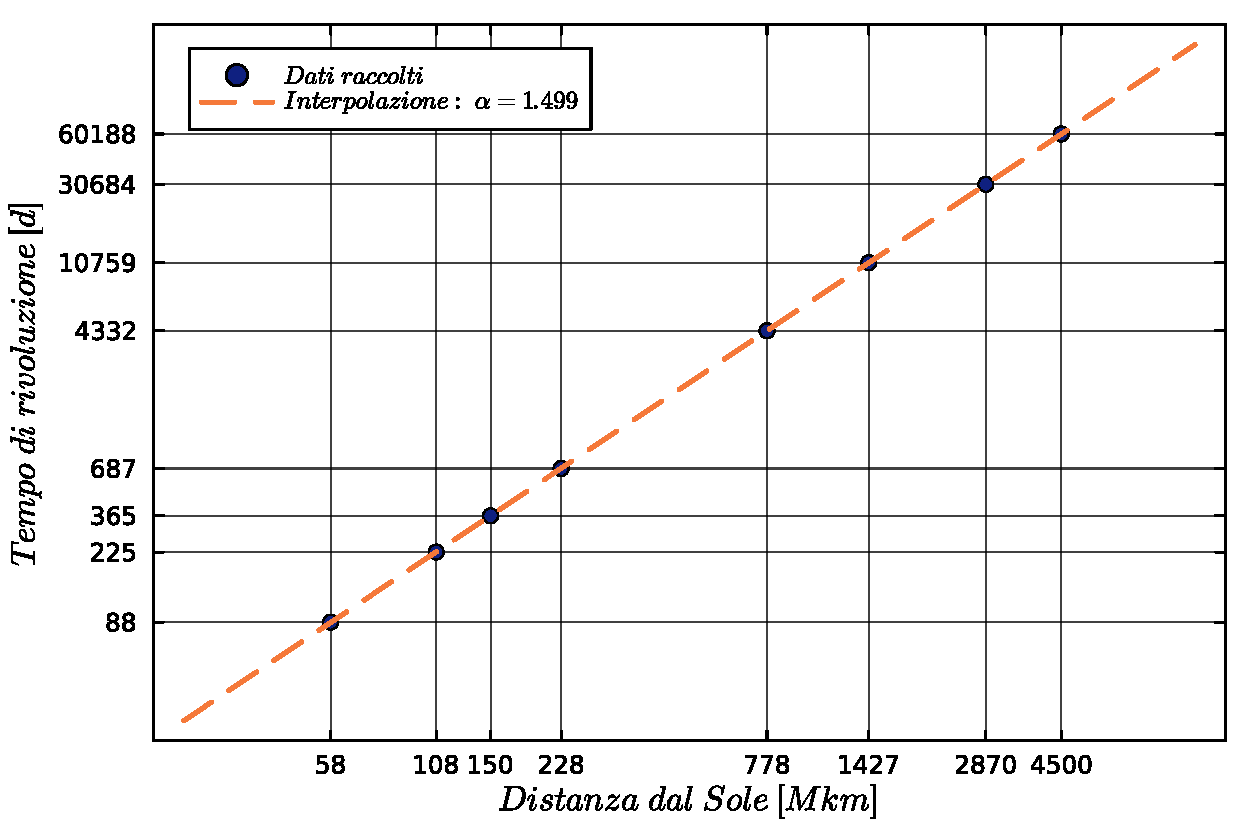
\includegraphics[width=0.8\textwidth]{2621.pdf}
    \caption{Fit lineare ai minimi quadrati dei dati dei pianeti del Sistema Solare.}
    \label{fig:es2_6_2_1}
\end{figure}

\subsection{Esercizio 2.6.3}
In questo esercizio si vuole trovare un'approssimazione della funzione periodica $g(t)=e^{\sin(t-1)}$ su un 
periodo, $0 < t \le 2\pi$. Come dati, si definiscono

\begin{equation}
    t_i = \frac{2\pi i}{60}\,,
    \quad  
    y_i = g(t_i)\,,
    \quad i=1,\ldots,60.
\end{equation}
    
(a) Trova i coefficienti del fit ai minimi quadrati    
    \begin{equation}
    \label{eq:fit_pol}    
        y(t) \approx c_1 + c_2 t + \cdots + c_7 t^6.
    \end{equation}        
Sovrapponi un grafico dei valori dei dati come punti con una curva che mostra il fit. \\
(b) Trova i coefficienti del fit ai minimi quadrati
    \begin{equation}
    \label{eq:fit_fourier}
        y \approx d_1 + d_2\cos(t) + d_3\sin(t) + d_4\cos(2t) + d_5\sin(2t).
    \end{equation}

A differenza del punto (a), questa funzione di fitting è essa stessa periodica. 
Sovrapponi un grafico dei valori dei dati come punti con una curva che mostra il fit.

\subsubsection{Soluzione}
Dopo avere generato i dati richiesti, si è eseguito il metodo dei minimi quadrati con le seguenti 
matrici di regressione:

\begin{equation}
    \mathbf{D_{pol}} = \begin{bmatrix}
        1 & t_1 & \hdots & t_1^6 \\
        1 & t_2 & \hdots & t_2^6 \\
        \vdots & \vdots & \ddots& \vdots \\
        1 & t_{60} & \hdots & t_{60}^6
    \end{bmatrix},
    \qquad
    \mathbf{D_{Four}} = \begin{bmatrix}
        1 & \cos(t_1) & \sin(t_1) & \cos(2t_1) & \sin(2t_1) \\
        1 & \cos(t_2) & \sin(t_2) & \cos(2t_2) & \sin(2t_2) \\
        \vdots & \vdots & \vdots & \vdots & \vdots \\
        1 & \cos(t_{60}) & \sin(t_{60}) & \cos(2t_{60}) & \sin(2t_{60})
    \end{bmatrix},
\end{equation}

ottenendo i coefficienti delle formule \ref{eq:fit_pol} e \ref{eq:fit_fourier}:
\begin{itemize}
    \item Coefficienti del polinomio: $[0.712; -1.351; 2.225; -0.538; -0.074; 0.033; -0.003]$
    \item Coefficienti della funzione di Fourier: $[1.266; -0.951; 0.611; 0.113; -0.247]$
\end{itemize}

Si riportano i grafici dei dati e dei fit in figura \ref{fig:es2_6_3_1}.
\begin{figure}[!ht]
    \centering
    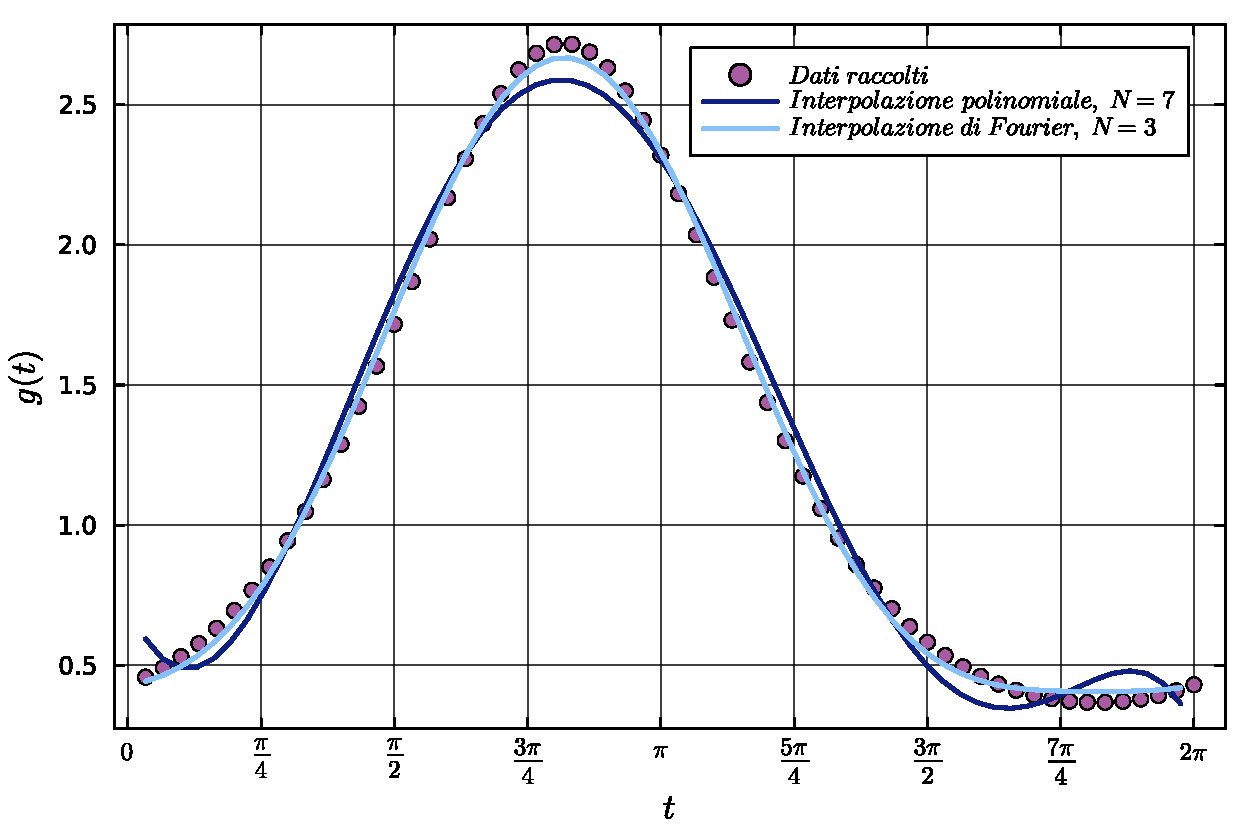
\includegraphics[width=0.8\textwidth]{2631.pdf}
    \caption{Fit polinomiale e di Fourier ai minimi quadrati della funzione $g(t)=e^{\sin(t-1)}$.}
    \label{fig:es2_6_3_1}
\end{figure}

\subsubsection{Conclusioni}
In figura \ref{fig:es2_6_3_1} si osserva che il fit meglio riuscito è quello di Fourier, nonostante
richieda meno parametri. Il motivo è che la funzione $g(t)$ è periodica, e quindi il fit con il modello 
\ref{eq:fit_fourier} riesce a catturare meglio la periodicità della funzione rispetto al fit esguito con 
\ref{eq:fit_pol}. \\
In un contesto sperimentale la funzione $g(t)$ non è nota a priori, anzi lo scopo dell'esperimento è 
solitamente quello di risalire a tale funzione. Il fatto che il fit secondo il modello di Fourier riesca meglio
è indice della natura periodica del fenomeno osservato. 

\section{Radici di equazioni non lineari}
\subsection{Esercizi 3.2.1, 3.2.2}
1. Implementa il metodo di bisezione e testalo con una funzione semplice, ad esempio $f(x)=x$. \\
2. (a) Usa il metodo di bisezione per trovare le soluzioni di $x^3 - 7x^2 + 14x - 6 = 0$ su $[0,1]$.\\
   (b) Studia la convergenza del metodo di bisezione rispetto alla radice trovata in (a). 
   (Puoi prendere come approssimazione per la radice $r=m_{n_{\rm max}}$, dove $n_{\rm max}$ è 
   l'indice corrispondente all'ultima iterazione di bisezione.) \\
   Qual è il suo ordine di convergenza $q$? Puoi stimare la costante d'errore asintotica $C$? \\
   Suggerimento: Studia $d_n=-\log_{10}|x_{n}-r|$ come funzione di $n$.

%Riguarda i conti teorici. Sono giusti ma vanno formalizzati
\subsubsection{Soluzione}
\paragraph{(1) } Si è implementato il metodo di bisezione, e si è testato con la funzione $f(x)=x$ per due 
intervalli: $[-1.0, 1.0]$ e $[-5.0, 1.0]$. Il motivo della scelta di questi due intervalli è che ci aspettiamo che
il metodo restituisca $x = 0$ come soluzione e nel caso di intervallo simmetrico il numero di iterazioni 
è pari ad 1. Con un intervallo asimmetrico il test è più efficiente perchè il numero di iterazioni aumenta. \\
Il metodo si interrompe quando la distanza tra gli estremi risulta minore di $\max(|a|,|b|) \cdot 10^{-16}$,
dove $a$ e $b$ sono gli estremi dell'intervallo. Il metodo ha prodotto i seguenti risultati:
\begin{itemize}
    \item Intervallo $[-1.0, 1.0]$: $x = 0.0$ in 1 iterazione.
    \item Intervallo $[-5.0, 1.0]$: $x = 1.1 \cdot 10^{-162}$ in 539 iterazioni.
\end{itemize}

\paragraph{(2a) } Si è implementato il metodo di bisezione per la funzione $f(x) = x^3 - 7x^2 + 14x - 6$. \\
Il metodo ha restituito un valore della radice $r = 0.5857864376269051$ con $f(r) = 0.0$, in $50$ iterazioni. In
figura \ref{fig:es3_2_2_1} si riporta il grafico della funzione e delle radici successive trovate.
\begin{figure}[!ht]
    \centering
    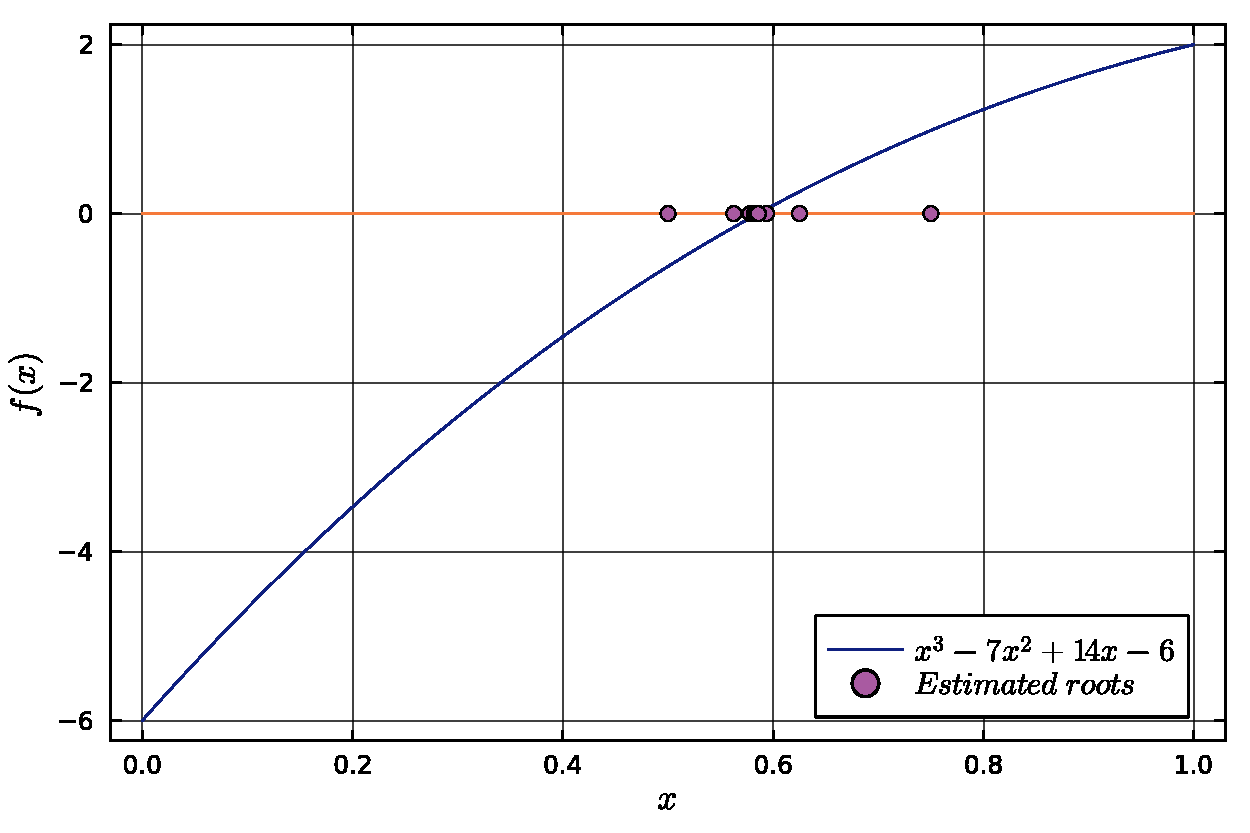
\includegraphics[width=0.8\textwidth]{3221.pdf}
    \caption{Grafico della funzione $f(x) = x^3 - 7x^2 + 14x - 6$ e della radice trovata con il metodo di bisezione.}
    \label{fig:es3_2_2_1}
\end{figure} 

\paragraph{(2b) } Per studiare la convergenza del metodo di bisezione bisogna fare alcune considerazioni 
preliminari. \\
È noto che per il metodo di bisezione vale la relazione $ |m_n-r|< 2^{-(n+1)} (b_0-a_0) $, dove $m_n$ è 
la stima della radice al passo $n$, $r$ è la radice cercata, $a_0$ e $b_0$ sono gli estremi dell'intervallo 
iniziale. \\
Ad ogni iterazione l'intervallo viene dimezzato, in modo che al passo successivo la stima della radice si trovi
in una delle due metà dell'intervallo nella quale si trovava la stima precedente. In formule: 
$|m_{n+1}-r| <\frac{|m_n-r|}{2}$. \\
Unendo le due relazioni presentate sopra si ricava $\frac{|m_{n+1}-r|}{|m_n-r|} < \frac{1}{2}$, e passando al 
limite: 
\begin{equation}
    \label{eq:convergenza_bisezione}
    \lim_{n\to\infty} \frac{|m_{n+1}-r|}{|m_n-r|} = \frac{1}{2}, 
\end{equation}
da cui si ottiene che $q$, ordine di convergenza, 
è 1, mentre C, la costante di errore asintotico, vale $\frac{1}{2}$. \\
Verifichiamolo numericamente, ricordando le relazioni: 

Per verificare i valori teorici di $q$ e $C$ è necessario tenere a mente le seguenti relazioni. La prima si ottiene
applicando il logaritmo decimale alla \ref{eq:convergenza_bisezione}:
\begin{equation}
    \label{eq:convergenza_bisezione_log}
    d_{n+1} \approx q\, d_n - \log_{10}|C|
    \quad\Rightarrow\quad
    \frac{d_{n+1}}{d_n} \approx q - \frac{\log_{10}|C|}{d_n}
    \overset{n\to\infty}{\longrightarrow} q
\end{equation}

dove $d_n = -\log_{10}|m_n - r|$. \\
La seconda si ottiene iterando la relazione  $ |x_{k+1} - r|= C |x_{k} - r|$:
\begin{equation}
    |x_{k+1} - r|= C^{k+1} |x_{0} - r|
\end{equation}

\subparagraph{Stima di $q$ e $C$} Per stimare $q$ si è calcolato il rapporto tra i valori di $d_n$ e $d_{n+1}$ e lo si
è messo in grafico in funzione di $n$, ottenendo la figura \ref{fig:es3_2_2_2}, in cui è presente un ingrandimento
per i valori più alti di n.
\begin{figure}[!ht]
    \begin{minipage}[b]{0.54\textwidth}
    \centering
    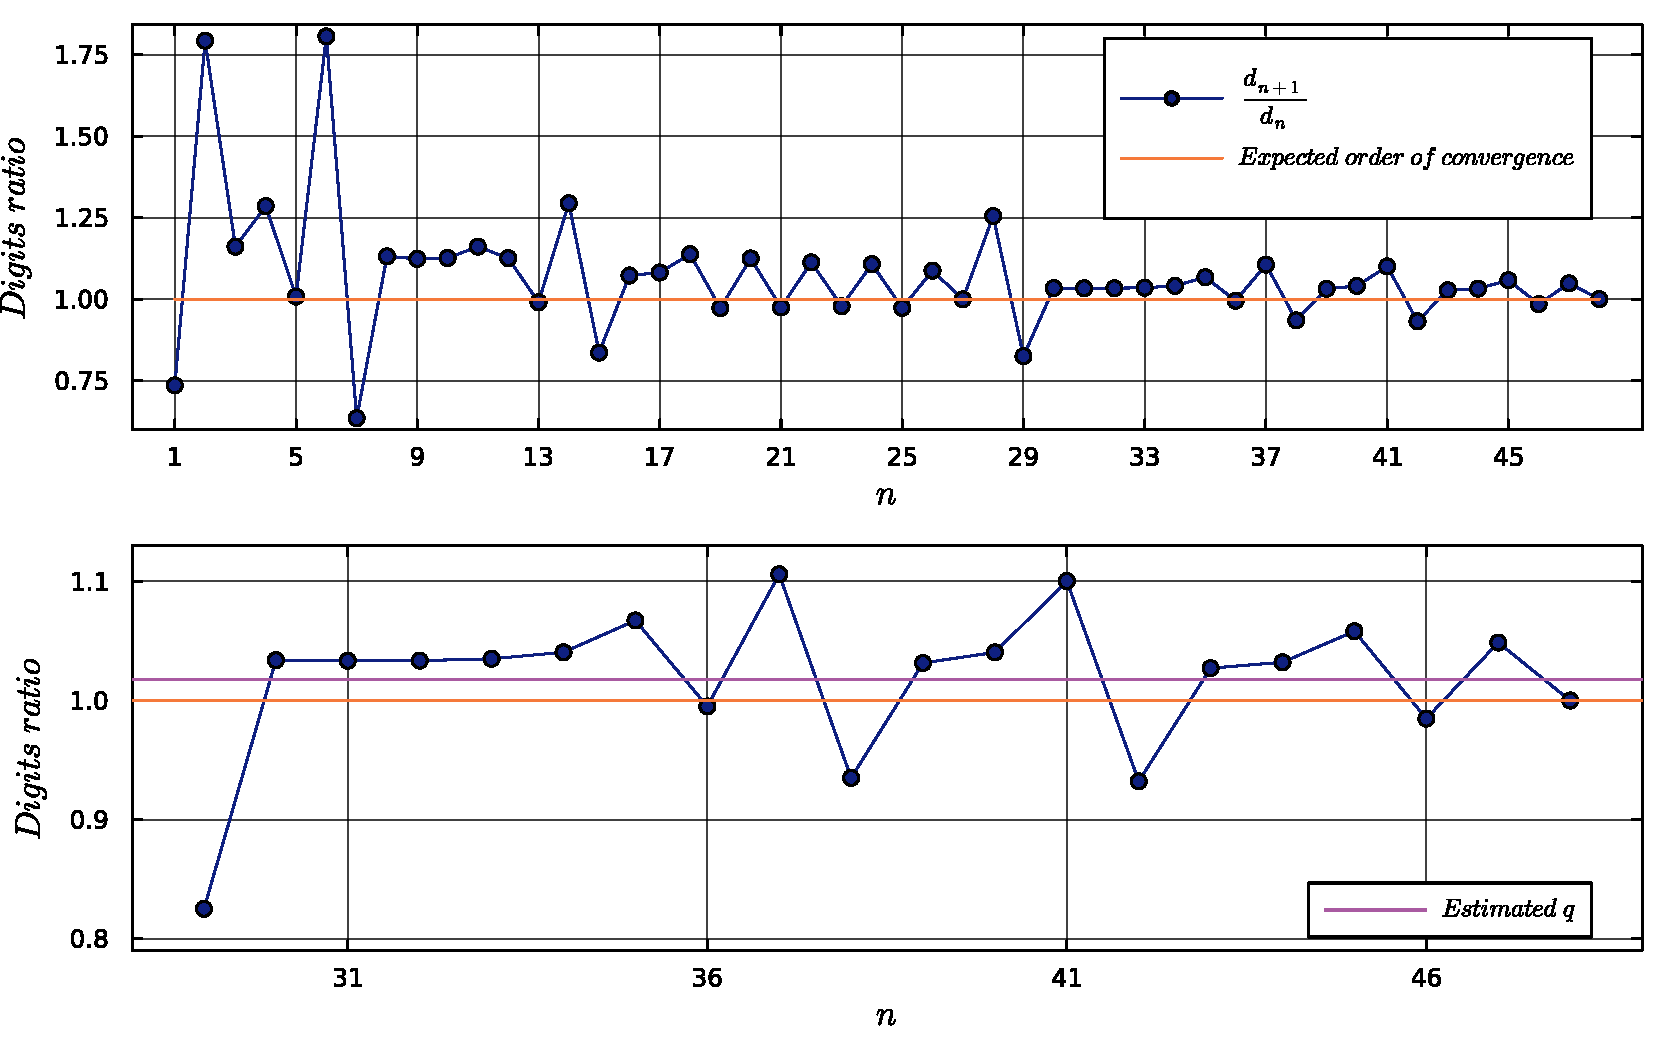
\includegraphics[width=0.8\textwidth]{3222.pdf}
    \caption{Stima di $q$}
    \label{fig:es3_2_2_2}
    \end{minipage}
    \begin{minipage}[b]{0.54\textwidth}
    \centering
    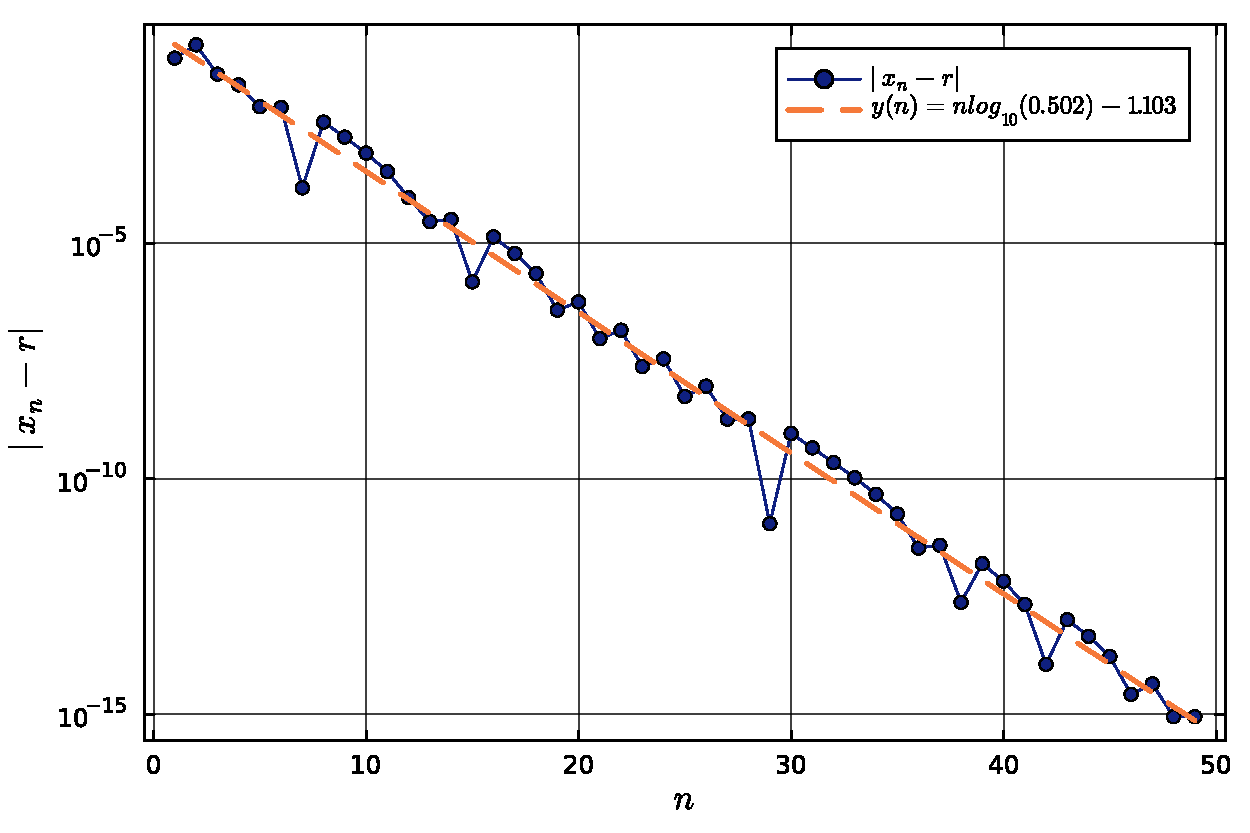
\includegraphics[width=0.8\textwidth]{3223.pdf}
    \caption{Stima di $C$}
    \label{fig:es3_2_2_3}
    \end{minipage}
\end{figure}

Il rapporto tende a 1, come atteso. Si vuole ora quantificare tale valore. \\
La relazione \ref{eq:convergenza_bisezione_log} vale per $n\to\infty$. Ciò significa che la stima di $q$
dovrebbe essere calcolata per l'$n$ più grande possibile. Ciononostante si
è deciso di stimare il valore di $q$ tramite l'interpolazione con funzione costante perchè il valore di $q$ 
fluttua attorno a 1, ed è possibile che per $n$ maggiori di quelli disponibili il valore cercato continui a 
fluttuare attorno a 1. Per l'interpolazione si sono considerati gli ultimi 20 punti della serie, riportati 
nell'ingrandimento di \ref{fig:es3_2_2_2}. Il fit su tali punti restituisce
un valore di $q = 1.02$. \\  

Per stimare $C$ si è eseguito il fit con metodo dei minimi quadrati sul modello:
\begin{equation}
    log |x_{k+1}-r| = (k+1)log(C) + log|x_0 - r|   \rightarrow   y(x) = x log(C) + A ,
\end{equation}
avendo considerato $r$ come l'ultimo valore di $m_n$ calcolato. Si riporta il grafico del fit in 
figura \ref{fig:es3_2_2_3}. \\

Il fit ha restituito i seguenti valori:
\begin{equation}
    C = 0.5,
    \qquad
    A = -0.1.
\end{equation}
Si osserva che il valore di $C$ è in accordo con quanto atteso, mentre il valore di $A$ non è significativo.

\subparagraph{Commento: } È possibile stimare i valori di $q$ e $C$ anche in modo diverso, e con un solo fit.
Interpolando la relazione \ref{eq:convergenza_bisezione_log} con un'iperbole, e ignorando il limite, 
si riescono a ottenere i valori di $q$ e $C$ in un colpo solo. I risultati ottenuti hanno una precisione minore 
di quelli ottenuti  con i metodi precedenti, pertanto non sono riportati. Si rimanda alla cartella git
\verb|lab\computazionale1\esercizi\3_2_2.ipynb| per i dettagli.

\subsection{Esercizi 3.3.1, 3.3.2}
1. Scrivi un programma che implementi il metodo di Newton.\\
2. Per ciascuna delle seguenti funzioni, esegui i seguenti passi.\\  
(a) Riscrivi l'equazione nella forma standard per la ricerca degli zeri, $f(x) = 0$, e calcola $f'(x)$. \\
(b) Traccia il grafico di $f$ nell'intervallo indicato e determina quante radici sono presenti nell'intervallo. \\
(c) Usa il metodo di Newton per trovare ciascuna radice. \\
(d) Studia l'errore nella sequenza di Newton per determinare numericamente se la convergenza è approssimativamente quadratica per la radice trovata. \\
Suggerimento: Studia $d_{n+1}/d_{n}$ con $d_n=-\log_{10}|x_n-r|$ per verificare il tasso di convergenza $q$. Una volta stabilito, prova a stimare la costante d'errore asintotica $C$. \\
\begin{itemize}
    \item $x^2=e^{-x}$, su $[-2,2]$ \\
    \item $2x = \tan x$, su $[-0.2,1.4]$ \\
    \item $e^{x+1}=2+x$, su $[-2,2]$ \\
\end{itemize}
    
\subsubsection{Soluzione}
\paragraph{(1) } Si è implementato il metodo di Newton, e si è testato con la funzione $f(x)=e^x - 1$ con valore
iniziale $x_0 = 10$. Il metodo ha restituito il valore $-6.68 \cdot 10^{-17}$ in 16 iterazioni. 
Valore atteso: $x = 0$. \\

\paragraph{(2a) }\label{sec:332_2a} Le funzioni in forma di ricerca degli zeri sono:
\begin{itemize}
    \item $f_1(x) = x^2 - e^{-x}$, con $f_1'(x) = 2x + e^{-x}$, su $[-2,2]$.
    \item $f_2(x) = 2x - \tan x$, con $f_2'(x) = 2 - \tan^2 x$, su $[-0.2,1.4]$.
    \item $f_3(x) = e^{x+1} - 2 - x$, con $f_3'(x) = e^{x+1} - 1$, su $[-2,2]$.
\end{itemize}

\paragraph{(2b) }\label{sec:332_2b} I grafici delle funzioni sono riportati in figura \ref{fig:es3_3_2_1}, da cui si evince che:
\begin{itemize}
    \item $f_1$ ha una radice nell'intervallo $[-2,2]$.
    \item $f_2$ ha due radici nell'intervallo $[-0.2,1.4]$.
    \item $f_3$ ha una radice nell'intervallo $[-2,2]$.
\end{itemize}

\begin{figure}[!ht]
    \centering
    \begin{minipage}[b]{0.47\textwidth}
        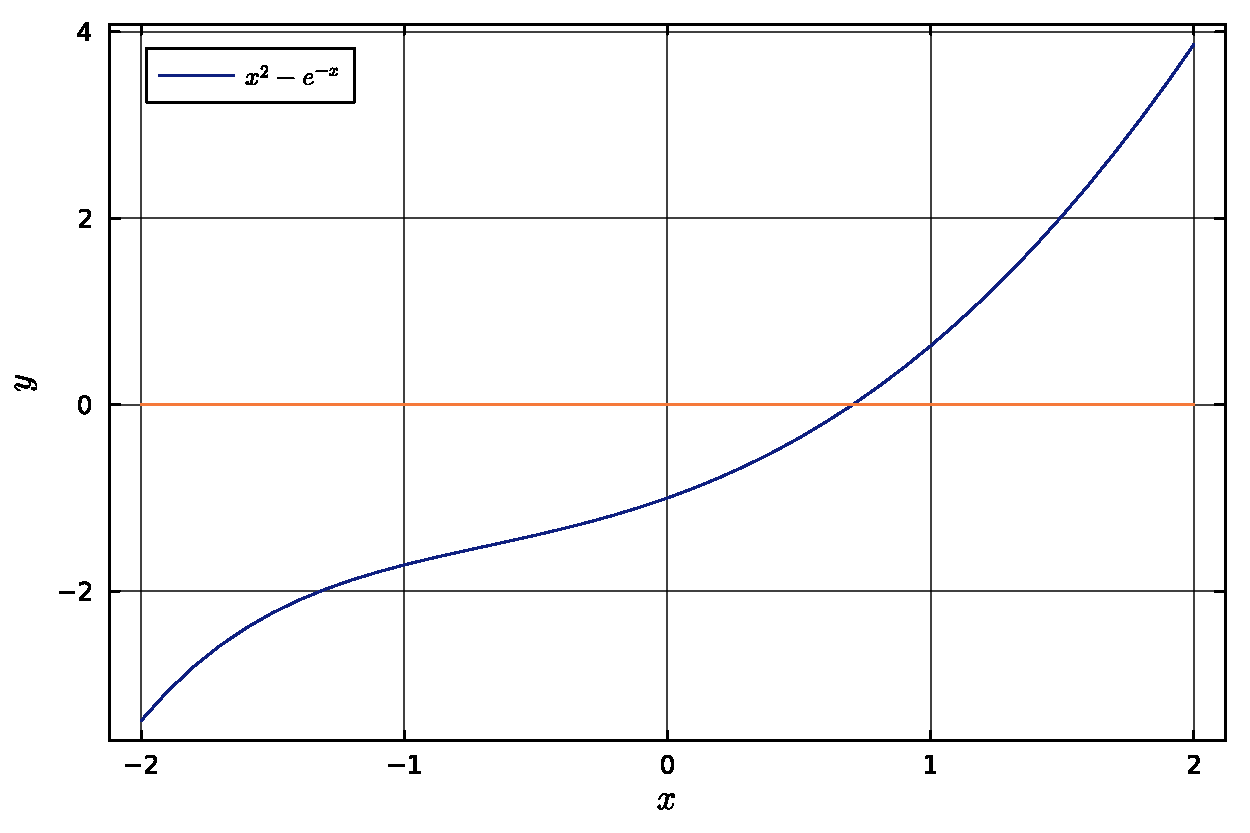
\includegraphics[width=\textwidth]{3321.pdf}
        \caption*{(a)}
    \end{minipage}
    \hspace{0.5cm}
    \begin{minipage}[b]{0.47\textwidth}
        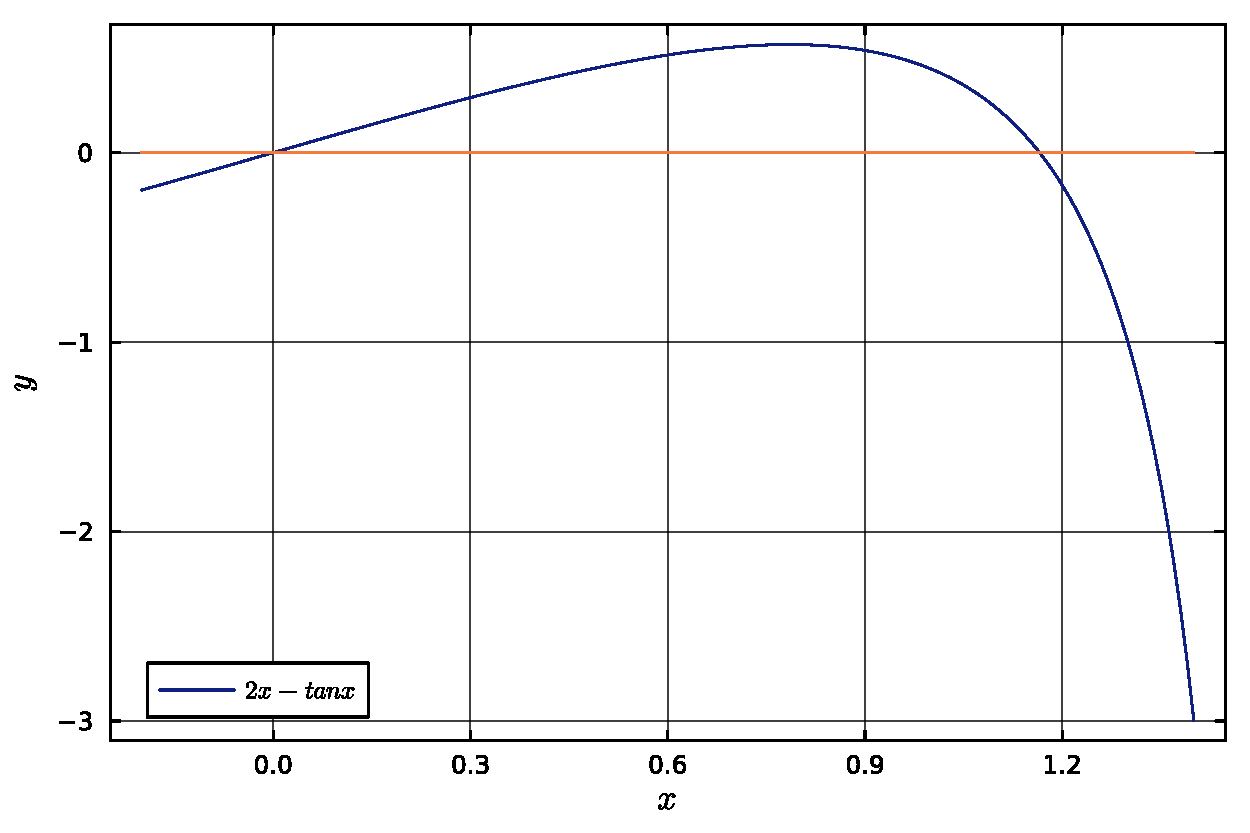
\includegraphics[width=\textwidth]{3322.pdf}
        \caption*{(b)}
    \end{minipage}

    \vspace{0.5cm}

    \begin{minipage}[b]{0.47\textwidth}
        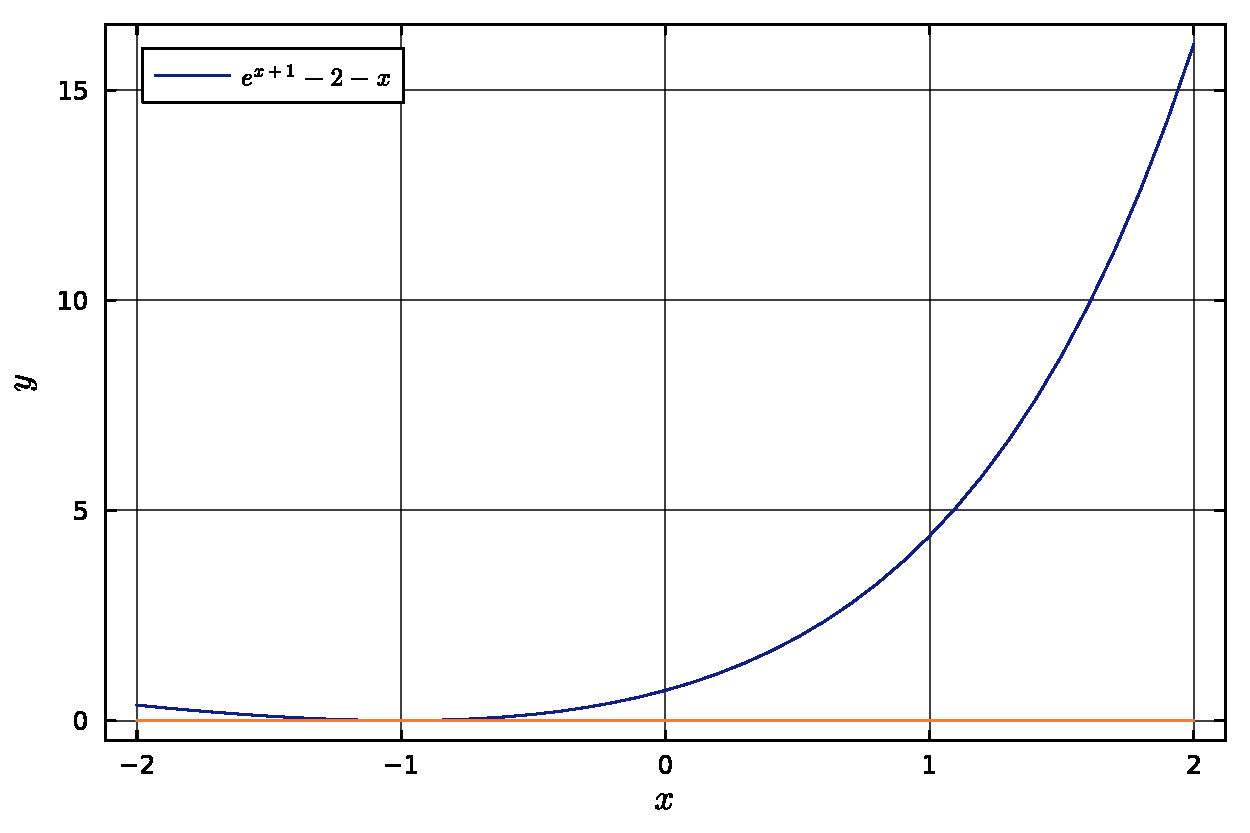
\includegraphics[width=\textwidth]{3323.pdf}
        \caption*{(c)}
    \end{minipage}
    \caption{Grafici delle funzioni $f_1$, $f_2$ e $f_3$.}
    \label{fig:es3_3_2_1}
\end{figure}

\paragraph{(2c) } L'algoritmo di Newton è stato applicato alle tre funzioni, con i seguenti risultati:
\begin{itemize}
    \item $f_1$: radice $x = 0.703$, in 8 iterazioni. Punto di partenza $x_0 = -2$.
    \item $f_2$: radici $x_1 = 0.000$, $x_2 = 1.166$, entrambe in 7 iterazioni. Punti di partenza $x_{0,1} = 0.65$, $x_{0,2} = 1.4$.
    \item $f_3$: radice $x = -1.000$ in 29 iterazioni. Punto di partenza $x_0 = 2$.
\end{itemize}

\paragraph{(2d) - Prima funzione}
Scopo dello studio dell'errore è verificare se i valori di $q$ e $C$ sono in accordo con quanto atteso.
In particolare ci aspettiamo che il metodo di Newton per questo particolare zero abbia $q = 2$ e 
$C = {\frac{1}{2}}\bigg|{\frac{f''(r)}{f'(r)}}\bigg| = 0.396$. Per determinare i valori di $q$, qui e nelle altre funzioni,
si fa riferimento alla formula \ref{eq:convergenza_bisezione_log}, e si calcola il rapporto tra i valori di 
$d_n$ e $d_{n+1}$; per determinare $C$, qui e nelle altre funzioni, si fa riferimento alla relazione 
$\lim_{n\to\infty} {\frac{|x_{n+1}-r|}{|x_n-r|^q}}= \lim_{n\to\infty} {\frac{|\epsilon_{n+1}|}{|\epsilon_n|^q}}=C$ \\
Si riportano i due grafici in figura \ref{fig:es3_3_2_2}.

\begin{figure}[!ht]
    \centering
    \begin{minipage}[b]{0.47\textwidth}
        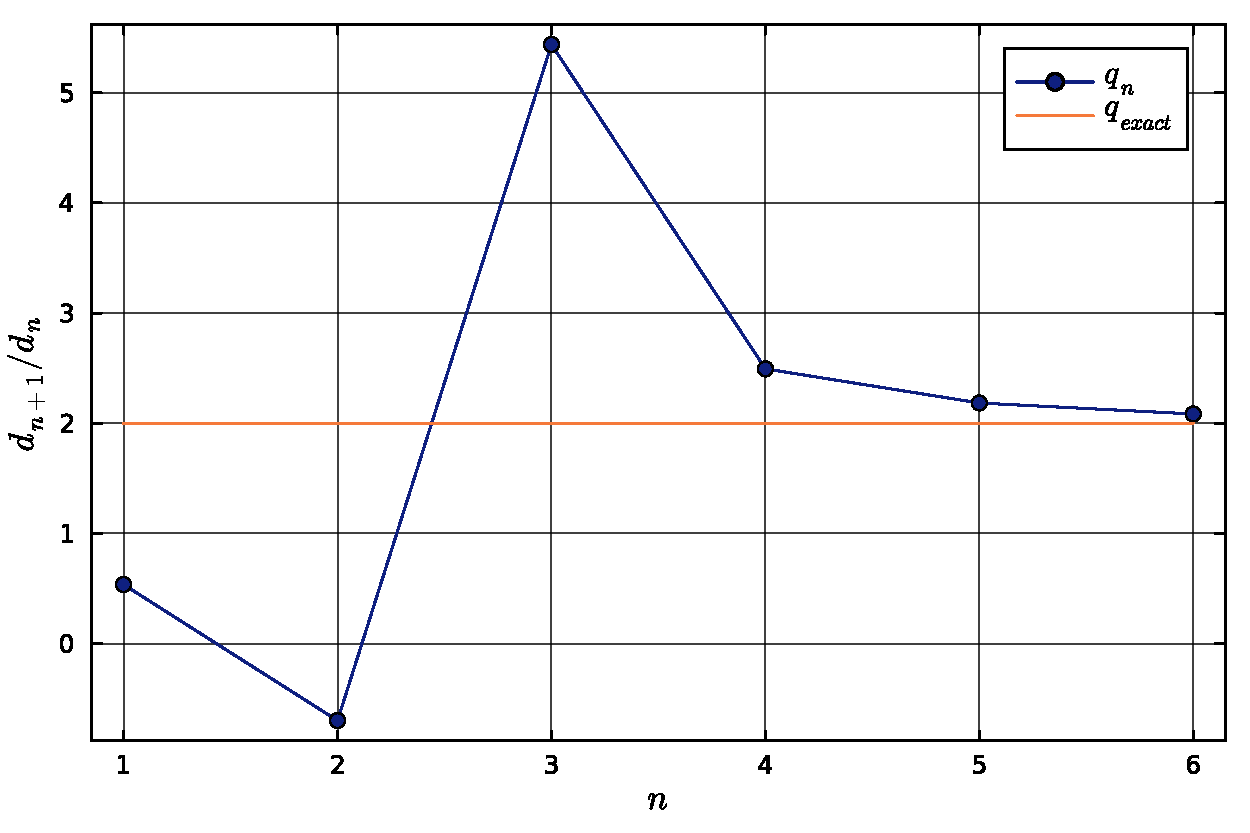
\includegraphics[width=\textwidth]{3321_q.pdf}
    \end{minipage}
    \hspace{0.5cm}
    \begin{minipage}[b]{0.47\textwidth}
        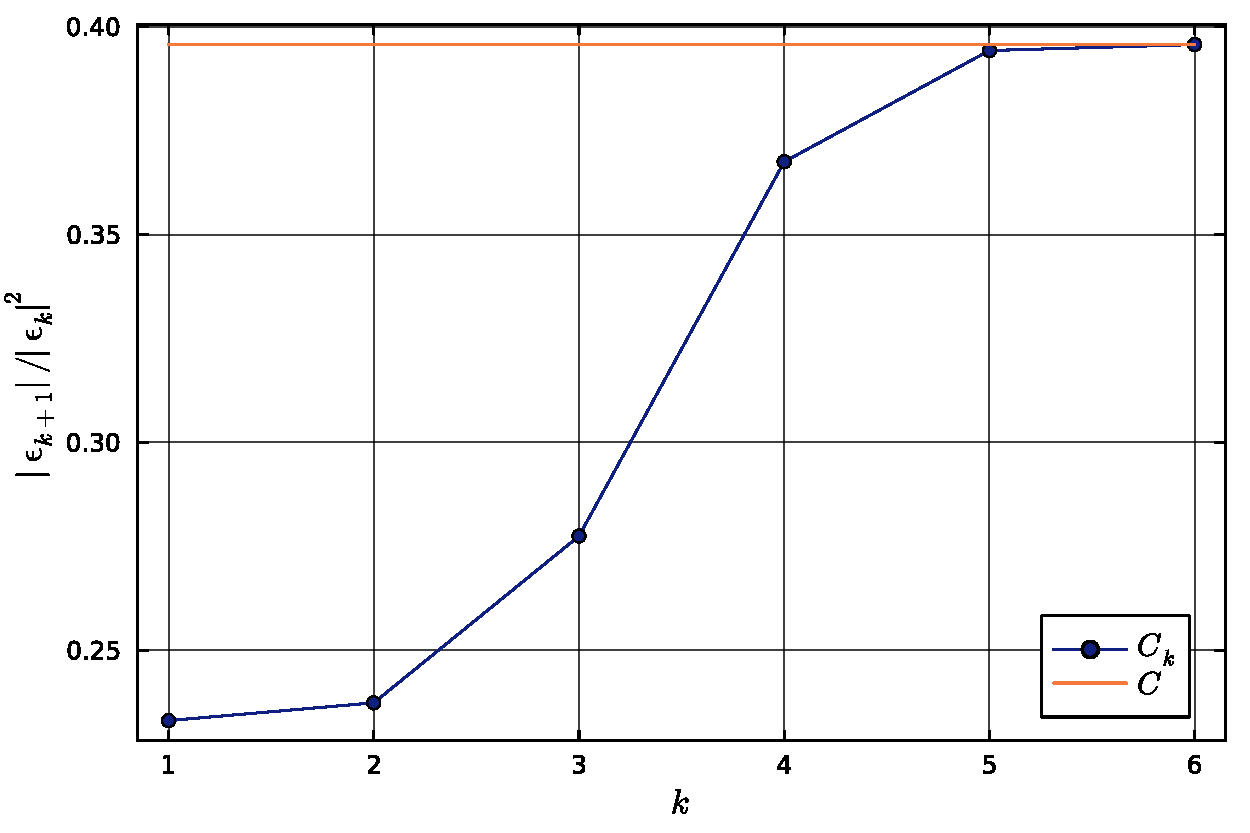
\includegraphics[width=\textwidth]{3321_C.pdf}
    \end{minipage}
    \caption{Studio del valore di $q$ e $C$ per $f_1$.}
    \label{fig:es3_3_2_2}
\end{figure}

Per le stime di $q$ e $C$ si è scelto di considerare l'ultimo punto della successione corrispondete, a causa
del numero limitato di iterazioni. Si ottiene:
\begin{equation}
    q = 2.084,
    \qquad
    C = 0.396.
\end{equation}
Si osserva che i valori ottenuti sono in accordo con quanto atteso, e quindi si può concludere che il metodo di
Newton converge in modo quadratico per la radice trovata.

\paragraph{(2d) - Seconda funzione}
\subparagraph{Prima radice, $x = 0.0$: }
È importante notare che la funzione $f_2$ in zero ha un andamento lineare, e perciò la sua derivata seconda è 
nulla. Questo implica che i valori di $q$ e $C$ non sono determinati dalle formule precedenti, perchè tali 
formule sono ricavate a partire da un'espansione di Taylor al secondo ordine. Per ovviare al problema 
si è scelto di ricavare le formule già utilizzate ma a ordine 3. I calcoli sono riportati nella cartella git
\verb|lab\computazionale1\esercizi\pen_and_paper.| \\
Di seguito sono riportati i valori per $q$ e $C$ con le dovute correzioni:
\begin{equation}
    q = 3,
    \qquad
    C = \frac{ f'''(r)}{3 f'(r)} = 0.667.
\end{equation}

In figura \ref{fig:es3_3_2_3} si riportano i grafici delle successioni $q_n$ e $C_n$ per la prima radice di $f_2$.

\begin{figure}[!ht]
    \centering
    \begin{minipage}[b]{0.47\textwidth}
        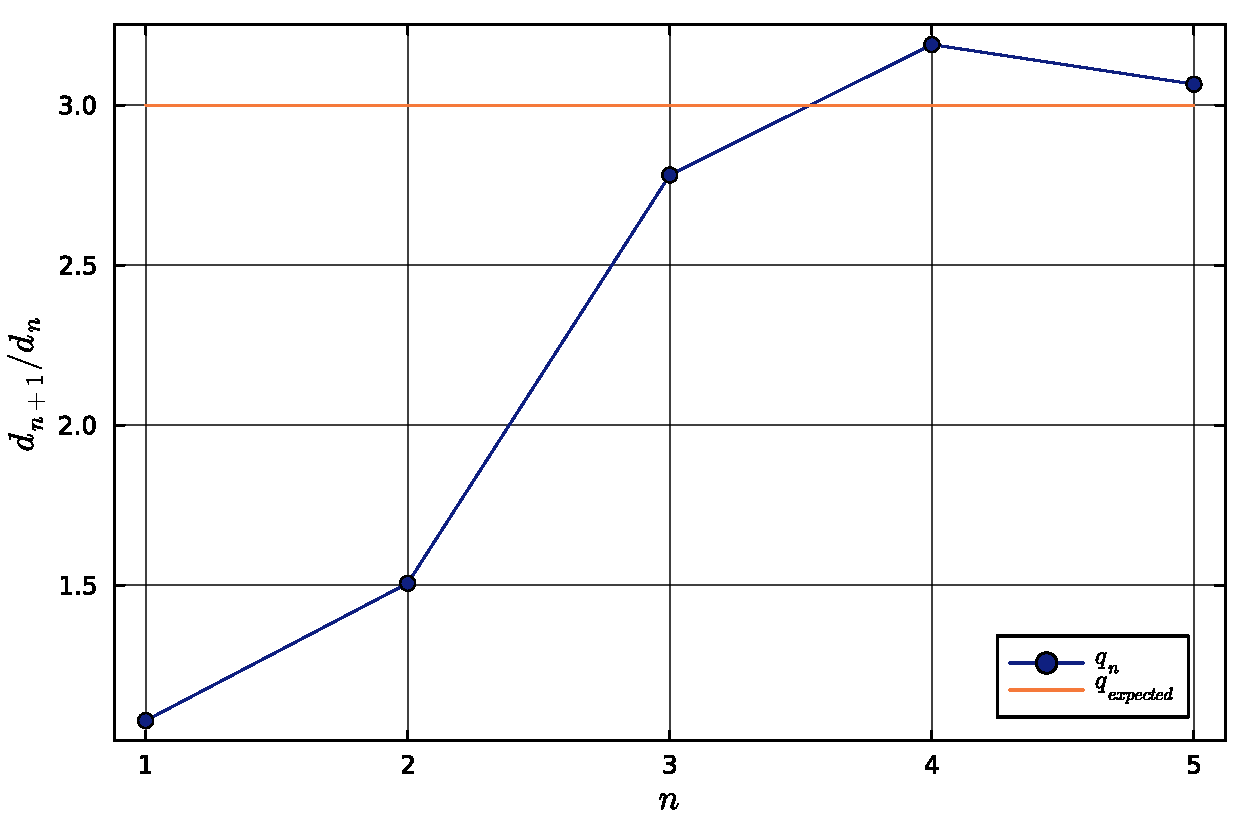
\includegraphics[width=\textwidth]{3322_q1.pdf}
    \end{minipage}
    \hspace{0.5cm}
    \begin{minipage}[b]{0.47\textwidth}
        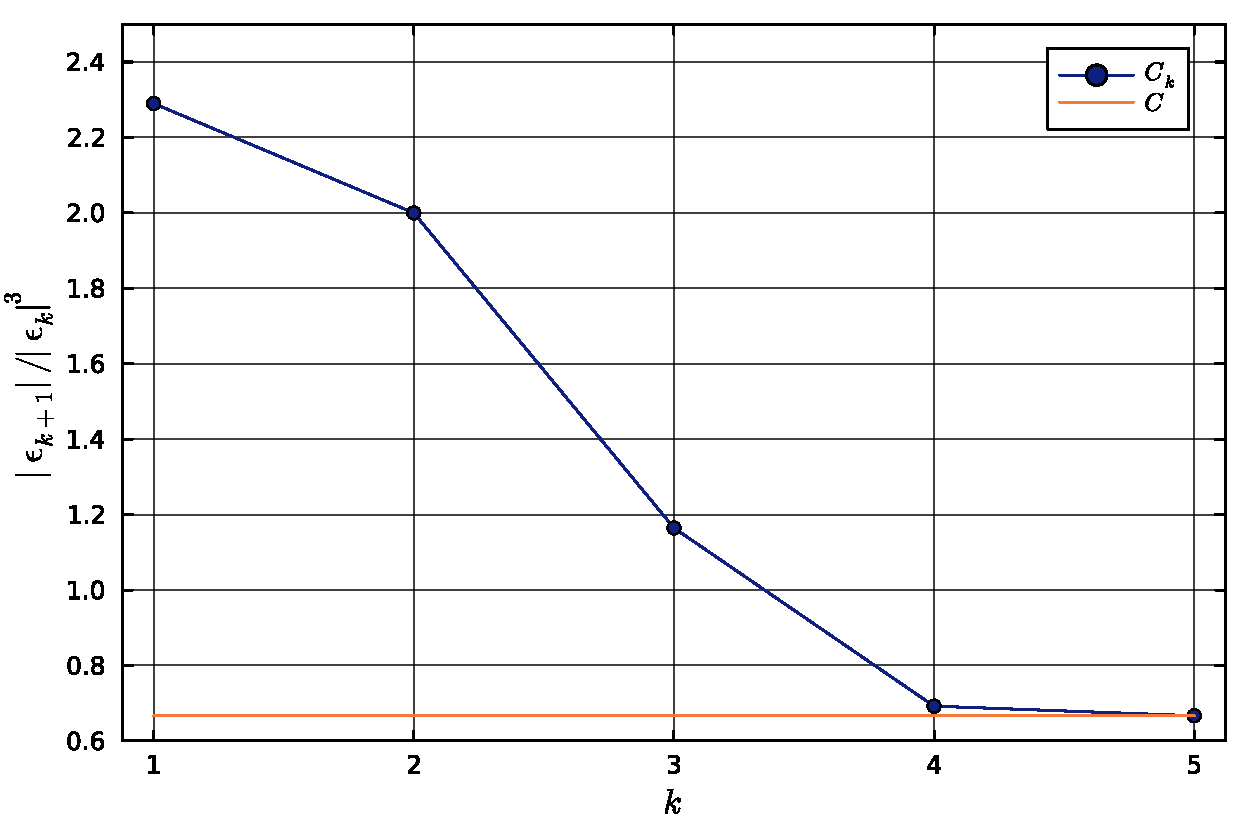
\includegraphics[width=\textwidth]{3322_C1.pdf}
    \end{minipage}
    \caption{Studio del valore di $q$ e $C$ per $f_2$., prima radice.}
    \label{fig:es3_3_2_3}
\end{figure}

Si ottengono i seguenti valori:
\begin{equation}
    q = 3.065,
    \qquad
    C = 0.667.
\end{equation}

Ci si può chiedere cosa succede se, non conoscendo l'andamento della funzione, si utilizzano le formule
precedenti. In particolare cosa succede se si fissa $q = 2$ e si stima $C$ come l'ultimo elemento della successione
$C_n = \frac{|x_{n+1}-r|}{|x_n-r|^2}$. L'aspettativa è che $C$ risulti nullo, dato che la derivata seconda
è nulla. Il grafico corrispondente può essere trovato nella cartella git
\verb|lab_computazionale1\esercizi\3_3_2.ipynb|, e mostra che il valore di $C$ è effettivamente nullo. \\ 

\subparagraph{Seconda radice, $x = 1.166$: } la seconda radice di $f_2$ non presenta problemi, così le formule
sono quelle viste inizialmente. I valori attesi sono $q = 2$ e $C = 3.383$. 
Si riportano i grafici delle successioni $q_n$ e $C_n$ in figura \ref{fig:es3_3_2_4}.
\begin{figure}[!ht]
    \centering
    \begin{minipage}[b]{0.47\textwidth}
        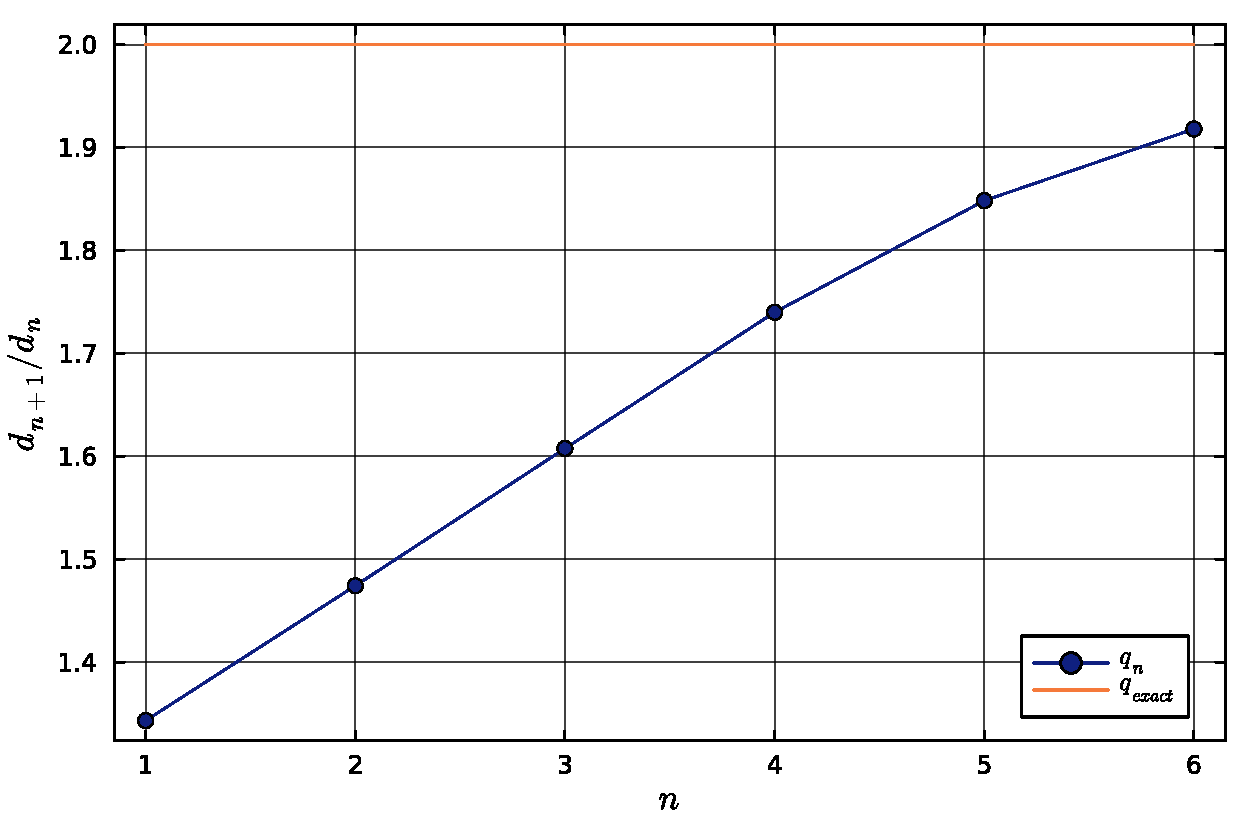
\includegraphics[width=\textwidth]{3322_q2.pdf}
    \end{minipage}
    \hspace{0.5cm}
    \begin{minipage}[b]{0.47\textwidth}
        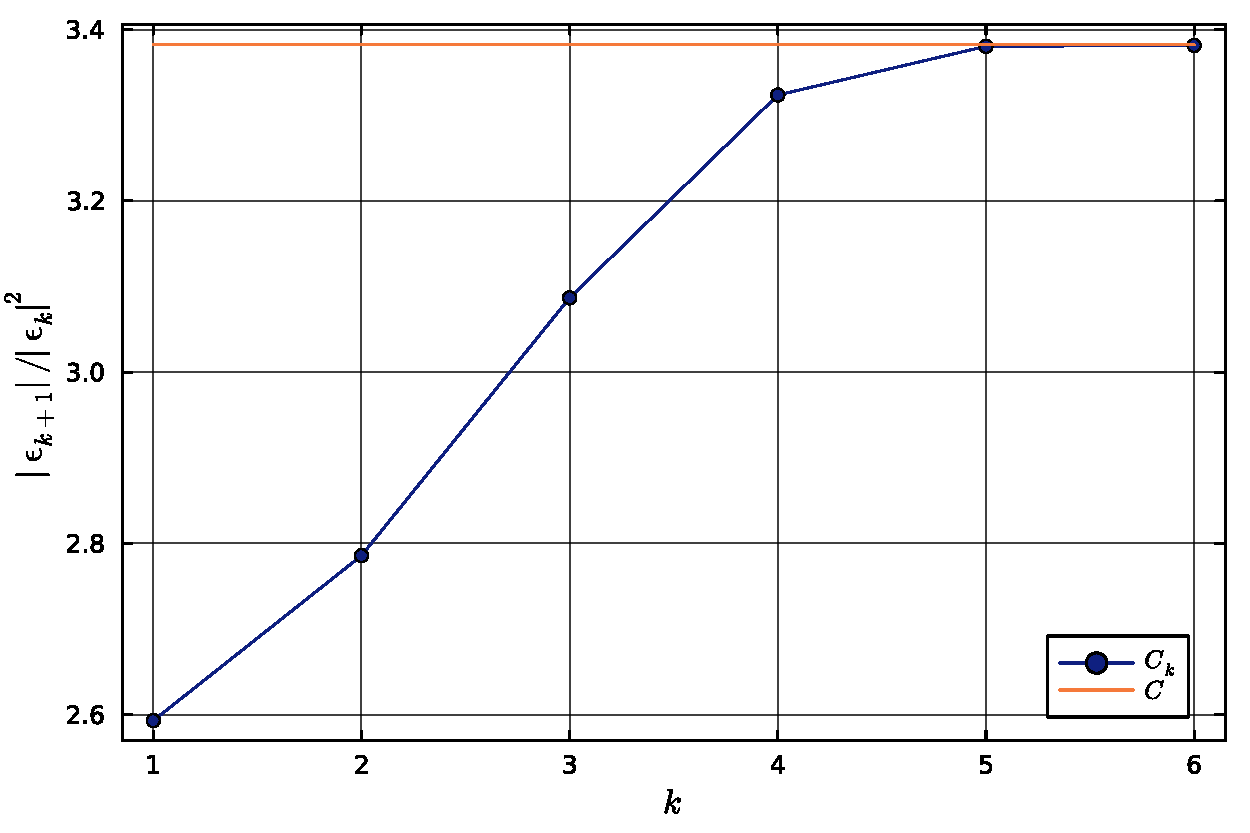
\includegraphics[width=\textwidth]{3322_C2.pdf}
    \end{minipage}
    \caption{Studio del valore di $q$ e $C$ per $f_2$, seconda radice.}
    \label{fig:es3_3_2_4}
\end{figure}
Si ottengono i seguenti valori:
\begin{equation}
    q = 2.000,
    \qquad
    C = \frac{ f''(r)}{2 f'(r)} = 3.382.
\end{equation}
In accordo con quanto atteso, il metodo di Newton converge in modo quadratico per la radice trovata.

\paragraph{(2d) - Terza funzione}
Osservando il grafico della funzione $f_3$ si nota che la radice è un punto di minimo, e quindi ha una molteplicità
$m$. D'altra parte, possiamo intuire che la radice di $f_3$ ha una molteplicità anche dal numero di iterazioni,
molto elevato rispetto alle altre funzioni. \\
Come è noto dalla teoria, il metodo di Newton in caso di radici multiple converge linearmente, e nella formula
$ \epsilon_{n+1} = C (\epsilon_n)^q $ ci aspettiamo $q = 1$. Inoltre in caso di radici multiple
la costante d'errore asintotica diviene $(1-{\frac{1}{m}})$. \\

Il primo passo è verificare il valore di $q$. Si riporta in figura \ref{fig:es3_3_2_6} il grafico 
della successione $q_n$, da cui possiamo confermare stimare $q = 1.067$. \\

Si riportano in figura \ref{fig:es3_3_2_6} i grafici della successione $C_n$, una volta senza considerare 
la molteplicità della radice, e una volta considerando la molteplicità della radice.
\begin{figure}[!ht]
    \centering
    \begin{minipage}[b]{0.6\textwidth}
        \centering
        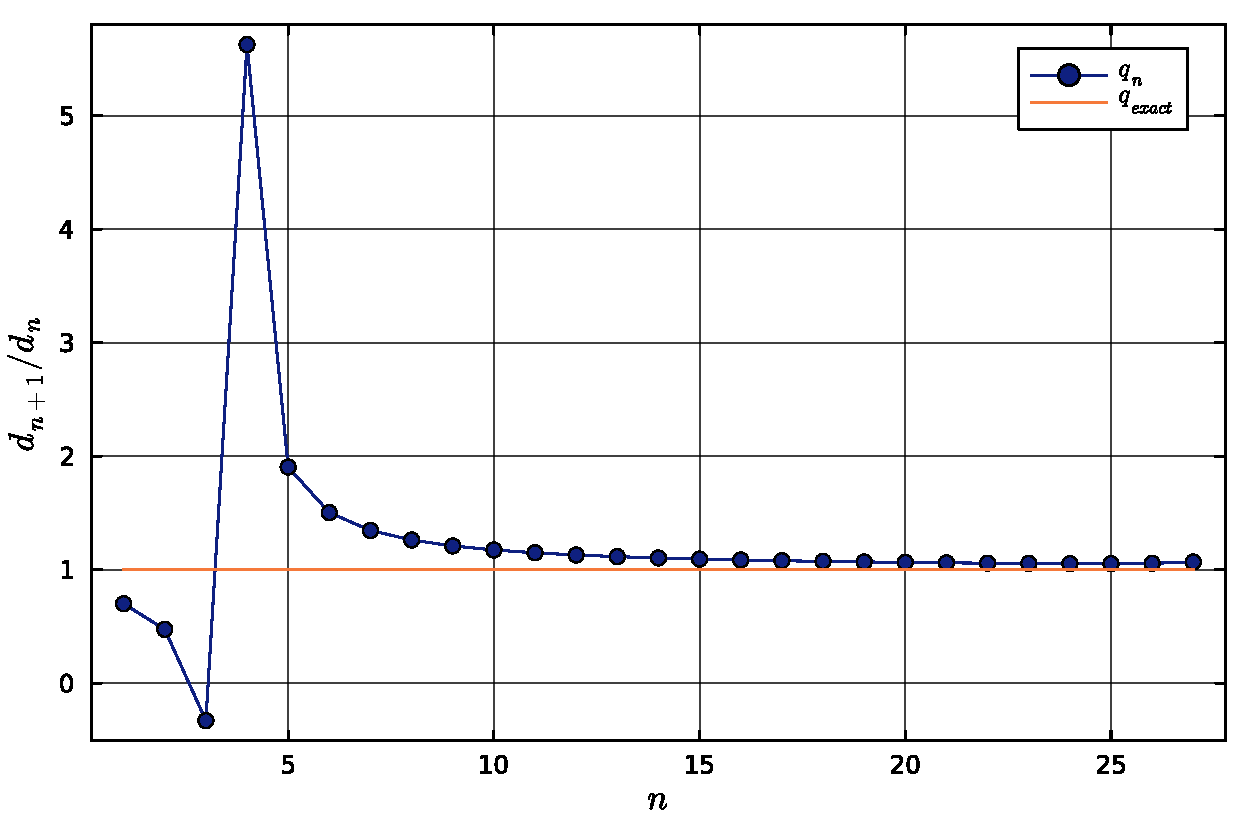
\includegraphics[width=0.8\textwidth]{3323_q.pdf}
        \caption*{}
    \end{minipage}
    \vspace{0.5cm}

    \begin{minipage}[b]{0.47\textwidth}
        \centering
        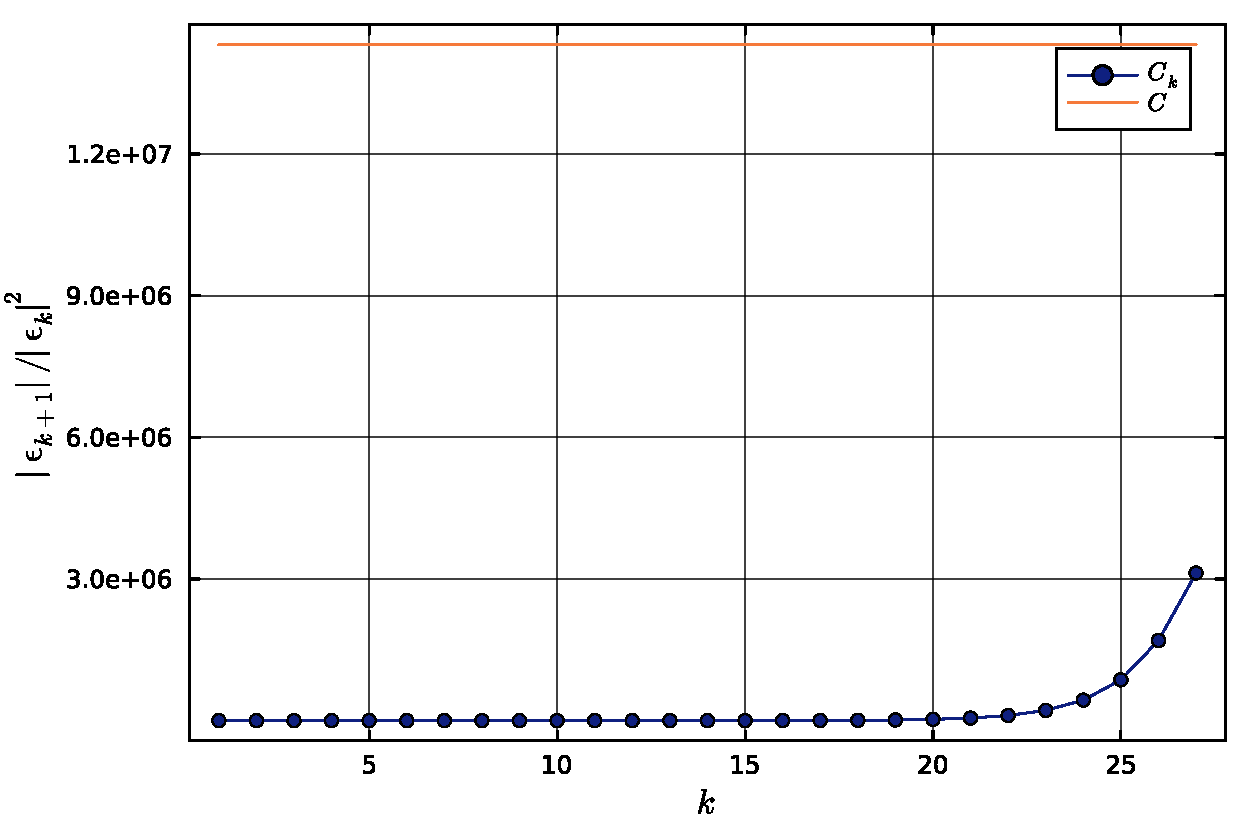
\includegraphics[width=\textwidth]{3323_C1.pdf}
        \caption*{}
    \end{minipage}
    \hspace{0.5cm}
    \begin{minipage}[b]{0.47\textwidth}
        \centering
        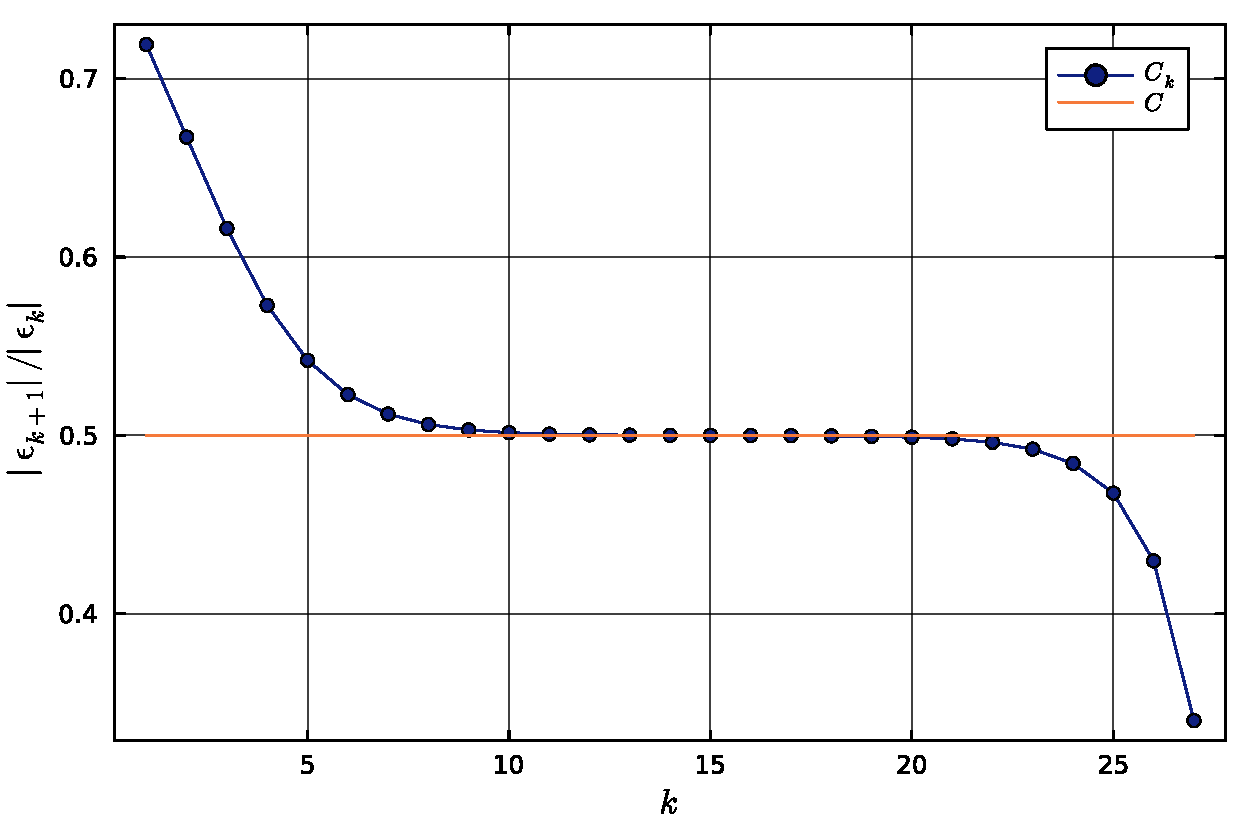
\includegraphics[width=\textwidth]{3323_C2.pdf}
        \caption*{}
    \end{minipage}

    \caption{Studio del valore di $q$ (sopra) e $C$ (sotto) per $f_3$.}
    \label{fig:es3_3_2_6}
\end{figure}

Come si può notare da \ref{fig:es3_3_2_6}, non avendo considerato la molteplictà della radice, il valore di $C$
si discosta molto da quello calcolato con la solita formula $C = \frac{ f''(r)}{2 f'(r)}$. Invece, nel secondo 
grafico della stessa figura si osserva che i valori successivi di $C_n$ si stabilizzano attorno al valore 
$C = 0.5$, per poi calare nuovamente a causa di errori di cancellazione numerica. \\
Scegliendo $C = C_{15}$ come stima del plateau si ottengono i seguenti valori:
\begin{equation}
    C = 0.500,
    \qquad
    m = 2.000,
    \qquad
\end{equation}
in accordo con quanto atteso. 

\subsection{Esercizio 3.3.3}
\label{sec:333}
Traccia la funzione $f(x)=x^{-2} - \sin x$ nell'intervallo $x \in [0.5,10]$.  
Per ciascun valore iniziale $x_1=1,\, x_1=2,\,\ldots,\, x_1=7$, applica il metodo di Newton a $f$  
e realizza una tabella che mostri $x_1$ e la radice trovata dal metodo.  
In quale caso l'iterazione converge a una radice diversa da quella più vicina al valore iniziale?  
Usa il grafico per spiegare perché ciò è accaduto.

\subsubsection{Soluzione}
Si riporta in figura \ref{fig:es3_3_3_1} il grafico della funzione $f(x)=x^{-2} - \sin x$ nell'intervallo
$[0.5,10]$, con i punti di partenza del metodo di Newton. 
\begin{figure}[!ht]
    \centering
    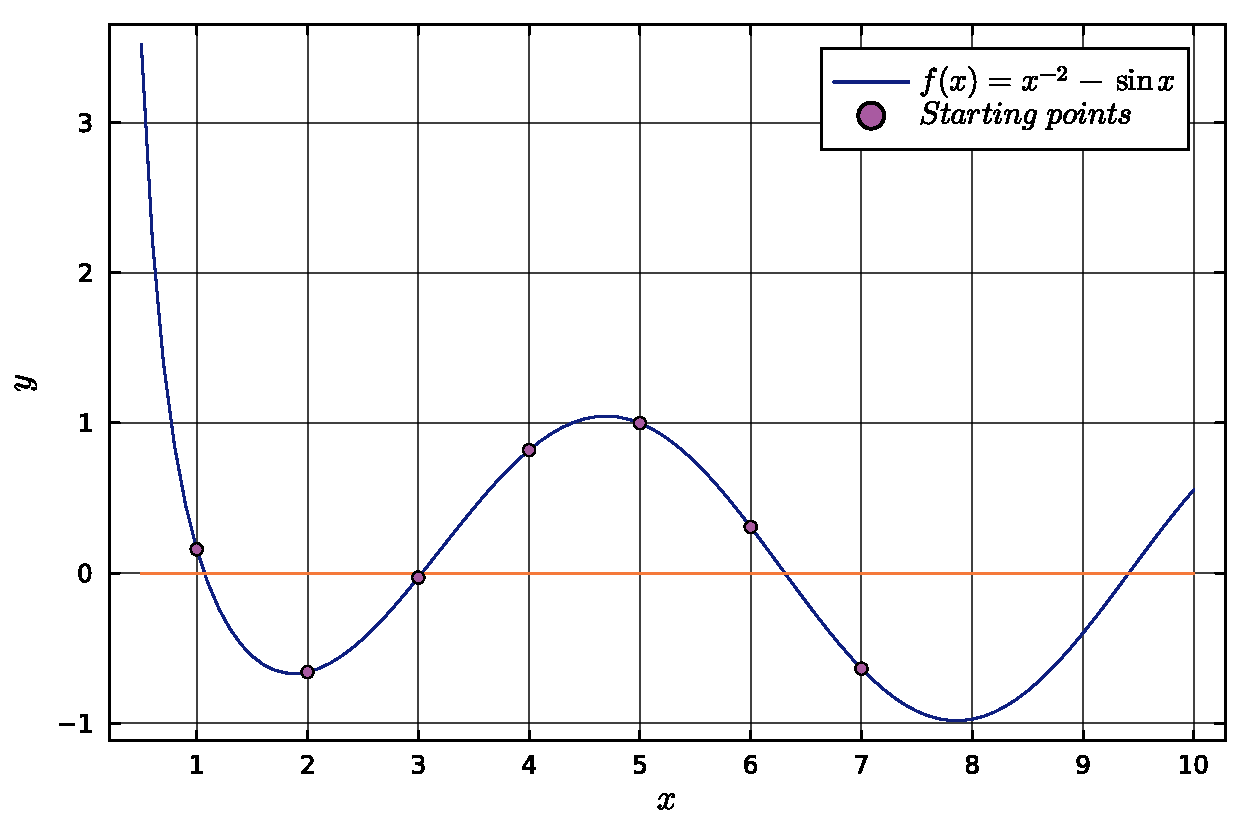
\includegraphics[width=0.8\textwidth]{3331.pdf}
    \caption{Grafico della funzione $f(x)=x^{-2} - \sin x$ nell'intervallo $[0.5,10]$.}
    \label{fig:es3_3_3_1}
\end{figure}

Applicando il metodo di Newton con i valori iniziali, non sempre si ottengono le radici più vicine al valore
di partenza. Si riportano i risultati in tabella \ref{tab:es3_3_3_1}.

\begin{table}[!ht]
\centering
\caption{Valori relativi ai punti \( x_1, \dots, x_7 \)}
\label{tab:es3_3_3_1}
\begin{tabularx}{\textwidth}{|l!{\vrule width 2pt}*{7}{>{\centering\arraybackslash}X|}}
\hline
 & \( x_1 = 1 \) & \cellcolor{orange}\( x_2 = 2 \) & \( x_3 = 3 \) & \( x_4 = 4 \) & \cellcolor{orange}\( x_5 = 5 \) & \( x_6 = 6 \) & \( x_7 = 7 \) \\
\specialrule{.1em}{0em}{0em}  % linea più spessa
\( x_{\text{start}} \) & 1.0 & \cellcolor{orange}2.0 & 3.0 & 4.0 & \cellcolor{orange}5.0 & 6.0 & 7.0 \\
\hline
\( x_{\text{root}} \)  & 1.1 & \cellcolor{orange}6.3 & 3.0 & 3.0 & \cellcolor{orange}9.4 & 6.3 & 6.3 \\
\hline
\( f'(x) \)            & -2.5 & \cellcolor{orange}0.2 & 0.9 & 0.6 & \cellcolor{orange}-0.3 & -0.9 & -0.8 \\
\hline
\end{tabularx}
\end{table}

Le due colonne evidenziate in arancione sono i punti iniziali che non convergono alla radice più vicina. 
Osservando il grafico della funzione è facile osservare che i punti iniziali $x_2$ e $x_5$ sono vicini a
un minimo e a un massimo locali, rispettivamente. In effetti la derivata prima in questi punti è vicina a zero,
come riportato in tabella. Non è esattamente zero, altrimenti il caso sarebbe quello della seconda funzione 
all'esercizio 3.3.2, ma è comunque piccola: ciò significa che il metodo di Newton converge quadraticamente, ma
non necessariamente alla radice più vicina. \\

\subsection{Esercizio 3.3.4}
Le proprietà più facilmente osservabili dell'orbita di un corpo celeste attorno al Sole sono il periodo $\tau$ 
e l'eccentricità ellittica $\epsilon$. (Un cerchio ha $\epsilon=0$.) Da questi parametri è possibile determinare, 
in ogni istante $t$, la \textit{vera anomalia} $\theta(t)$. Questa è l'angolo tra la direzione del perielio 
(il punto dell'orbita più vicino al Sole) e la posizione attuale del corpo, visto dal fuoco principale 
dell'ellisse (dove si trova il Sole). Questo si ottiene tramite

\begin{equation}
    \label{eq:eq-kepler1}
    \tan \frac{\theta}{2} = \sqrt{\frac{1+\epsilon}{1-\epsilon}}\,
    \tan \frac{\psi}{2}\,
\end{equation}
dove l'\textit{anomalia eccentrica} $\psi(t)$ soddisfa l'equazione di Keplero:
\begin{equation}
    \label{eq:eq-kepler2}
    \psi - \epsilon \sin \psi - \frac{2\pi t}{\tau} = 0\,.
\end{equation}
L'equazione \ref{eq:eq-kepler2} deve essere risolta numericamente per trovare $\psi(t)$, 
e poi la \ref{eq:eq-kepler1} può essere risolta analiticamente per ottenere $\theta(t)$.
L'asteroide Eros ha $\tau=1.7610$ anni e $\epsilon=0.2230$. Utilizzando il metodo di Newton per la \ref{eq:eq-kepler2}, 
realizza un grafico di $\theta(t)$ per 100 valori di $t$ compresi tra $0$ e $\tau$, cioè per un'orbita completa.\\
(Nota: usa $\verb|mod|(\theta,2\pi)$ per riportare l'angolo tra 0 e $2\pi$ se vuoi che il risultato 
sia una funzione continua.)

\subsection{Soluzione}
Per prima cosa si è risolta l'equazione \ref{eq:eq-kepler2} con il metodo di Newton. Per capire meglio il 
procedimento si riporta l'equazione \ref{eq:eq-kepler2} nel grafico sinistro di \ref{fig:es3_3_4_1}, 
dove si osserva che 
la funzione ha un solo zero nell'intervallo $[0,2\pi]$. Il metodo di Newton è stato applicato al variare
del tempo $t$, cioè è stato applicato alla stessa funzione ma traslata in verticale, come si può vedere
nella figura. \\
\begin{figure}[!ht]
    \centering
    \begin{minipage}[b]{0.47\textwidth}
        \centering
        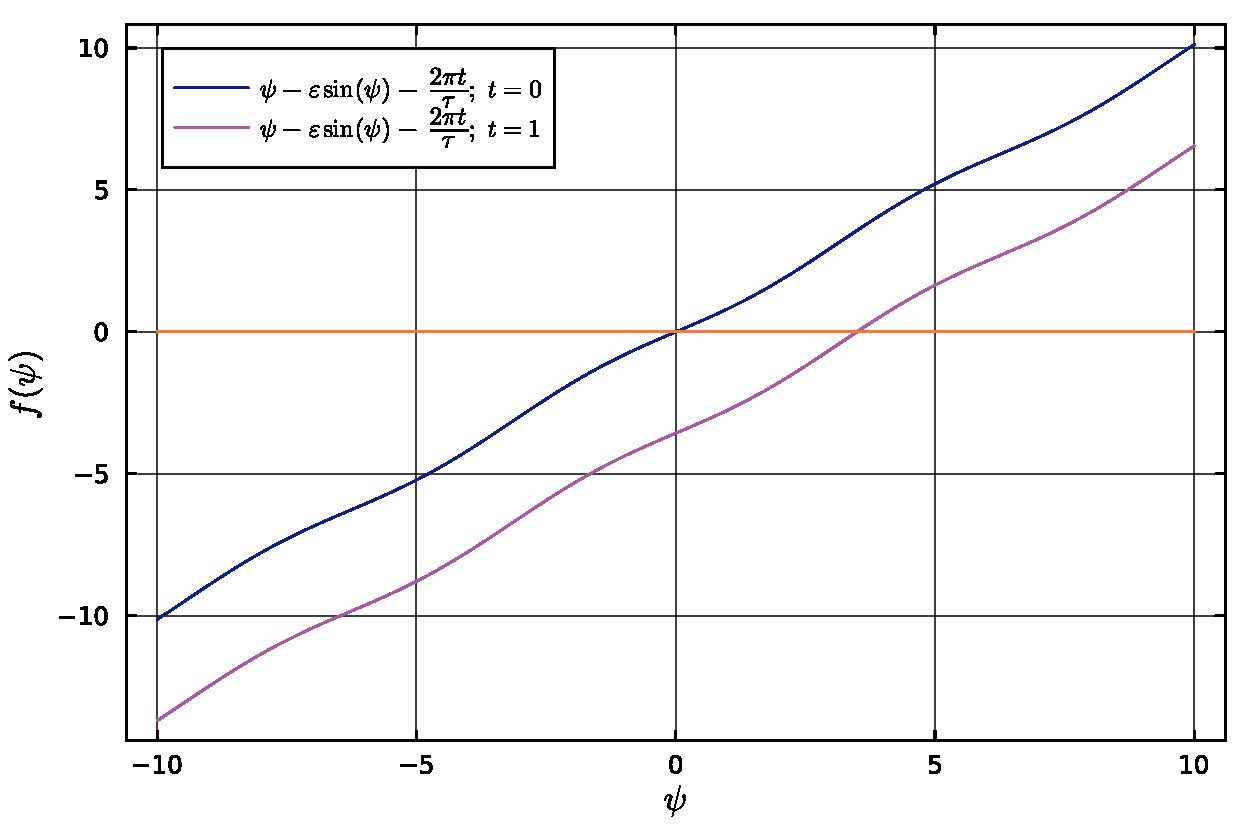
\includegraphics[width=\textwidth]{3341.pdf}
        \caption*{}
    \end{minipage}
    \hspace{0.5cm}
    \begin{minipage}[b]{0.47\textwidth}
        \centering
        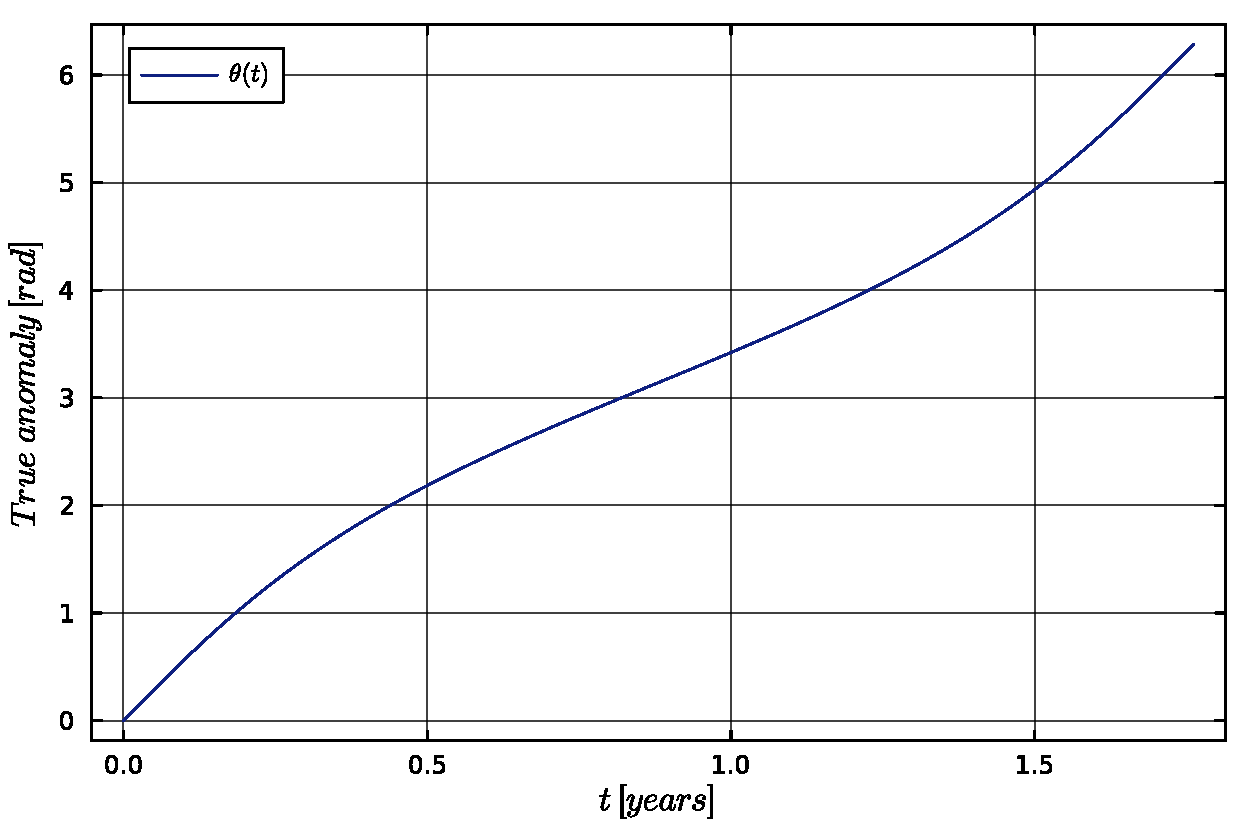
\includegraphics[width=\textwidth]{3342.pdf}
        \caption*{}
    \end{minipage}
    \caption{Grafico dell'equazione \ref{eq:eq-kepler2} (sinistra) e $\theta(t)$ (destra).}
    \label{fig:es3_3_4_1}    
\end{figure}
\\
Ottenuti i valori di $\psi$ in corrispondenza dei 100 valori di $t$ compresi tra $0$ e $\tau$, si è calcolata
la vera anomalia $\theta$ tramite la relazione \ref{eq:eq-kepler1}. Si riporta il grafico di $\theta(t)$ in
figura sinistra di \ref{fig:es3_3_4_1}.

\subsection{Esercizi 3.4.1, 3.4.2}
1. Scrivi un programma che implementi il metodo della secante. \\
2. Per ciascuna delle seguenti funzioni, esegui i seguenti passi. \\
(a) Riscrivi l'equazione nella forma standard per la ricerca degli zeri, $f(x) = 0$. \\
(b) Traccia il grafico di $f$ nell'intervallo indicato e determina quante radici sono presenti nell'intervallo. \\
(c) Per ciascuna radice determina un intervallo che la racchiuda. Poi usa il metodo della secante, 
    partendo dagli estremi dell'intervallo, per trovare ciascuna radice.\\
(d) Per una delle radici, usa gli errori nella sequenza della secante per determinare numericamente 
    se la convergenza è apparentemente compresa tra lineare e quadratica.\\
1. $x^2=e^{-x}$, su $[-2,2]$ \\
2. $2x = \tan x$, su $[-0.2,1.4]$ \\
3. $e^{x+1}=2+x$, su $[-2,2]$ \\

\subsubsection{Soluzione}
\paragraph{(1) } Si è implementato il metodo della secante e lo si è testato con la funzione $x^2 - 1$, 
ottenedo come radice $x = 1.0$ in 10 iterazioni. 

\paragraph{(2a)-(2b) } Per questi esercizi si rimanda alle sezioni \ref{sec:332_2a} e \ref{sec:332_2b}.

\paragraph{{(2c) } } L'algoritmo della secante è stato applicato alle tre funzioni, con i seguenti risultati:
\begin{itemize}
    \item $f_1$: radice $x = 0.703$, in 9 iterazioni. Intervallo iniziale $[1,2]$.
    \item $f_2$: radici $x_1 = 0.000$, $x_2 = 1.166$, in 6 e 11 iterazioni, rispettivamente. Intervalli iniziali:
    $[-0.1,0.2]$ e $[0.9,1.3]$.
    \item $f_3$: radice $x = -1.000$ in 42 iterazioni. Intervallo iniziale $[-2,0]$.
\end{itemize}

In generale si può notare che il numero di iterazioni nel metodo della secante è maggiore rispetto 
a quello del metodo di Newton, nonostante gli intervalli iniziali nel caso della secante siano stati scelti 
in modo da essere molto vicini alla radice. Ciò è dovuto al fatto che il metodo della secante converge
con ordine del rapporto aureo, mentre il metodo di Newton converge con ordine quadratico per radici semplici. \\

\paragraph{(2d) } Si è scelto di studiare l'errore della secante per la radice di $f_1$. Si riporta in figura
\ref{fig:es3_4_2_1} il grafico della successione $d_k = |x_k - x_{k-1}|$. Come stima di $q$ si è scelto di
considerare l'ultimo punto della successione, e si ottiene $q = 1.692$, sufficientemente in accordo con 
$q_{atteso} = 1.618$.
\begin{figure}[!ht]
    \centering
    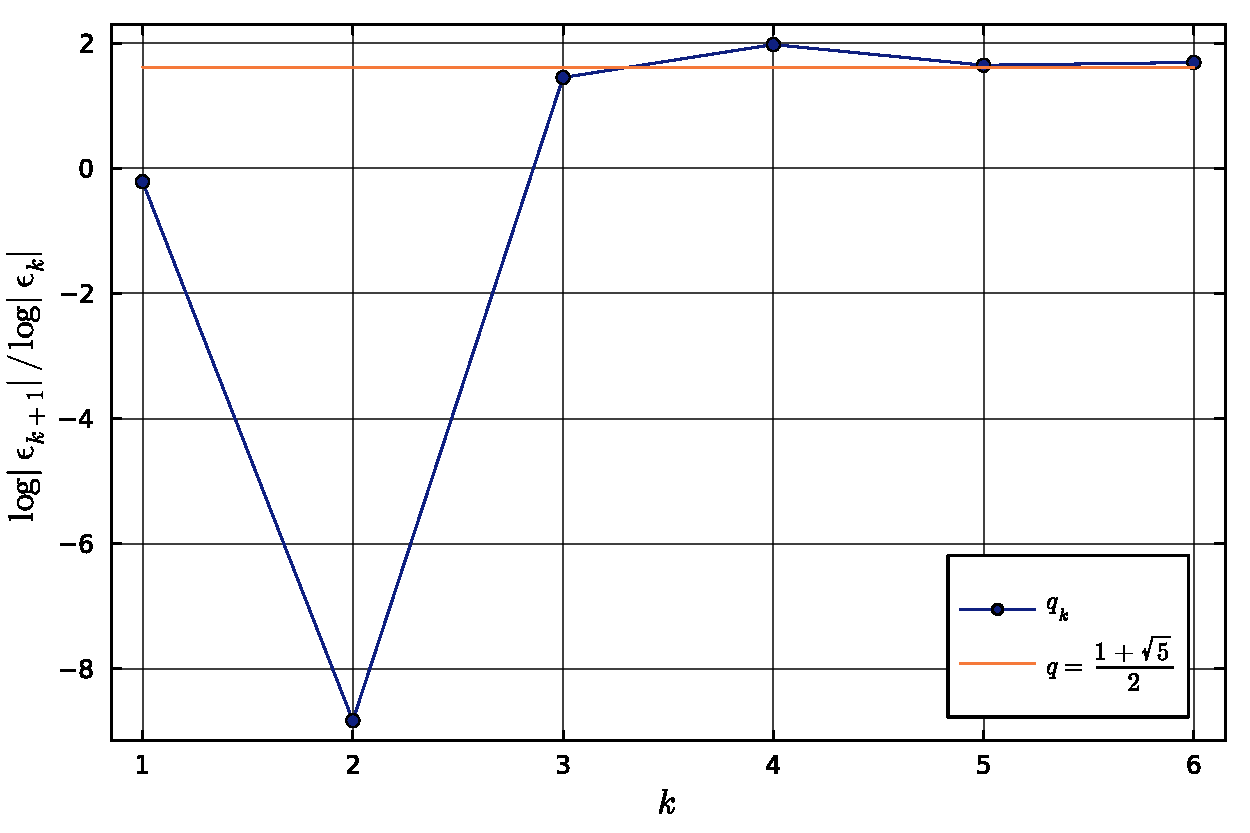
\includegraphics[width=0.8\textwidth]{3421.pdf}
    \caption{Studio del valore di $q$ per la radice di $f_1$.}
    \label{fig:es3_4_2_1}
\end{figure}

\subsection{Esercizio 3.4.3}
Utilizza un grafico per localizzare approssimativamente tutte le radici di $f(x)=x^{-2}-\sin(x)$ 
nell'intervallo $[0.5,10]$. 
Poi trova una coppia di punti iniziali per ciascuna radice tale che il metodo della secante converga 
a quella radice.

\subsubsection{Soluzione}
Si riporta in figura \ref{fig:es3_4_3_1} il grafico della funzione $f(x)=x^{-2}-\sin(x)$ nell'intervallo
$[0.5,10]$, da cui si evince che la funzione ha 4 radici nell'intervallo. In figura sono riportate anche
le radici stimate.
\begin{figure}[!ht]
    \centering
    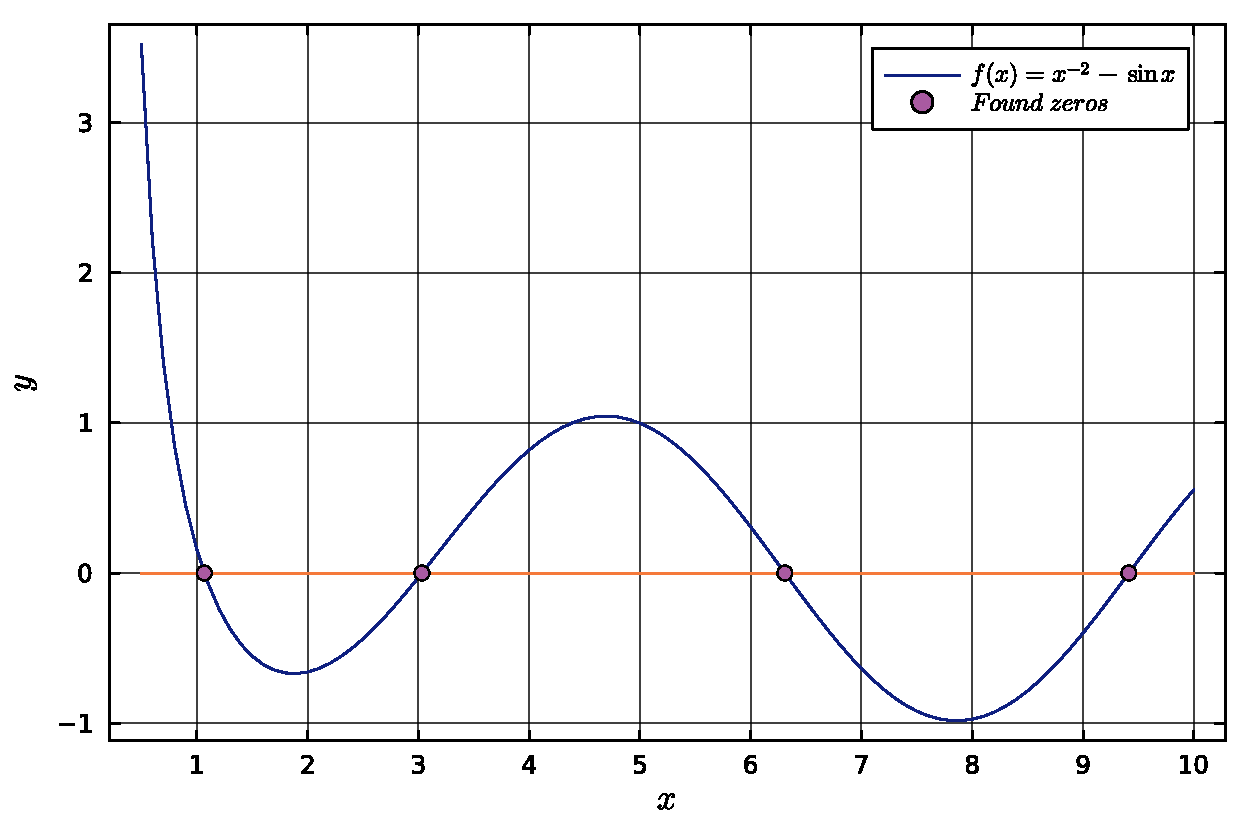
\includegraphics[width=0.8\textwidth]{3431.pdf}
    \caption{Grafico della funzione $f(x)=x^{-2}-\sin(x)$ nell'intervallo $[0.5,10]$.}
    \label{fig:es3_4_3_1}
\end{figure}

Si riportano in tabella \ref{tab:es3_4_3_1} le radici stimate, i punti iniziali scelti e il numero di iterazioni
necessarie per la convergenza.
\begin{table}[!ht]
    \centering
    \begin{tabular}{|c|c|c|c|}
        \hline
        \textbf{Radice} & \textbf{Radice stimata} & \textbf{Punti iniziali} & \textbf{Numero di iterazioni} \\
        \hline
        $r_1$ & $1.068$  & $[1.0,\,2.0]$   & 11  \\
        $r_2$ & $3.033$  & $[2.0,\,4.0]$   & 8  \\
        $r_3$ & $6.308$  & $[6.0,\,7.0]$   & 7  \\
        $r_4$ & $9.413$  & $[9.0,\,10.0]$  & 7  \\
        \hline
    \end{tabular}
    \caption{Radici stimate e punti iniziali per il metodo della secante.}
    \label{tab:es3_4_3_1}
\end{table}
Possiamo osservare che le radici trovate sono in accordo con quelle stimate nell'esercizio \ref{sec:333} 
con metodo di Newton.

\section{Interpolazioni}
%Se hai tempo inserisci l'esercizio 4.1.1, matrice di Vandermonde.

\subsection{Esercizi 4.2.1, 4.2.2}
1. Scrivi un programma che implementi la formula baricentrica dell'interpolazione di Lagrange 
    per nodi in posizioni generiche. \\
2. In ciascun caso, interpola la funzione data usando $n$ nodi equispaziati nell'intervallo indicato.
    Rappresenta graficamente ciascuna funzione interpolante insieme alla funzione esatta. \\
(a) $f(x) = \ln (x), \quad n = 2,3,4, \quad x\in [1,10]$ \\ 
(b) $f(x) = \tanh (x), \quad n = 2,3,4, \quad x \in [-3,2]$ \\
(c) $f(x) = \cosh (x), \quad n = 2,3,4, \quad x \in [-1,3]$ \\
(d) $f(x) = |x|, \quad n = 3,5,7, \quad x \in [-2,1]$ \\

\subsubsection{Soluzione}
\paragraph{(1) } Si è implementata la formula baricentrica dell'interpolazione di Lagrange 
per nodi in posizioni generiche, e la si è testata nell'esercizio 4.2.2.
\paragraph{(2) } In questo esercizio, nonostante sia data la possibilità di utilizzare la formula baricentrica
semplificata dai nodi equispaziati, si è scelto di utilizzare la formula baricentrica per nodi generici, come
test dell'implementazione dell'esercizio precedente. In esercizi successivi sarà richiesto di implementare
la formula baricentrica per nodi di Chebyshev, e in tale contesto si è sviluppata una funzione Julia che
chiede la natura dei nodi e restituisce la funzione baricentrica corrispondente, anche per il caso equispaziato. \\
Si riportano i grafici delle funzioni interpolanti in figura \ref{fig:es4_2_2_1}.
\begin{figure}[!ht]
    \centering
    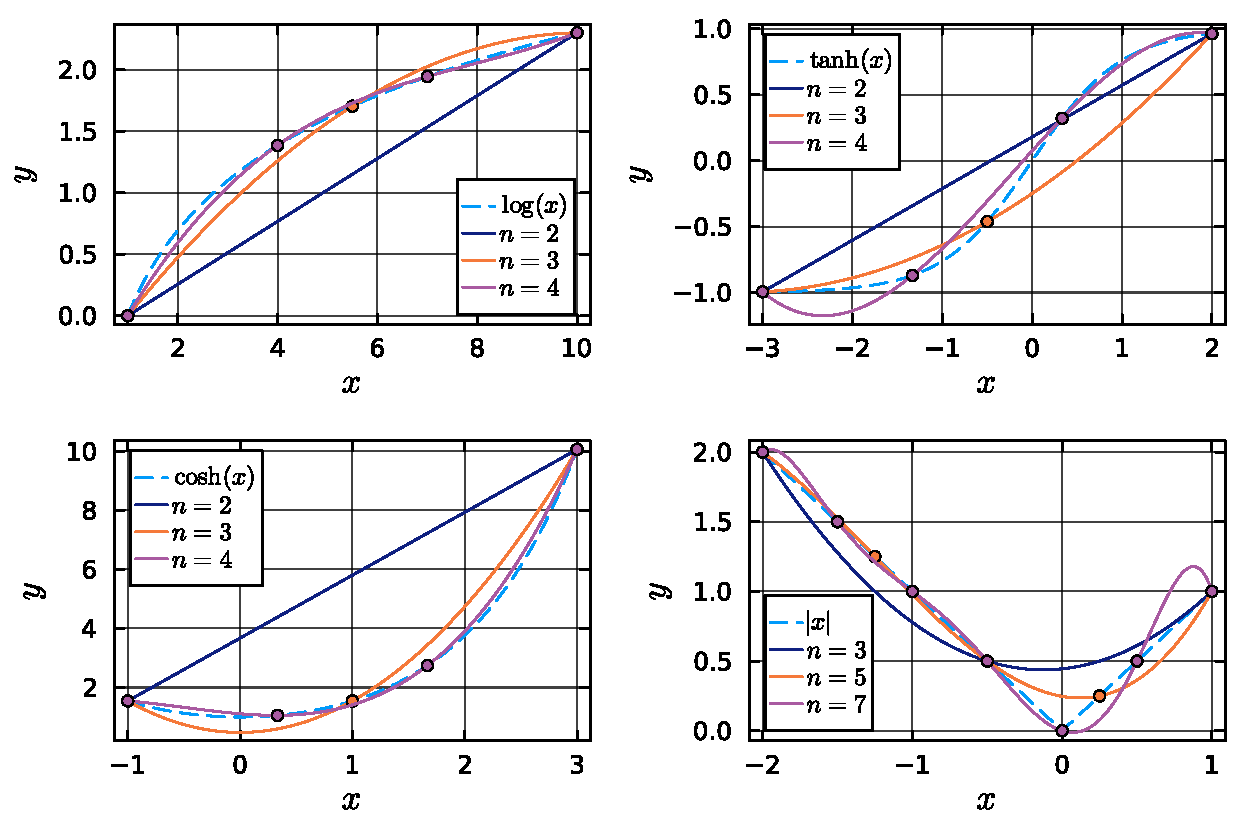
\includegraphics[width=0.8\textwidth]{4221.pdf}
    \caption{Grafici delle funzioni interpolanti per i vari casi.}
    \label{fig:es4_2_2_1}
\end{figure}

Come si può notare, all'aumentare del numero di nodi l'interpolazione migliora. Il grafico della funzione $|x|$
però richiede un numero di nodi maggiore per essere interpolato con una certa accuratezza, ciò è dovuto alla
non derivabilità della funzione in $x=0$. Il problema è che si sta cercando di interpolare una funzione
non derivabile con un polinomio, che notoriamente è derivabile in ogni punto.

\subsection{Esercizi 4.4.1, 4.4.2}
1. Scrivi un programma che implementi la formula baricentrica dell'interpolazione di Lagrange 
per il caso particolare dei nodi di Chebyshev, utilizzando i risultati analitici per i pesi. 
Verifica la correttezza della tua implementazione confrontandola con la routine per nodi generici. \\

2. (a) Per ciascun caso sotto riportato, calcola il polinomio interpolante usando $n$ nodi di Chebyshev di 
seconda specie in $[-1,1]$ per $n=4,8,12,\ldots,60$. Per ogni valore di $n$, calcola l'errore in norma $\infty$ 
(ossia, $||f-p||_\infty=\max_{x\in[-1,1]} |p(x)-f(x)|$ valutato su almeno 4000 valori di $x$). 
Utilizzando una scala log-lineare, rappresenta graficamente l'errore in funzione di $n$ e determina una 
buona approssimazione della costante $K$. \\
- $f(x) = 1/(25x^2+1)$  \\ 
- $f(x) = \tanh(5 x+2)$ \\ 
- $f(x) = \cosh(\sin x)$ \\ 
- $f(x) = \sin(\cosh x)$  \\

(b) Realizza un grafico analogo utilizzando $n$ punti equidistanti per l'interpolazione.

\subsubsection{Soluzione}
\paragraph{(1) } Si è implementata la formula baricentrica dell'interpolazione di Lagrange per il caso
particolare dei nodi di Chebyshev, e la si è testata nell'esercizio 4.4.2, confrontandola con il caso di 
nodi equidistanti. \\
\paragraph{(2a) } Il calcolo dell'errore in norma $\infty$ è stato effettuato con un passo di campionamento
sulle $x$ pari a $0.0005$, in modo da ottenere 4000 punti tra $-1$ e $1$. Si riportano in figura 
\ref{fig:es4_4_2_1} a sinistra i grafici dell'errore in norma $\infty$ in funzione di $n$, 
per i casi delle varie funzioni.
\begin{figure}[!ht]
    \begin{minipage}[b]{0.50\textwidth}
        \centering
        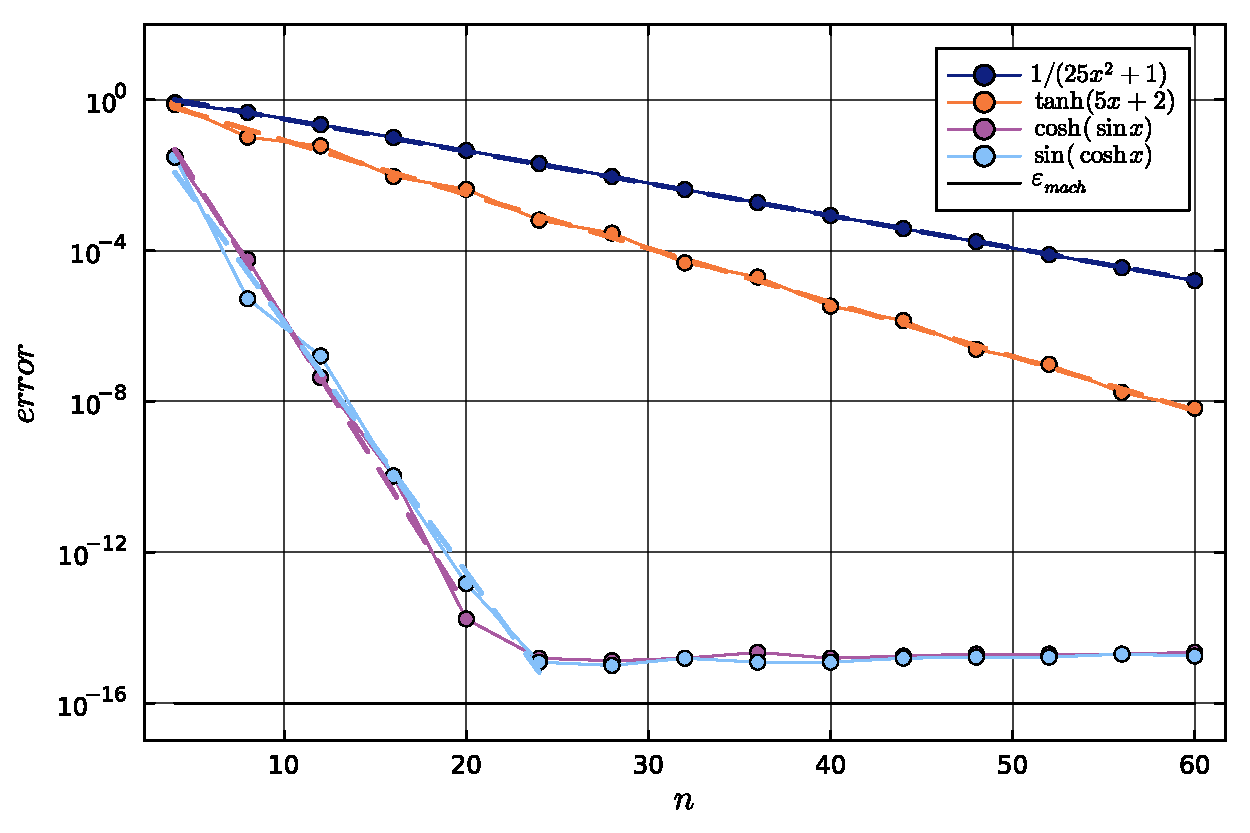
\includegraphics[width=0.9\textwidth]{4421.pdf}
        \caption*{}
    \end{minipage}
    \begin{minipage}[b]{0.50\textwidth}
        \centering
        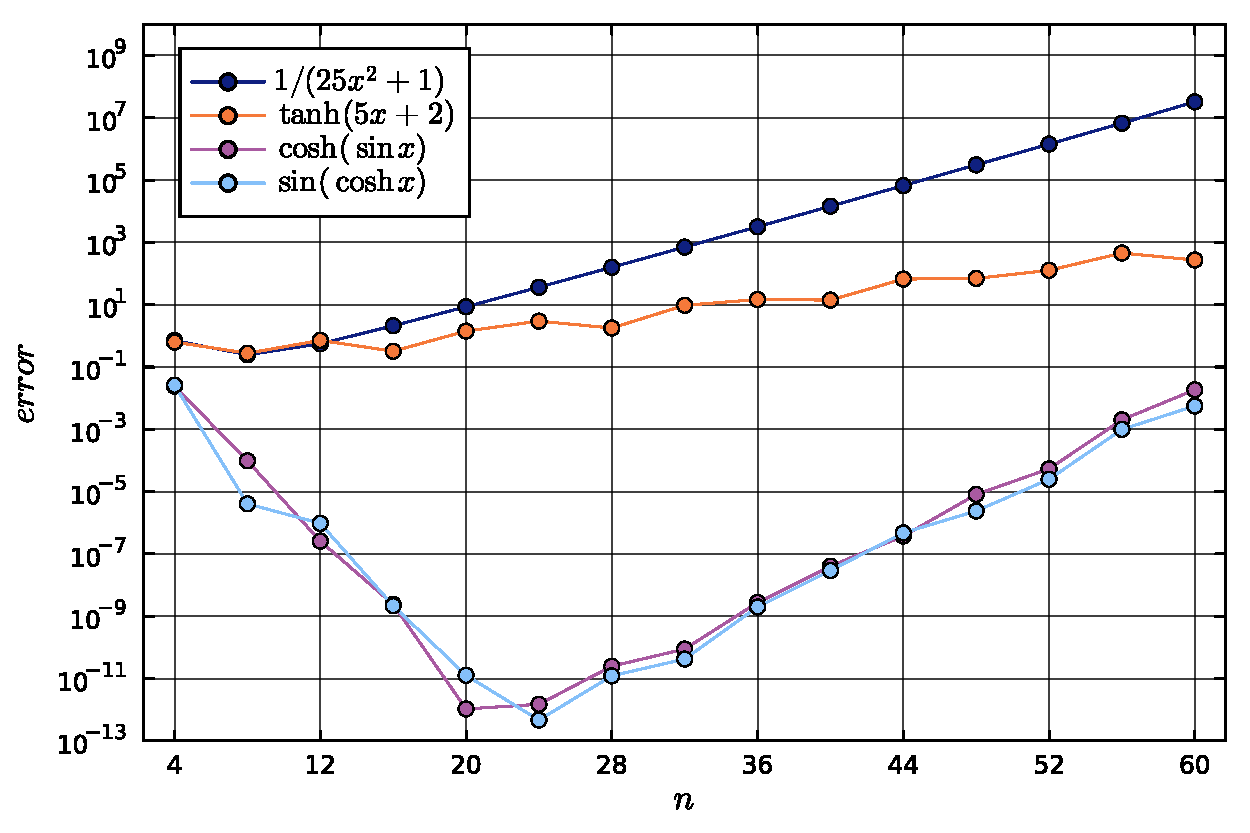
\includegraphics[width=0.9\textwidth]{4422.pdf}
        \caption*{}
    \end{minipage}
    \caption{Errori per nodi di Chebyshev (sinistra) e nodi equidistanti (destra).}
    \label{fig:es4_4_2_1}
\end{figure}

La prima osservazione che si può fare è che l'errore in norma $\infty$ decresce all'aumentare di $n$,
come ci si aspetta data la scelta dei nodi di Chebyshev. La seconda osservazione è che l'errore decresce
con un andamento esponenziale, fino ad arrestare la sua discesa intorno al valore di $\epsilon_{mach} = 10^{-16}$. \\
La relazione che ha consentito di stimare la costante $K$ è la seguente:
\begin{equation}
    |p(x)-f(x)| = C \cdot K^(-n), \qquad \log_{10}|p(x)-f(x)| = \log_{10}(C) + n(-\log_{10}(K)),
\end{equation}
dove si è scelto di linearizzare i dati con il logaritmo per poter stimare la costante $K$ tramite
il coefficiente angolare della retta di regressione. I fit sono stati eseguiti scartando i punti corrispondenti
a errori minori di $10^{-16}$, e in figura \ref{fig:es4_4_2_1} sono rappresentati dalle linee tratteggiate. \\
Si riportano i valori di $K$ ottenuti per le varie funzioni:
\begin{itemize}
    \item $f_1(x) = 1/(25x^2+1)$: $K = 1.217$.
    \item $f_2(x) = \tanh(5 x+2)$: $K = 1.391$.
    \item $f_3(x) = \cosh(\sin x)$: $K = 5.704$.
    \item $f_4(x) = \sin(\cosh x)$: $K = 4.598$.
\end{itemize}

\paragraph{(2b) } Si è ripetuto lo stesso procedimento con i nodi equidistanti, e si riportano in 
figura \ref{fig:es4_4_2_1} a destra
i grafici dell'errore in norma $\infty$ in funzione di $n$, per i vari casi.
Come atteso, l'errore in norma $\infty$ non decresce globalmente all'aumentare di $n$. Per le prime due funzioni
l'errore è crescente fin dall'inizio, mentre per le ultime due funzioni l'errore decresce fino a un certo punto, 
per tornare a crescere successivamente. È un comportamento noto come \textit{fenomeno di Runge}, ed è 
dovuto alla scelta dei nodi equidistanti. \\ 

\subsection{Esercizio 4.4.3}
I punti di Chebyshev possono essere utilizzati anche quando l'intervallo di interpolazione è $[a,b]$ 
invece di $[-1,1]$, tramite un opportuno cambiamento di variabile. 
Traccia il polinomio interpolante di $f(z) = \cosh(\sin z)$ su $[0,2\pi]$ utilizzando $n=40$ nodi di Chebyshev.

\subsubsection{Soluzione}
Il cambio di variabile utilizzato per passare da $[-1,1]$ a $[a,b]$ è il seguente:
\begin{equation}
    \label{eq:change_of_var1}
    z = \psi(x) = a + (b-a) \frac{x+1}{2},
\end{equation}
dove $x$ è il nodo di Chebyshev. \\
L'algoritmo implementato tiene conto di questo cambio di variabile. In particolare si sono calcolati i nodi 
di Chebyshev, li si è trasformati con \ref{eq:change_of_var1} e poi si è calcolato il polinomio nei nuovi punti con 
i soliti pesi. Si riporta in figura \ref{fig:es4_4_3_1} 
il grafico ottenuto con $n=40$ nodi di Chebyshev, per la funzione $f(z) = \cosh(\sin z)$ su $[0,2\pi]$.
\begin{figure}[!ht]
    \centering
    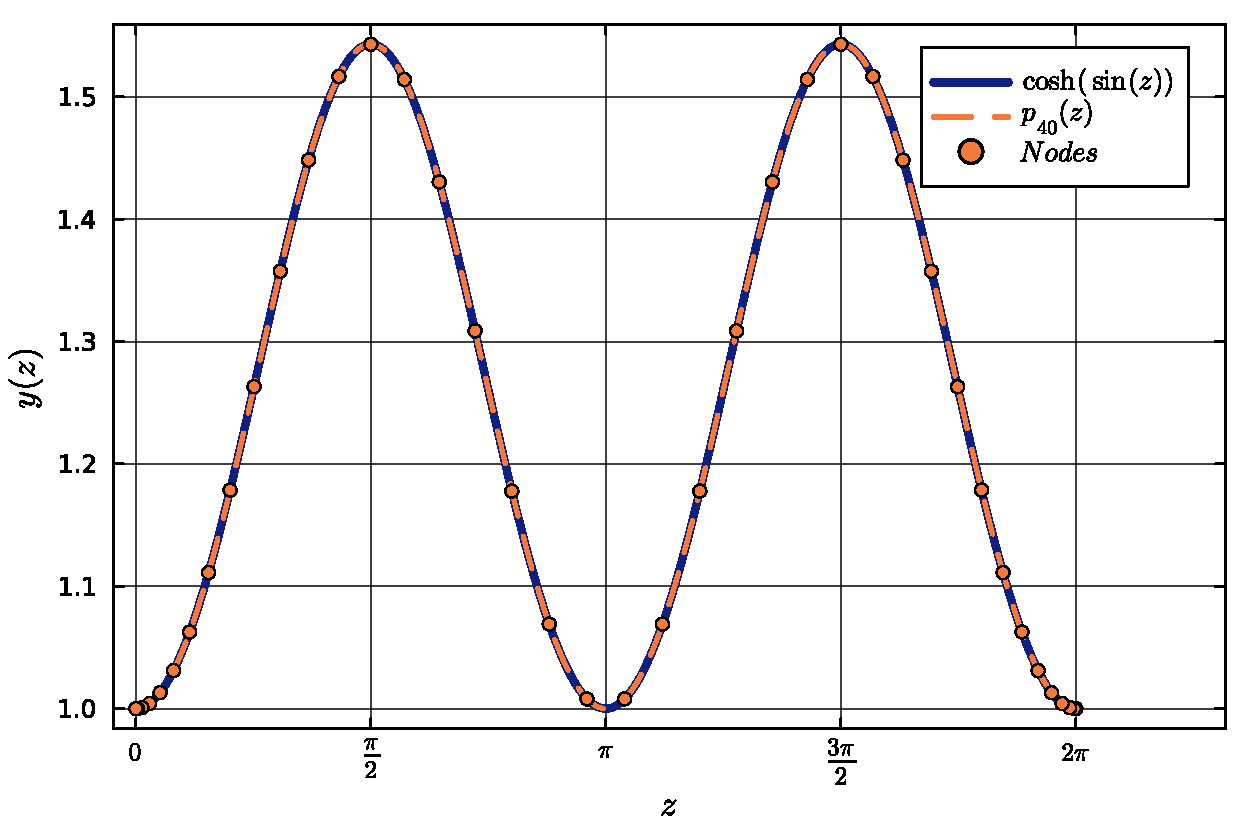
\includegraphics[width=0.7\textwidth]{4431.pdf}
    \caption{$f(z) = \cosh(\sin z)$ su $[0,2\pi]$ con $n=40$ nodi di Chebyshev.}
    \label{fig:es4_4_3_1}
\end{figure}

\subsection{Esercizio 4.4.4}
Siano $x_1,\ldots,x_n$ i punti di Chebyshev standard. Questi vengono mappati nella variabile $z$ come 
$z_i=\phi(x_i)$ per ogni $i$, dove $\phi$ è una trasformazione sulla retta reale. Supponiamo che $f(z)$ 
sia una funzione data, il cui dominio è l'intera retta reale. Allora i valori della funzione $y_i=f(z_i)$ 
possono essere associati ai nodi di Chebyshev $x_i$, portando a un polinomio interpolante $p(x)$. 
Questo implica a sua volta una funzione interpolante sulla retta reale, definita come
\begin{equation}
    q(z)=p\bigl(\phi^{-1}(z)\bigr) = p(x)\,.
\end{equation}
Implementa questa idea per tracciare un interpolante di $f(z)=(z^2-2z+2)^{-1}$ usando $n=30$. 
Il tuo grafico deve mostrare $q(z)$ valutato in 1000 punti equispaziati in $[-6,6]$, 
con marcatori sui valori nodali (quelli che ricadono nella finestra $[-6,6]$). \\
Suggerimento: se preferisci evitare di gestire potenziali infiniti considera l'uso dei nodi di Chebyshev di 
prima specie.

\subsubsection{Soluzione}
Il cambio di variabile utilizzato è il seguente: 
\begin{equation}
    \label{eq:change_of_var2}
    z = \phi(x) = \frac{2x}{1 - x^2},
\end{equation}
La funzione Julia implementata tiene conto di questo cambio di variabile. In particolare calcola i nodi 
di Chebyshev del secondo tipo nell'intervallo $[-1, 1]$, che vengono denotati come $x_i$, e li trasformati 
con \ref{eq:change_of_var2} per ottenere i nodi di Chebyshev $z_i$, ora distribuiti sull'intera retta reale. 
I punti per i quali passa il polinomio vengono indicati con $y_i = f(z_i)$. \\
La funzione restituisce il polinomio interpolante $q(z)$. Per calcolarlo si utilizza la trasformazione inversa
di \ref{eq:change_of_var2} portare i punti $z$ in cui verrà calcolato il polinomio $q$ nell'intervallo $[-1, 1]$.
A questo punto avviene l'interpolazione con i nodi di Chebyshev $x_i$ e i valori $y_i$, e così il polinomio
restituito interpola su tutto l'asse reale avendo calcolato l'interpolazione su un intervallo finito. \\
Si riporta in figura \ref{fig:es4_4_4_1} il grafico della funzione $f(z)=(z^2-2z+2)^{-1}$ e della sua interpolazione
con $n=30$ nodi di Chebyshev. Per motivi di rappresentazione grafica l'intervallo è stato limitato a $[-6, 6]$, 
si noti infatti che il numero di nodi in grafico è pari a venti: i dieci restanti sono al di fuori dell'intervallo.
\begin{figure}[!ht]
    \centering
    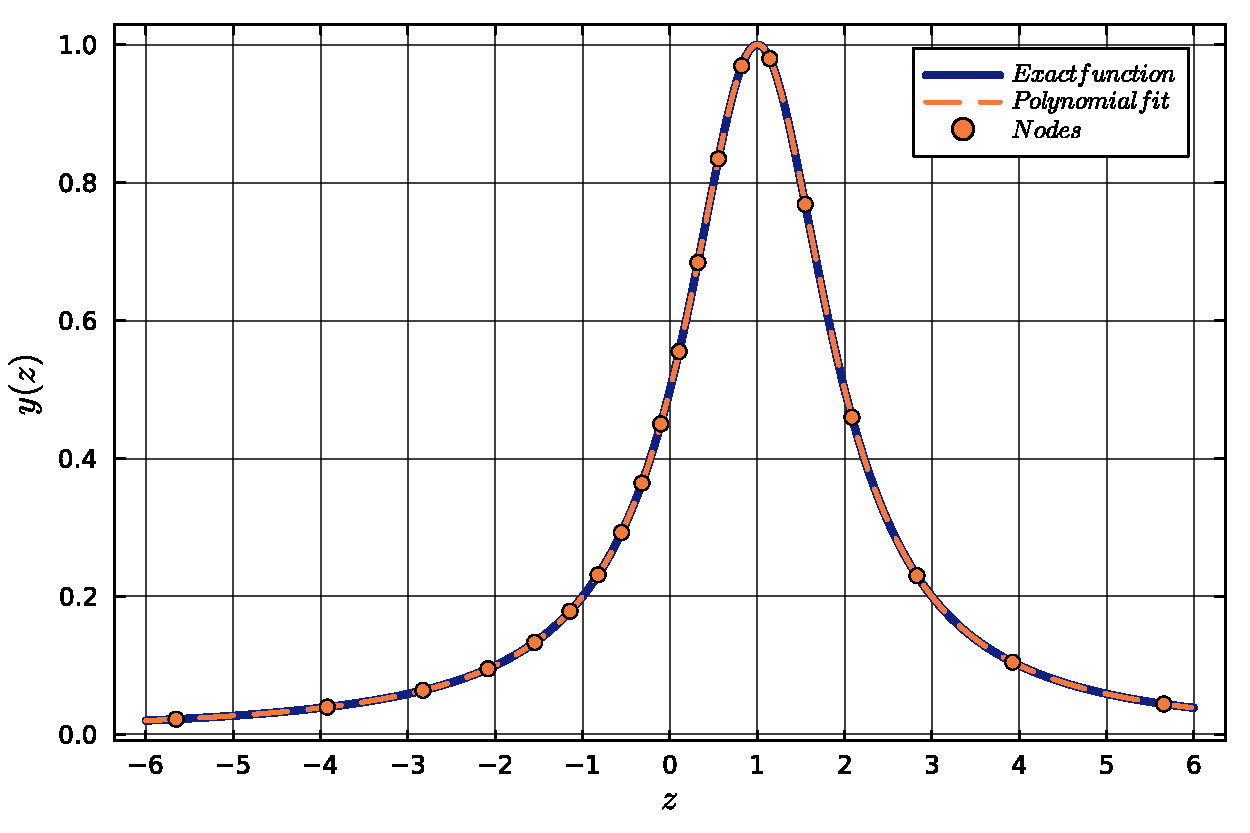
\includegraphics[width=0.7\textwidth]{4441.pdf}
    \caption{$f(z)=(z^2-2z+2)^{-1}$ e relativa interpolazione con $30$ nodi di Chebyshev.}
    \label{fig:es4_4_4_1}
\end{figure}

\subsection{Esercizio 4.6.1} 
Ognuna delle seguenti funzioni è 2-periodica. Scrivi una funzione che esegua l'interpolazione trigonometrica 
su $[-1,1]$ e traccia la funzione insieme ai suoi interpolanti trigonometrici per $n=3,6,9$. 
Poi, per $n=2,3,\ldots,30$, calcola l'errore in norma $\infty$ dell'interpolante trigonometrico campionando 
in almeno $1000$ punti, e realizza un grafico di convergenza in scala semi-logaritmica. \\
(a) $f(x) = e^{\sin (2\pi x)}\qquad$ \\
(b) $f(x) = \log [2+ \sin (3 \pi x ) ]\qquad$ \\
(c) $f(x) = \cos^{12}[\pi (x-0.2)]$ \\

\subsubsection{Soluzione}
Ai fini dell'esercizio si è sviluppata una funzione Julia che calcola l'interpolazione trigonometrica
su un intervallo $[-1, 1]$ per una funzione $f(x)$, e restituisce il polinomio interpolante. Dato che le funzioni
sono 2-periodiche le si è interpolate correttamente sull'intervalo $[-1, 1]$. Per poter interpolare funzioni 
T-periodiche bisogna inserire nell'algoritmo un cambio di variabile, proprio come per l'esercizio 4.4.3.
\paragraph{(a) } Si riporta in figura \ref{fig:es4_6_1_1} il grafico della funzione $f(x) = e^{\sin (2\pi x)}$
e dei suoi interpolanti trigonometrici per $n=3,6,9$. A fianco si riporta anche il grafico 
dell'errore in norma $\infty$ dell'interpolante trigonometrica al variare del numero di nodi, avendo campionato 
in 1000 punti l'intervallo.
\begin{figure}[!ht]
    \centering
    \begin{minipage}[b]{0.47\textwidth}
        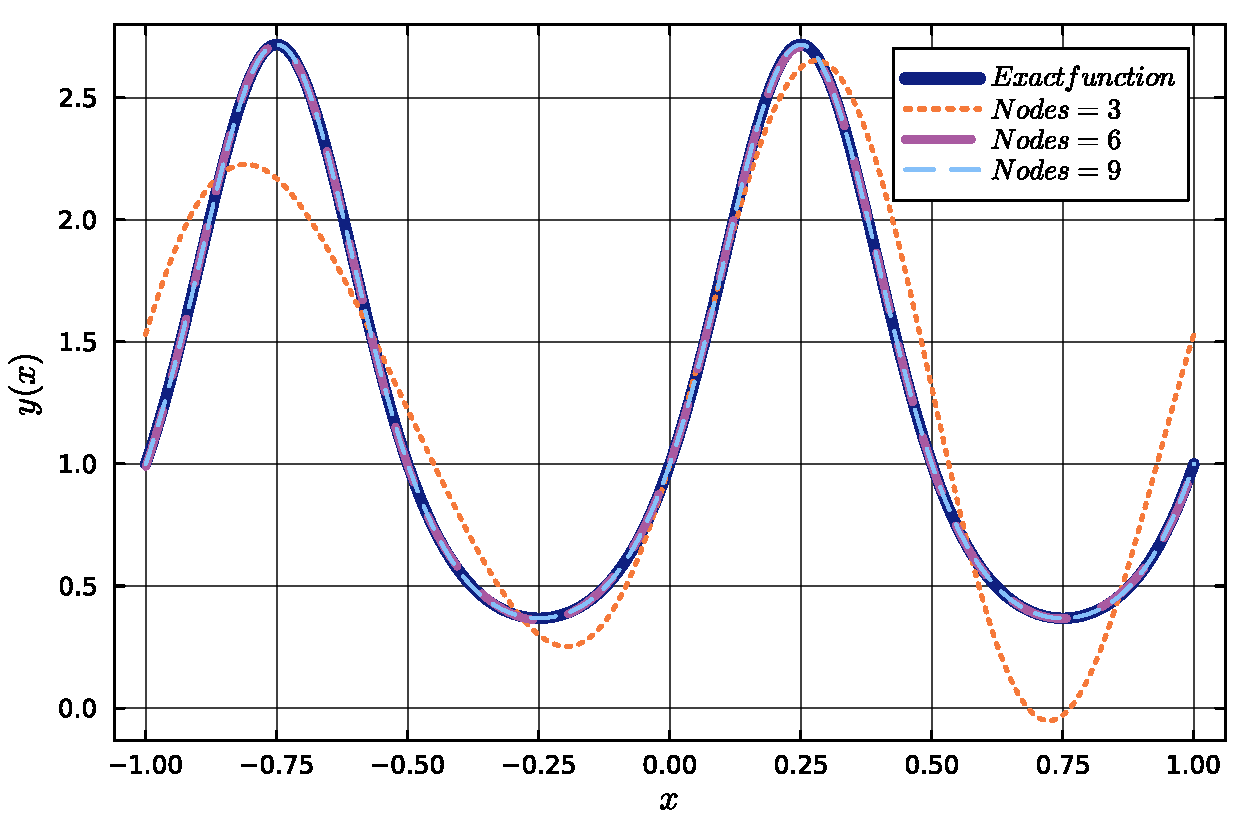
\includegraphics[width=\textwidth]{4611.pdf}
    \end{minipage}
    \hspace{0.5cm}
    \begin{minipage}[b]{0.47\textwidth}
        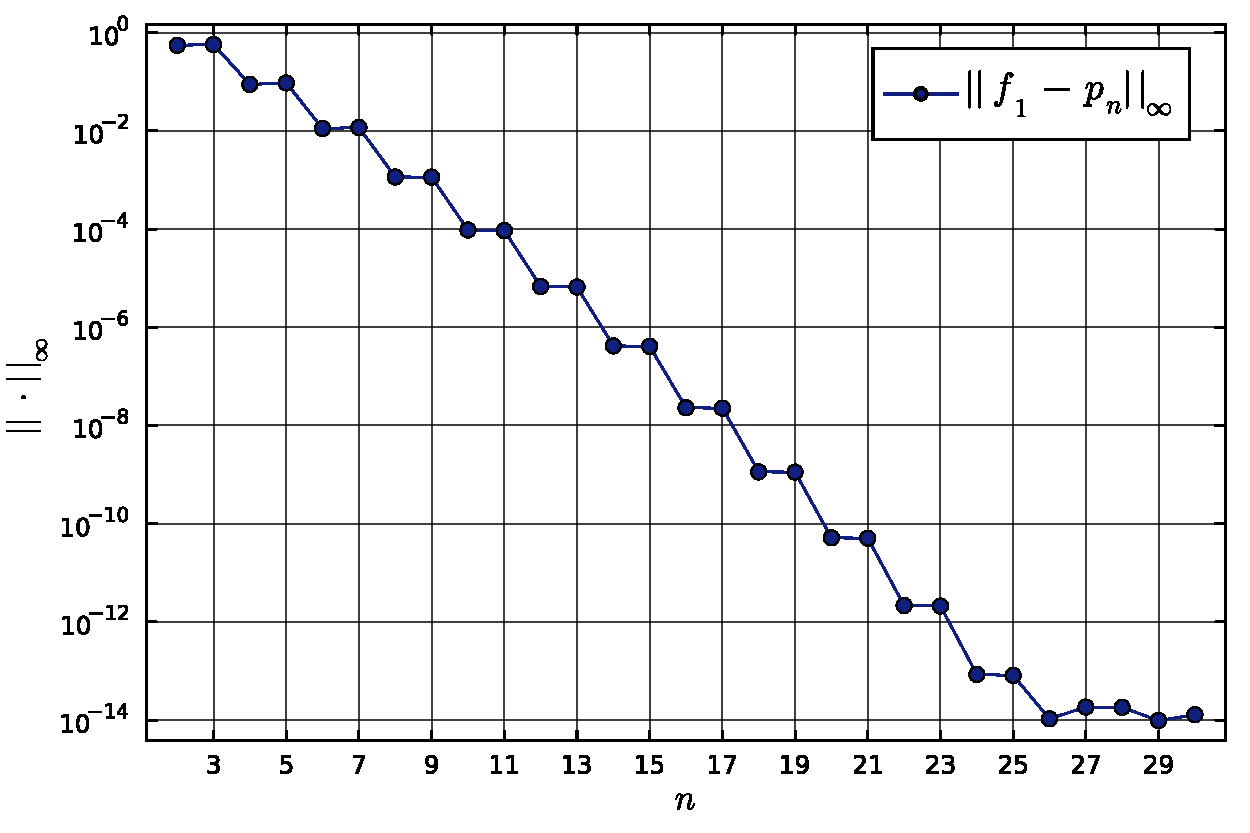
\includegraphics[width=\textwidth]{4612.pdf}
    \end{minipage}
    \caption{Studio delle interpolazioni trigonometriche per la funzione $f(x) = e^{\sin (2\pi x)}$.}
    \label{fig:es4_6_1_1}
\end{figure}
\paragraph{(b) } Si riporta in figura \ref{fig:es4_6_1_2} il grafico della funzione $f(x) = \log [2+ \sin (3 \pi x ) ]$
e dei suoi interpolanti trigonometrici per $n=3,6,9$. A fianco si riporta anche il grafico
dell'errore in norma $\infty$ dell'interpolante trigonometrica al variare del numero di nodi, avendo campionato
in 1000 punti l'intervallo.
\begin{figure}[!ht]
    \centering
    \begin{minipage}[b]{0.47\textwidth}
        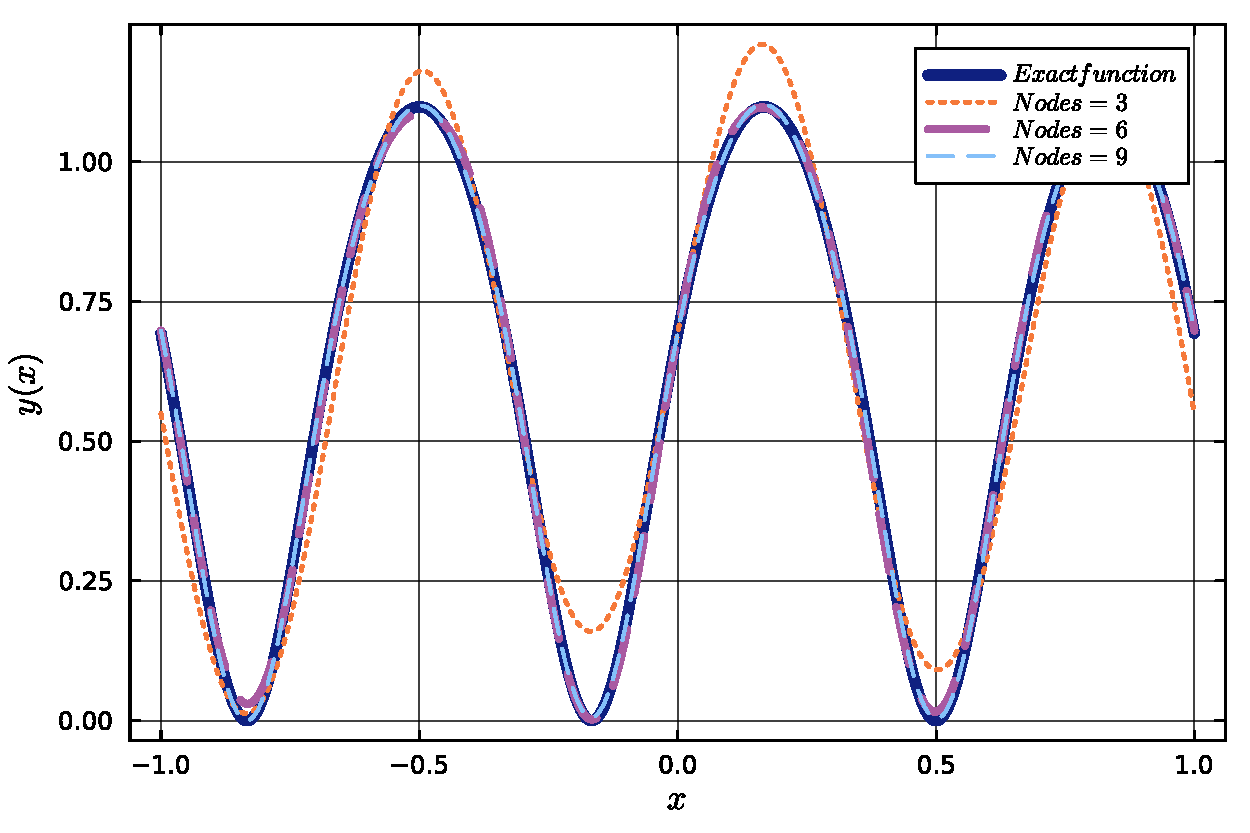
\includegraphics[width=\textwidth]{4613.pdf}
    \end{minipage}
    \hspace{0.5cm}
    \begin{minipage}[b]{0.47\textwidth}
        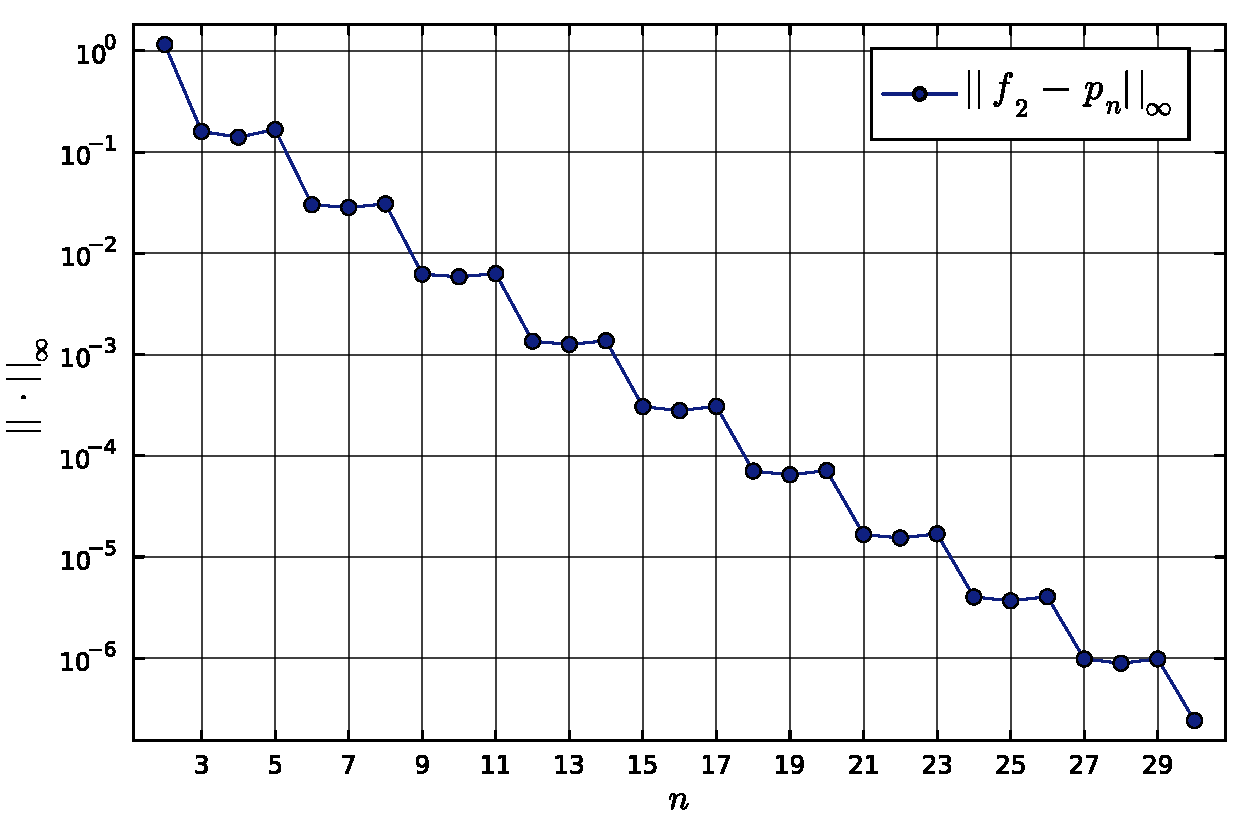
\includegraphics[width=\textwidth]{4614.pdf}
    \end{minipage}
    \caption{Studio delle interpolazioni trigonometriche per la funzione $f(x) = \log [2+ \sin (3 \pi x ) ]$.}
    \label{fig:es4_6_1_2}
\end{figure}

\paragraph{(c) } Si riporta in figura \ref{fig:es4_6_1_3} il grafico della funzione $f(x) = \cos^{12}[\pi (x-0.2)]$
e dei suoi interpolanti trigonometrici per $n=3,6,9$. A fianco si riporta anche il grafico
dell'errore in norma $\infty$ dell'interpolante trigonometrica al variare del numero di nodi, avendo campionato
in 1000 punti l'intervallo.
\begin{figure}[!ht]
    \centering
    \begin{minipage}[b]{0.47\textwidth}
        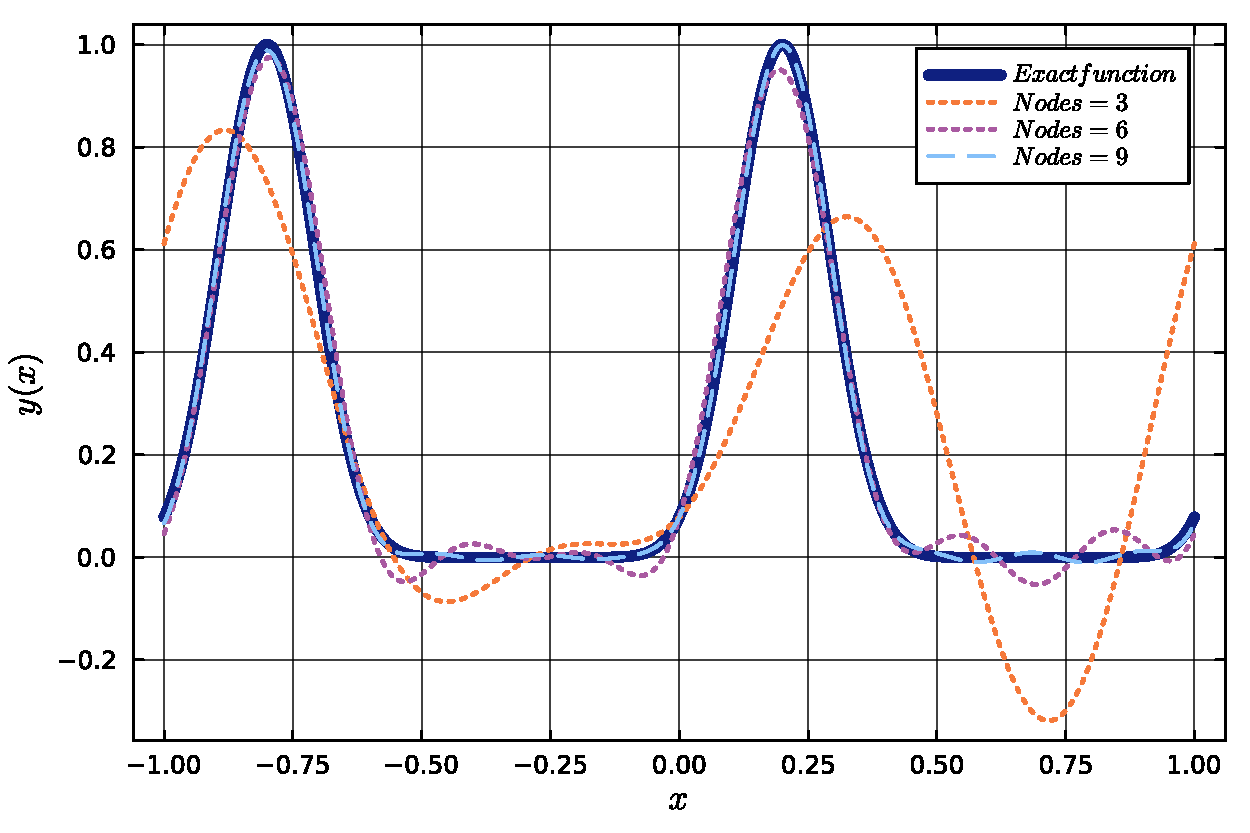
\includegraphics[width=\textwidth]{4615.pdf}
    \end{minipage}
    \hspace{0.5cm}
    \begin{minipage}[b]{0.47\textwidth}
        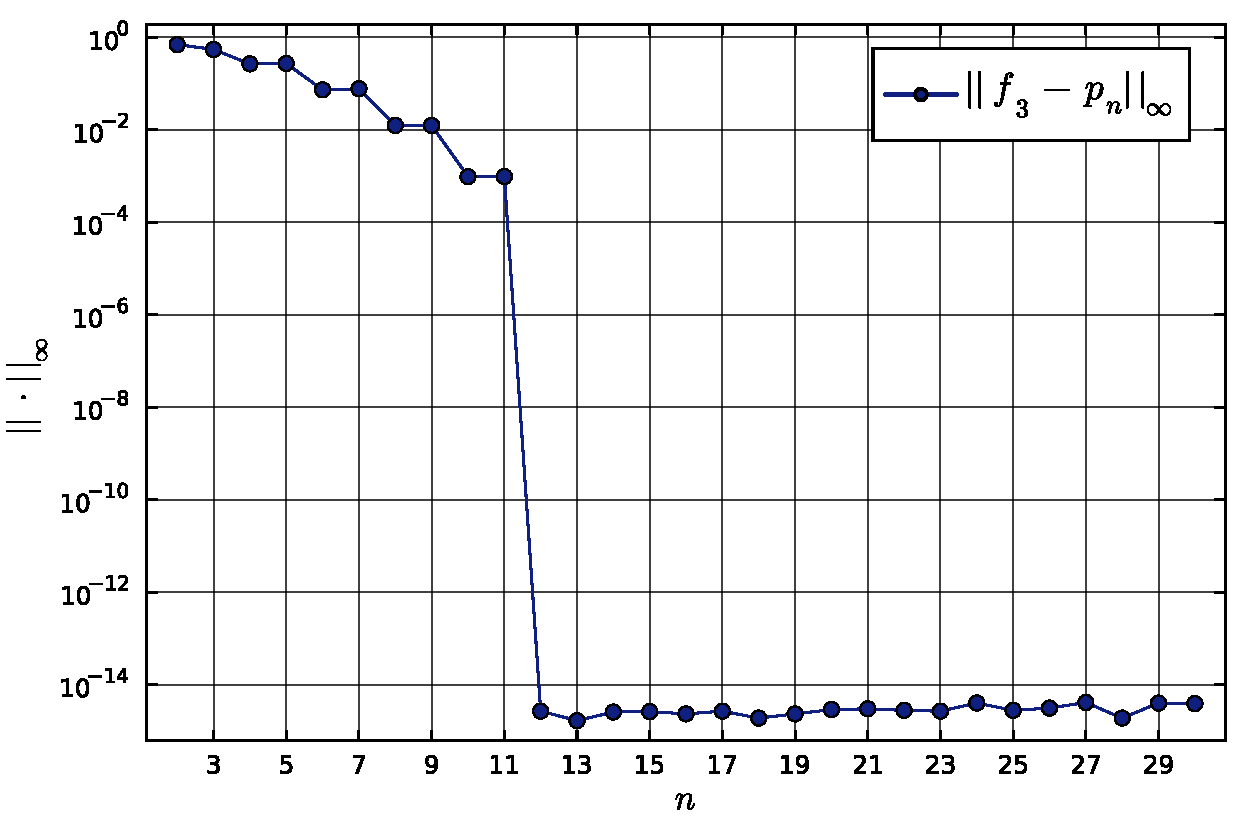
\includegraphics[width=\textwidth]{4616.pdf}
    \end{minipage}
    \caption{Studio delle interpolazioni trigonometriche per la funzione $f(x) = \cos^{12}[\pi (x-0.2)]$.}
    \label{fig:es4_6_1_3}
\end{figure}

\paragraph{Osservazioni}
Si osserva che l'errore in norma $\infty$ diminuisce all'aumentare del numero di nodi in tutti e tre i casi, 
confermando la convergenza dell'interpolazione trigonometrica. In generale l'errore non diminuisce mai oltre
il valore di $10^{-14}$ per motivazioni legate alla rappresentazione numerica. È interessante notare che 
in tutti e tre i casi l'errore ha un andamento a gradino. Questo fenomeno mostra che l'aggiunta di nodi 
non sempre migliora l'accuratezza dell'interpolazione, anche se globalmente l'errore diminuisce. \\
Curioso infine è il comportamento dell'errore per la terza funzione, in cui per $n = 12$ si osserva una
diminuizione drastica dell'errore. Sulle ragioni di questo fatto si è avanzata una spiegazione. 
Osservando il grafico \ref{fig:es4_6_1_3} si nota che all'aumento di $n$ le zone che sono peggio approssimate sono 
quelle di appiattimento della funzione, e cioè sono quelle che contribuiscono all'errore, calcolato 
come il massimo della distanza tra la funzione e il polinomio interpolante, su tutto l'intervallo. \\
La figura \ref{fig:es4_6_1_4} è un ingrandimento di figura \ref{fig:es4_6_1_3} nella regione interessata e 
si osserva che per $n=12$ il polinomio interpolante si appiattisce definitivamente, con la conseguente 
riduzione dell'errore.
\begin{figure}[!ht]
    \centering
    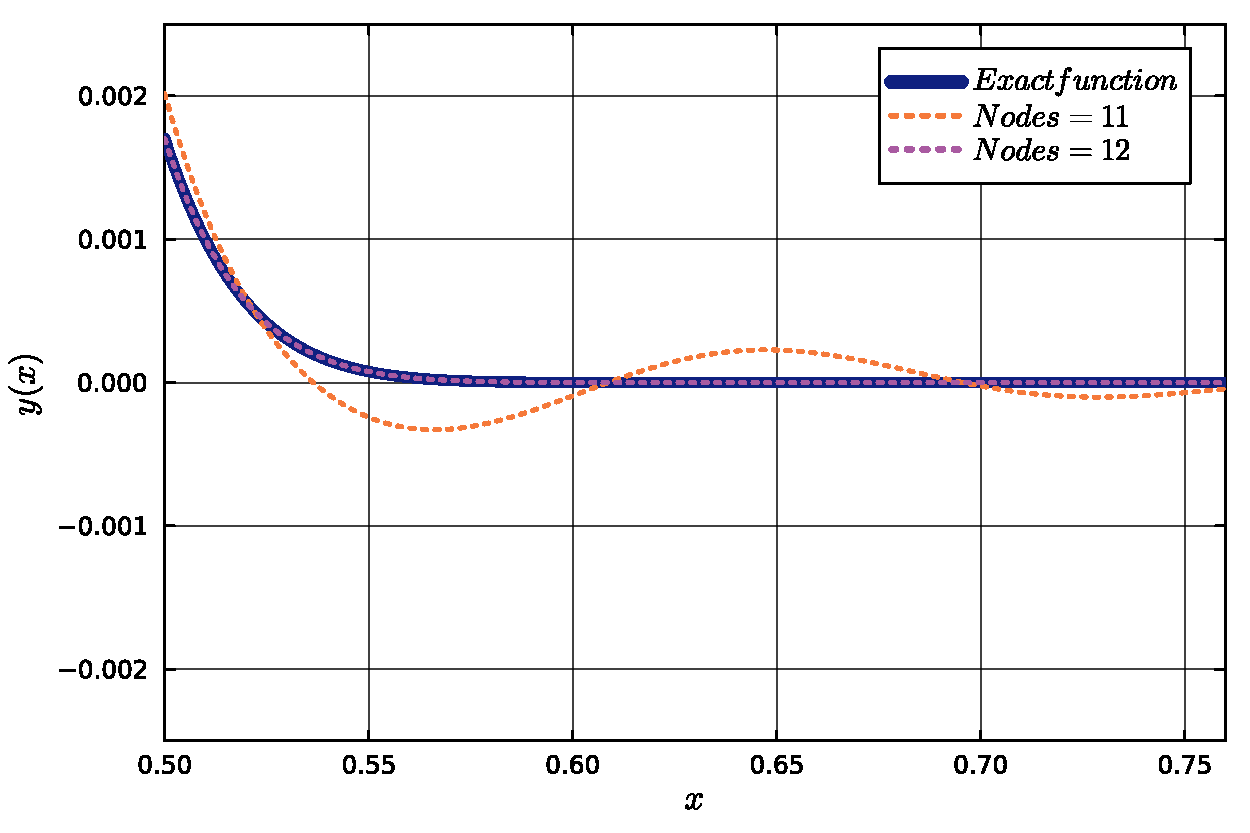
\includegraphics[width=0.8\textwidth]{4617.pdf}
    \caption{Ingrandimento della figura \ref{fig:es4_6_1_3} nella regione di appiattimento della funzione.}
    \label{fig:es4_6_1_4}
\end{figure}

\section{Integrazione numerica}
\subsection{Esercizi 5.1.1, 5.1.2}
1. Scrivi un programma che implementi la regola del trapezio composta per un intervallo generico $[a,b]$. \\
2. Per ciascuno dei seguenti integrali, utilizza la regola del trapezio per stimare il valore dell'integrale 
con $m=10\cdot 2^k$ nodi, per $k=1,2,\ldots,10$. Per ogni caso, rappresenta in scala log-log l'errore in funzione 
di $m$ e verifica se la convergenza è di secondo ordine.

\begin{itemize}
    \item[(a)] $\displaystyle \int_0^1 x\log(1+x)\, dx = \frac{1}{4}$
    \item[(b)] $\displaystyle \int_0^1 x^2 \tan^{-1}x\, dx = \frac{\pi-2+2\log 2}{12}$
    \item[(c)] $\displaystyle \int_0^{\pi/2}e^x \cos x\, dx = \frac{e^{\pi/2}-1}{2}$
    \item[(d)] $\displaystyle \int_0^1 \frac{\tan^{-1}(\sqrt{2+x^2})}{(1+x^2)\sqrt{2+x^2}}\,dx = \frac{5\pi^2}{96}$
    \item[(e)] $\displaystyle \int_0^1 \sqrt{x} \log(x) \, dx = -\frac{4}{9}$ \\
        \textit{Suggerimento:} Sebbene l'integranda abbia limite zero per $x\to 0$, non può essere valutata direttamente in $x=0$. 
        Una possibilità è iniziare l'integrale da $x=\epsilon_{\rm mach}$. In alternativa, puoi definire una 
        funzione wrapper $g(x)$ che restituisce $g(0)=0$ e $g(x)=\sqrt{x}\log(x)$ altrimenti.
    \item[(f)] $\displaystyle \int_0^1 \sqrt{1-x^2}\, dx = \frac{\pi}{4}$
\end{itemize}

\subsubsection{Soluzione}
\paragraph{(1) } Si è implementata la regola del trapezio composta per un intervallo generico $[a,b]$,
e la si è testata nell'esercizio 5.1.2. \\
\paragraph{(2) } Si è calcolato l'integrale con la regola del trapezio per tutti i casi, al variare del numero di
nodi. Oltre alla rappresentazione grafica dell'errore, si sono rappresentate le derivate seconde dell'integranda,
in modo da poter verificare la convergenza di ordine secondo della regola del trapezio. La motivazione
di tale scelta è che l'errore della regola del trapezio scala al secondo ordine con il passo di campionamento,
ma ha per coefficiente la derivata seconda dell'integranda, calcolata in un certo $\xi$ appartenente all'intervallo
in considerazione. In formule:
\[
R_T(h) = -\frac{(b-a)^3 }{12}h^2 f''(\xi)
\]
Si riportano nelle figure \ref{fig:es5_1_2_1}, \ref{fig:es5_1_2_2}, \ref{fig:es5_1_2_3}, 
\ref{fig:es5_1_2_4}, \ref{fig:es5_1_2_5}, \ref{fig:es5_1_2_6} gli studi dei vari casi.

\begin{figure}[!ht]
    \centering
    \begin{minipage}[b]{0.47\textwidth}
        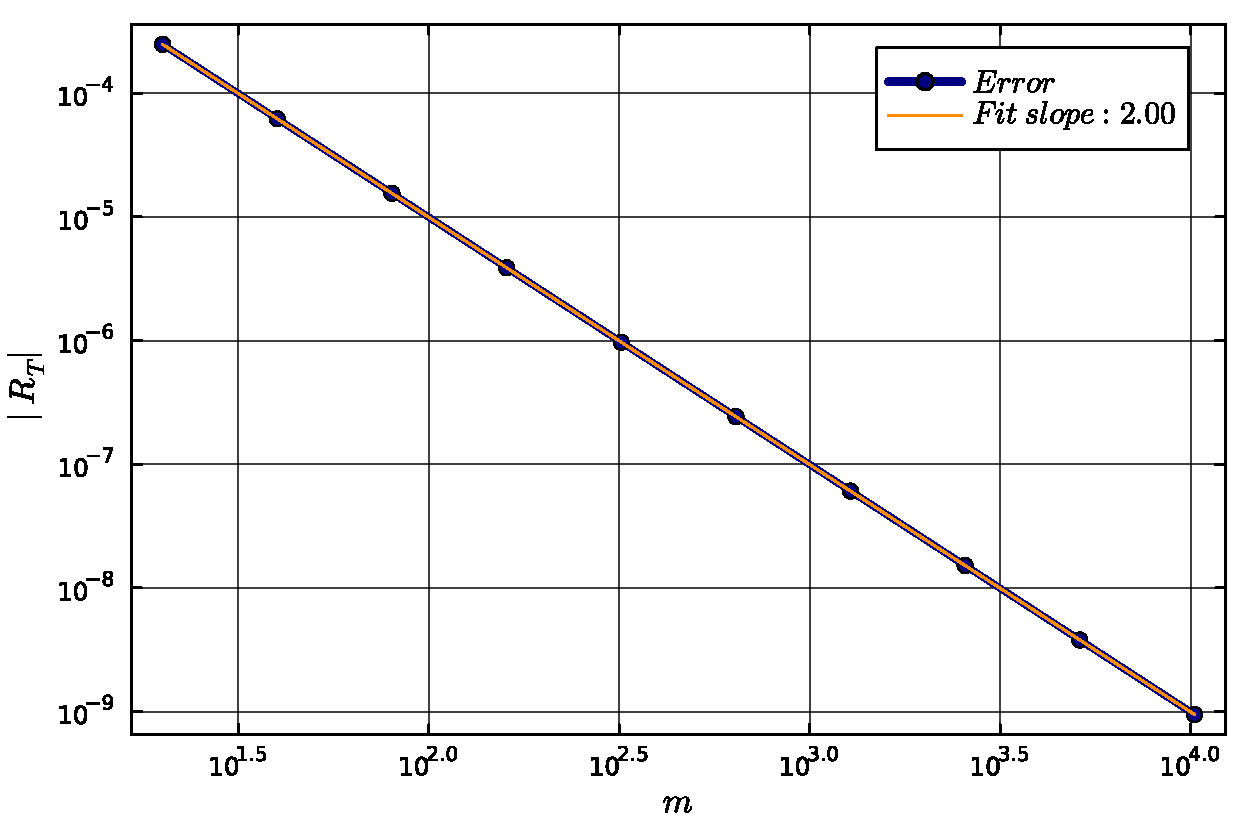
\includegraphics[width=\textwidth]{5121.pdf}
    \end{minipage}
    \hspace{0.5cm}
    \begin{minipage}[b]{0.47\textwidth}
        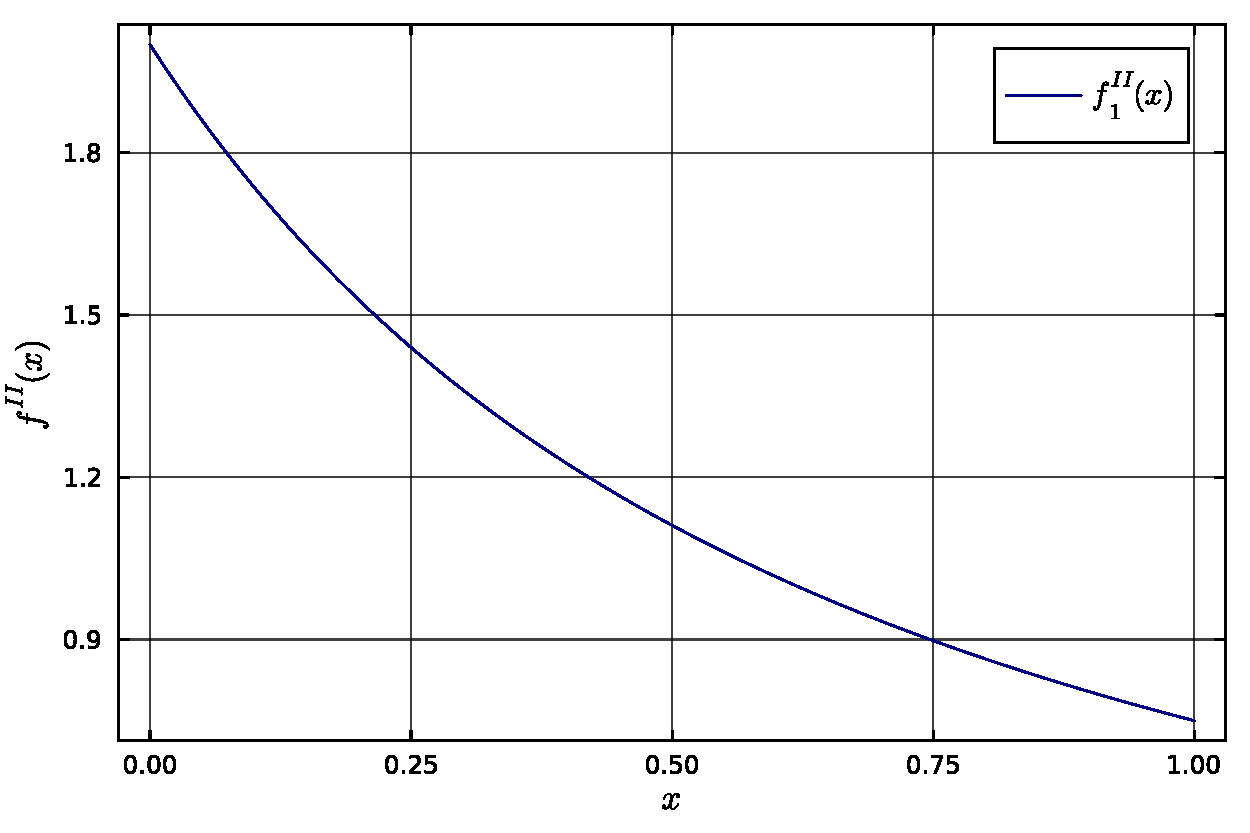
\includegraphics[width=\textwidth]{5121_2.pdf}
    \end{minipage}
    \caption{Studio della regola del trapezio per l'integrale $\int_0^1 x\log(1+x)\, dx$.}
    \label{fig:es5_1_2_1}
\end{figure}
\begin{figure}[!ht]
    \centering
    \begin{minipage}[b]{0.47\textwidth}
        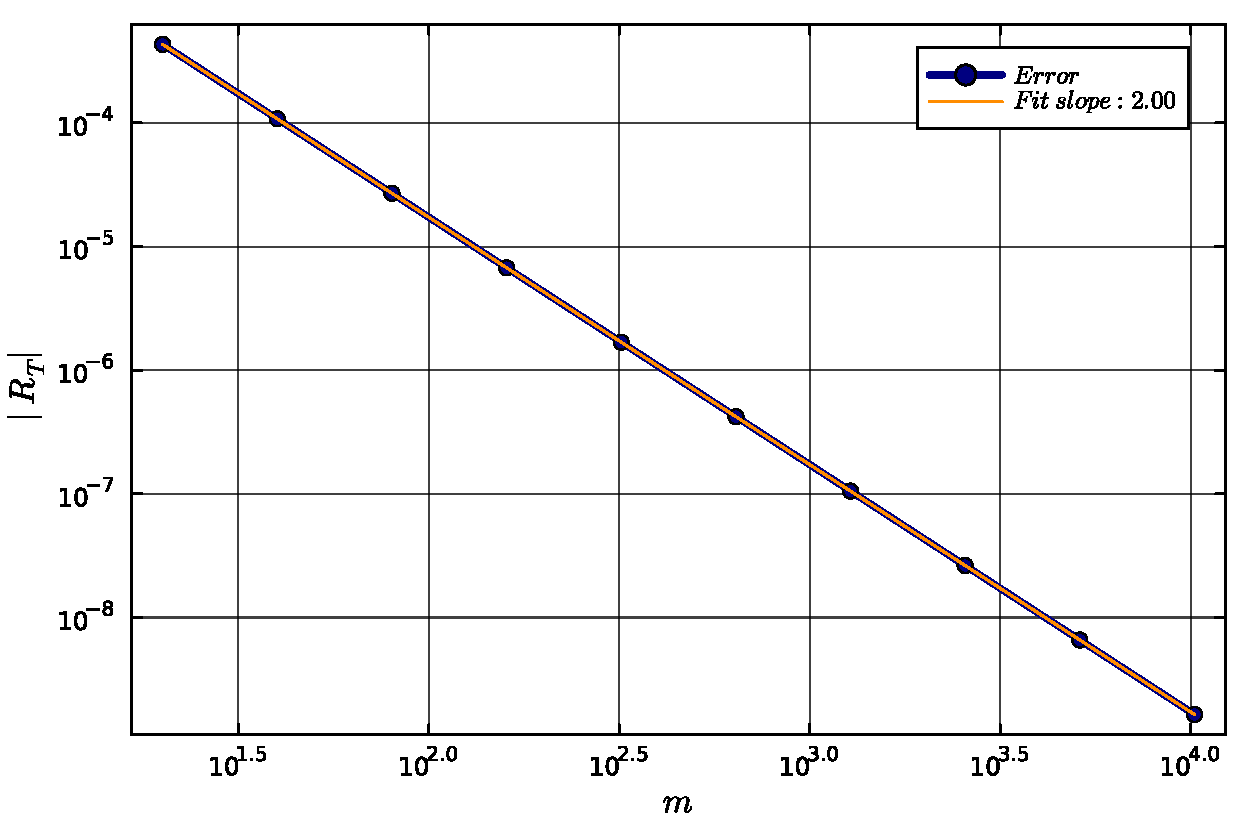
\includegraphics[width=\textwidth]{5122.pdf}
    \end{minipage}
    \hspace{0.5cm}
    \begin{minipage}[b]{0.47\textwidth}
        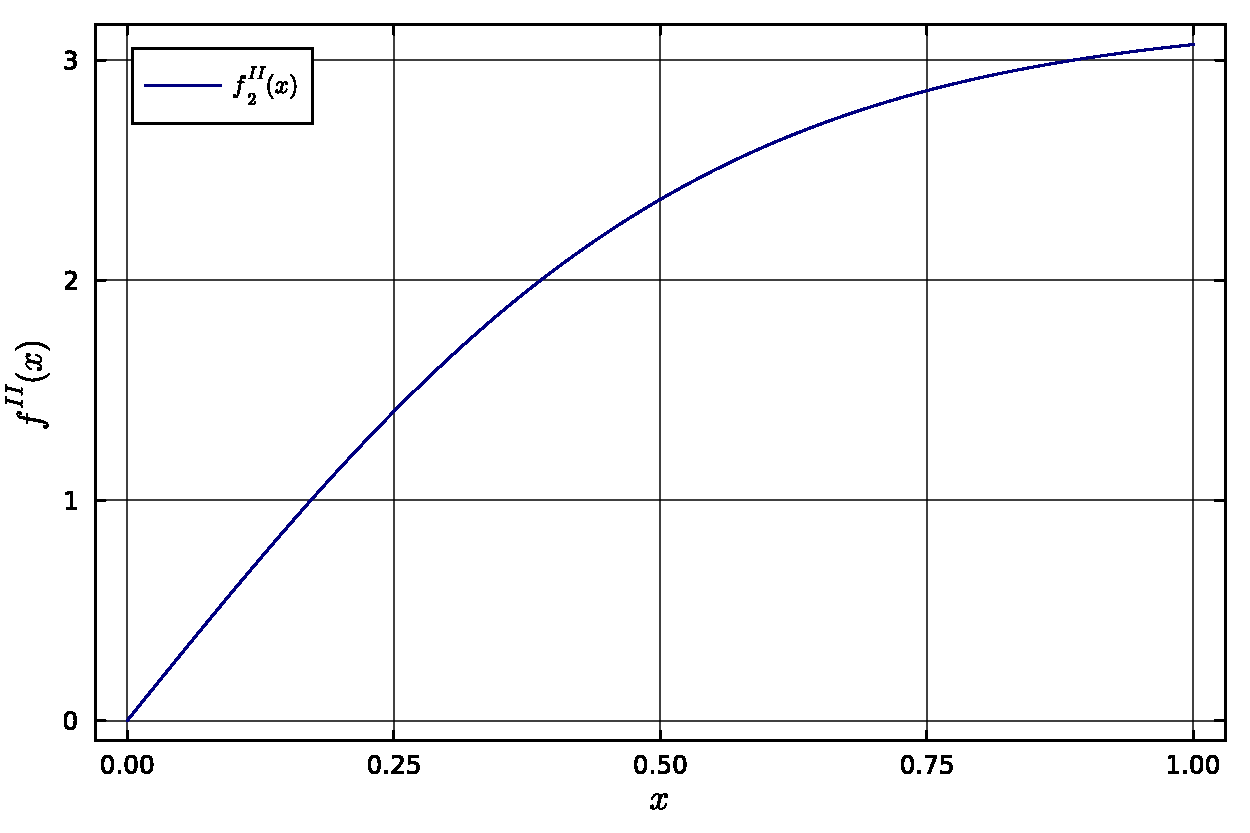
\includegraphics[width=\textwidth]{5122_2.pdf}
    \end{minipage}
    \caption{Studio della regola del trapezio per l'integrale $\int_0^1 x^2 \tan^{-1}x\, dx$.}
    \label{fig:es5_1_2_2}
\end{figure}
\begin{figure}[!ht]
    \centering
    \begin{minipage}[b]{0.47\textwidth}
        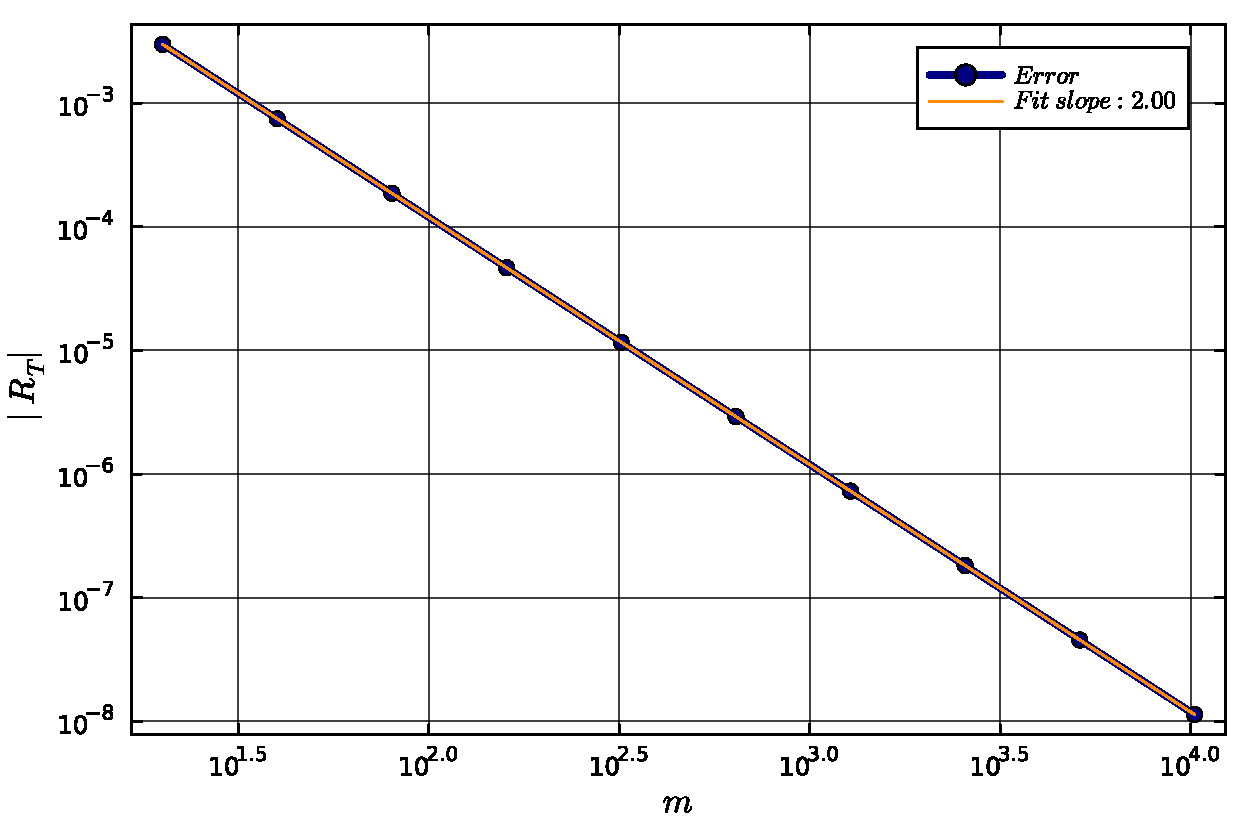
\includegraphics[width=\textwidth]{5123.pdf}
    \end{minipage}
    \hspace{0.5cm}
    \begin{minipage}[b]{0.47\textwidth}
        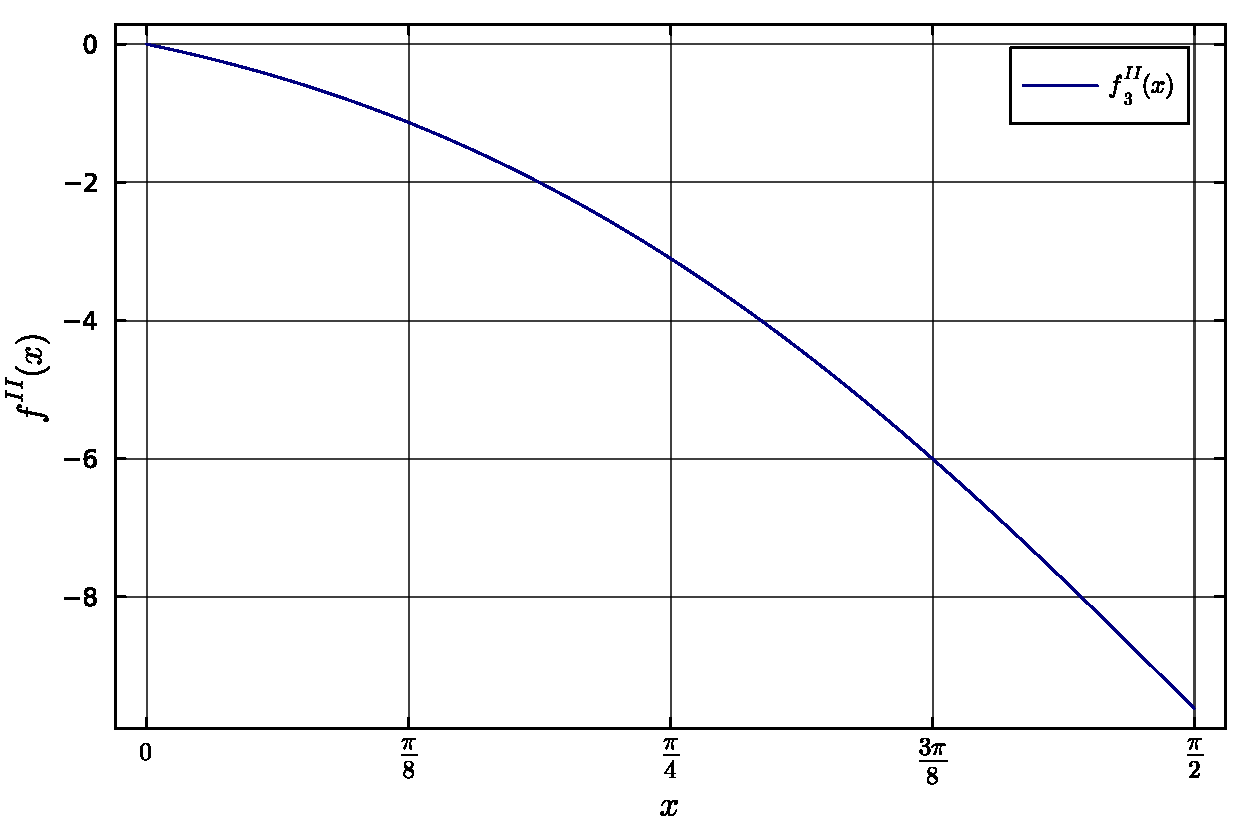
\includegraphics[width=\textwidth]{5123_2.pdf}
    \end{minipage}
    \caption{Studio della regola del trapezio per l'integrale $\int_0^{\pi/2}e^x \cos x\, dx$.}
    \label{fig:es5_1_2_3}
\end{figure}
\begin{figure}[!ht]
    \centering
    \begin{minipage}[b]{0.47\textwidth}
        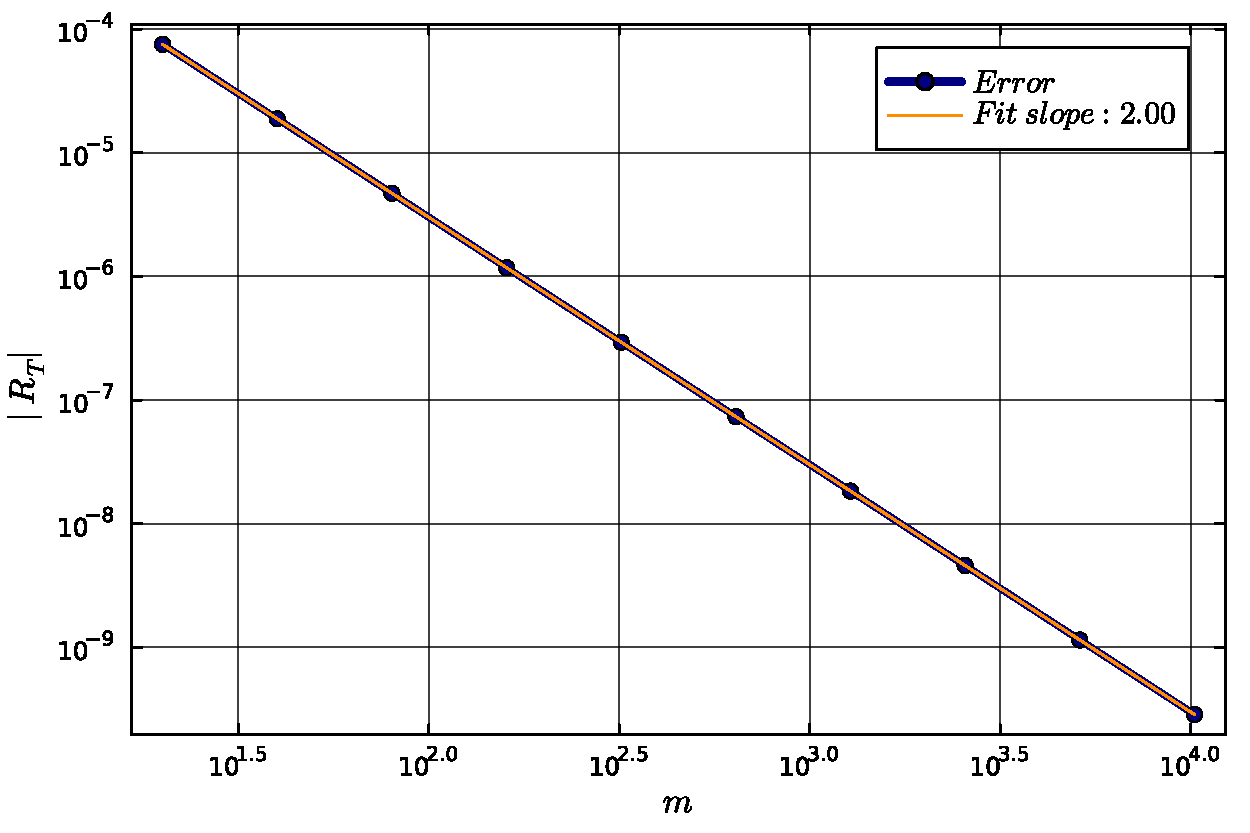
\includegraphics[width=\textwidth]{5124.pdf}
    \end{minipage}
    \hspace{0.5cm}
    \begin{minipage}[b]{0.47\textwidth}
        \includegraphics[width=\textwidth]{5124_2.pdf}
    \end{minipage}
    \caption{Studio della regola del trapezio per l'integrale $\int_0^1 \frac{\tan^{-1}(\sqrt{2+x^2})}{(1+x^2)\sqrt{2+x^2}}\,dx$.}
    \label{fig:es5_1_2_4}
\end{figure}
\begin{figure}[!ht]
    \centering
    \begin{minipage}[b]{0.47\textwidth}
        \includegraphics[width=\textwidth]{5125.pdf}
    \end{minipage}
    \hspace{0.5cm}
    \begin{minipage}[b]{0.47\textwidth}
        \includegraphics[width=\textwidth]{5125_2.pdf}
    \end{minipage}
    \caption{Studio della regola del trapezio per l'integrale $\int_0^1 \sqrt{x} \log(x) \, dx$.}
    \label{fig:es5_1_2_5}
\end{figure}
\begin{figure}[!ht]
    \centering
    \begin{minipage}[b]{0.47\textwidth}
        \includegraphics[width=\textwidth]{5126.pdf}
    \end{minipage}
    \hspace{0.5cm}
    \begin{minipage}[b]{0.47\textwidth}
        \includegraphics[width=\textwidth]{5126_2.pdf}
    \end{minipage}
    \caption{Studio della regola del trapezio per l'integrale $\int_0^1 \sqrt{1-x^2}\, dx$.}
    \label{fig:es5_1_2_6}
\end{figure}

Nei grafici viene riportata la pendenza dell'interpolante dell'errore e nei primi quattro casi l'errore 
decresce con un andamento quadratico nel passo $h$, come atteso. Nel quinto e sesto caso l'errore decresce 
con un ordine inferiore. Come già accennato, questo è dovuto al fatto che l'integranda ha derivata seconda 
non ben definita nel dominio di integrazione.

\paragraph{Commento: } Qui e nei prossimi esercizi l'interpolazione è stata eseguita per l'errore $R_T$ (o $R_S$)
in funzione del passo $h$, e non in funzione del numero di nodi $m$, per mostrare l'andamento quadratico 
(o quartico) dell'errore. I grafici sono stati realizzati in funzione del numero di nodi come richiesto
e quindi la retta di regressione è stata calcolata in funzione del numero di nodi $m$ e non del passo $h$.
Si ricorda che il passo $h$ è legato al numero di nodi $m$ dalle relazioni:
\begin{equation}
    h = \frac{b-a}{m}, \qquad h = \frac{b-a}{2m},
\end{equation}
la prima per la regola del trapezio e la seconda per la regola di Simpson.

\subsection{Esercizi 5.1.3, 5.1.4}
3. Scrivi un programma che implementi la regola di Simpson composta per un intervallo generico $[a,b]$. \\
4. Per ciascun integrale dell'Esercizio 1 sopra, applica la formula di Simpson e confronta gli errori con 
la convergenza di ordine quattro.

\subsubsection{Soluzione}
\paragraph{(3) } Si è implementata la regola di Simpson composta per un intervallo generico $[a,b]$,
e la si è testata nell'esercizio 5.1.4. \\
\paragraph{(4) } Si è calcolato l'integrale con la regola di Simpson per tutti i casi, al variare del numero di
nodi. Oltre alla rappresentazione grafica dell'errore, si sono rappresentate le derivate quarte dell'integranda,
in modo da poter verificare la convergenza di ordine quarto della regola di Simpson. La motivazione
di tale scelta è che l'errore della regola di Simpson scala al quarto ordine con il passo di campionamento,
ma ha per coefficiente la derivata quarta dell'integranda, calcolata in un certo $\xi$ appartenente all'intervallo
in considerazione. In formule:
\[
R_S(h) = -\frac{(b-a)}{180}h^4 f^{(4)}(\xi)
\]
Si riportano nelle figure \ref{fig:es5_1_4_1}, \ref{fig:es5_1_4_2}, \ref{fig:es5_1_4_3},
\ref{fig:es5_1_4_4}, \ref{fig:es5_1_4_5}, \ref{fig:es5_1_4_6} gli studi dei vari casi.
\begin{figure}[!ht]
    \centering
    \begin{minipage}[b]{0.47\textwidth}
        \includegraphics[width=\textwidth]{5141.pdf}
    \end{minipage}
    \hspace{0.5cm}
    \begin{minipage}[b]{0.47\textwidth}
        \includegraphics[width=\textwidth]{5141_2.pdf}
    \end{minipage}
    \caption{Studio della regola di Simpson per l'integrale $\int_0^1 x\log(1+x)\, dx$.}
    \label{fig:es5_1_4_1}
\end{figure}
\begin{figure}[!ht]
    \centering
    \begin{minipage}[b]{0.47\textwidth}
        \includegraphics[width=\textwidth]{5142.pdf}
    \end{minipage}
    \hspace{0.5cm}
    \begin{minipage}[b]{0.47\textwidth}
        \includegraphics[width=\textwidth]{5142_2.pdf}
    \end{minipage}
    \caption{Studio della regola di Simpson per l'integrale $\int_0^1 x^2 \tan^{-1}x\, dx$.}
    \label{fig:es5_1_4_2}
\end{figure}
\begin{figure}[!ht]
    \centering
    \begin{minipage}[b]{0.47\textwidth}
        \includegraphics[width=\textwidth]{5143.pdf}
    \end{minipage}
    \hspace{0.5cm}
    \begin{minipage}[b]{0.47\textwidth}
        \includegraphics[width=\textwidth]{5143_2.pdf}
    \end{minipage}
    \caption{Studio della regola di Simpson per l'integrale $\int_0^{\pi/2}e^x \cos x\, dx$.}
    \label{fig:es5_1_4_3}
\end{figure}
\begin{figure}[!ht]
    \centering
    \begin{minipage}[b]{0.47\textwidth}
        \includegraphics[width=\textwidth]{5144.pdf}
    \end{minipage}
    \hspace{0.5cm}
    \begin{minipage}[b]{0.47\textwidth}
        \includegraphics[width=\textwidth]{5144_2.pdf}
    \end{minipage}
    \caption{Studio della regola di Simpson per l'integrale $\int_0^1 \frac{\tan^{-1}(\sqrt{2+x^2})}{(1+x^2)\sqrt{2+x^2}}\,dx$.}
    \label{fig:es5_1_4_4}
\end{figure}
\begin{figure}[!ht]
    \centering
    \begin{minipage}[b]{0.47\textwidth}
        \includegraphics[width=\textwidth]{5145.pdf}
    \end{minipage}
    \hspace{0.5cm}
    \begin{minipage}[b]{0.47\textwidth}
        \includegraphics[width=\textwidth]{5145_2.pdf}
    \end{minipage}
    \caption{Studio della regola di Simpson per l'integrale $\int_0^1 \sqrt{x} \log(x) \, dx$.}
    \label{fig:es5_1_4_5}
\end{figure}
\begin{figure}[!ht]
    \centering
    \begin{minipage}[b]{0.47\textwidth}
        \includegraphics[width=\textwidth]{5146.pdf}
    \end{minipage}
    \hspace{0.5cm}
    \begin{minipage}[b]{0.47\textwidth}
        \includegraphics[width=\textwidth]{5146_2.pdf}
    \end{minipage}
    \caption{Studio della regola di Simpson per l'integrale $\int_0^1 \sqrt{1-x^2}\, dx$.}
    \label{fig:es5_1_4_6}
\end{figure}

Si può osservare che l'errore decresce con un andamento quartico nei primi quattro casi, come atteso, ma non negli
ultimi due casi, in cui la derivata quarta è non ben definita. In questi casi l'errore decresce con un ordine 
inferiore. Nei casi in cui l'errore decresce con un ordine quartico, si osserva che l'errore scende rapidamente
fino a valore di $\epsilon_{mach}$, per poi stabilizzarsi per motivazioni numeriche. Chiaramente l'interpolazione
dell'errore è stata eseguita solo sui punti che si trovano al di sopra di questo valore.

\subsection{Esercizio 5.3.1}
1. Scrivi un programma che calcoli i nodi e i pesi per la quadratura di Gauss-Legendre nell’intervallo $[-1,1]$. 
Di seguito alcuni suggerimenti per l'implementazione. \\
(a) Per trovare le radici $x_k$, con $k=1,\ldots,n$, del polinomio di Legendre $P_n(x)$ di ordine $n$, 
usa il metodo di Newton. Come condizione iniziale per la $k$-esima radice, utilizza

\begin{equation}
    x^{(0)}_k=\cos(\phi_k)\,,
    \qquad
    \phi_k= \frac{4k-1}{4n+2}\pi\,.
\end{equation}
    
(b) Per applicare il metodo di Newton è necessario valutare $P_n(x_k^{(i)})$ e la derivata $P'_n(x_k^{(i)})$, 
dove $x_k^{(i)}$ è la $i$-esima iterazione nella ricerca della $k$-esima radice $x_k$. 
Puoi ottenerle risolvendo la relazione di ricorrenza

\begin{equation}
    (m+1)P_{m+1}(x) = (2m+1)xP_{m}(x) - mP_{m-1}(x)\,,
\end{equation}

per $m=1,\ldots,n-1$, dove $P_0(x) = 1$ e $P_1(x) = x$, con $x=x^{(i)}_k$. La derivata si calcola poi tramite 
la relazione

\begin{equation}
    (x^{2}-1)P'_{n}(x)=n[xP_{n}(x)-P_{n-1}(x)]\,. 
\end{equation}

(c) Una volta raggiunta la radice $x_k$ entro una certa tolleranza, il valore della derivata $P'_n(x_k)$ 
permette di ottenere il peso corrispondente tramite:

\begin{equation}
    \label{eq:gauss_legendre_weight}
    w_k= \frac{2}{(1-x_k^2)[P'_n(x_k)]^2}\,.
\end{equation}

(d) Verifica i tuoi risultati confrontandoli con quelli tabulati.

\subsubsection{Soluzione}
Per comodità di implementazione la soluzione riporta i quattro passaggi nel seguente ordine: (b), (a), (c), (d).
\paragraph{(b) } Si è sviluppato un algoritmo che calcola sia i polinomi di Legendre $P_n(x)$ che le loro derivate $P'_n(x)$
utilizzando la relazione di ricorrenza indicata nell'esercizio. Si riporta in figura \ref{fig:es5_3_1_1} il grafico 
dei polinomi e delle loro derivate fino ad ordine $n = 4$.
\begin{figure}[!ht]
    \centering
    \includegraphics[width=0.8\textwidth]{5311.pdf}
    \caption{Polinomi di Legendre $P_n(x)$ e le loro derivate $P'_n(x)$ fino ad ordine $n=4$.}
    \label{fig:es5_3_1_1}
\end{figure}
\paragraph{(a) (b) } Si è implementato il metodo di Newton per trovare le radici dei polinomi di Legendre $P_n(x)$ 
e dei pesi associati. Una volta calcolati gli zeri di $P_n(x)$, si sono trovati i pesi associati utilizzando 
la formula \ref{eq:gauss_legendre_weight}.
Si riporta in tabella \ref{tab:legendre_ordine4} il confronto tra i nodi e pesi calcolati con i 
corrispettivi valori tabulati, con ordine del polinomio $n = 4$. 

\begin{table}[ht]
\centering
\caption{Confronto tra zeri e pesi del polinomio di Legendre di ordine 4}
\label{tab:legendre_ordine4}
\begin{tabular}{|c|c!{\vrule width 1.2pt}c|c|}
\hline
\( x_i \) & \( x_i^{\text{tab}} \) & \( w_i \) & \( w_i^{\text{tab}} \) \\
\hline
 0.86114  &  0.86114 & 0.65215 & 0.65215 \\
 0.33998  &  0.33998 & 0.34785 & 0.34785 \\
-0.33998  & -0.33998 & 0.34785 & 0.34785 \\
-0.86114  & -0.86114 & 0.65215 & 0.65215 \\
\hline
\end{tabular}
\end{table}

\subsection{Esercizio 5.4.1}
Per ciascun integrale, calcola le approssimazioni utilizzando le regole di quadratura di Gauss-Legendre e 
Clenshaw-Curtis con $n=4,6,8,\ldots,40$. Rappresenta graficamente gli errori $|I_n-I|$ di entrambi i metodi 
in funzione di $n$ su una scala semi-logaritmica. (Suggerimento: considera di implementare la regola di 
Clenshaw-Curtis solo per $n$ pari.)

\begin{itemize}
    \item[(a)] $\displaystyle\int_{-1}^1 e^{-4x}\, dx = \frac{1}{2}\sinh(4)$
    \item[(b)] $\displaystyle\int_{-1}^1 e^{-9x^2}\, dx = \frac{\sqrt{\pi}}{3}\, \operatorname{erf}(3)$
    \item[(c)] $\displaystyle\int_{-1}^1 \operatorname{sech}(x) \, dx = 2 \tan^{-1} [ \sinh (1) ]$
    \item[(d)] $\displaystyle\int_{-1}^1 \frac{1}{1+9x^2}\, dx = \frac{2}{3} \tan^{-1}(3)$
    \item[(e)] $\displaystyle\int_{\pi/2}^{\pi} x^2 \sin 8x \, d x = -\frac{3 \pi^2}{32}$
\end{itemize}

\subsubsection{Soluzione}
Per ciascun integrale, sono state calcolate le approssimazioni utilizzando le regole di quadratura di 
Gauss-Legendre e Clenshaw-Curtis con $n=4,6,8,\ldots,40$. Gli errori $|I_n-I|$ di entrambi i metodi 
sono stati rappresentati graficamente in funzione di $n$ su una scala semi-logaritmica.\\
I grafici saranno presentati non nell'ordine in cui sono stati richiesti, ma dapprima gli integrali di
funzioni olomorfe, poi quelli di funzioni non olomorfe. \\
Si riportano in figura \ref{fig:es5_4_1_1}, gli studi degli errori per gli integrali di funzioni olomorfe.

\begin{figure}[!ht]
    \centering
    \begin{minipage}[b]{0.47\textwidth}
        \includegraphics[width=\textwidth]{5411.pdf}
        \caption*{(a)}
    \end{minipage}
    \hspace{0.5cm}
    \begin{minipage}[b]{0.47\textwidth}
        \includegraphics[width=\textwidth]{5412.pdf}
        \caption*{(b)}
    \end{minipage}
    \begin{minipage}[b]{0.47\textwidth}
        \includegraphics[width=\textwidth]{5415.pdf}
        \caption*{(e)}
    \end{minipage}
    \caption{Studio degli errori per gli integrali di funzioni olomorfe.}
    \label{fig:es5_4_1_1}
\end{figure}

I grafici di figura \ref{fig:es5_4_1_1} mostrano che gli errori decrescono in maniera molto rapida all'aumentare
di $n$, raggiungendo l'ordine di grandezza di $\epsilon_{mach}$ per $n$ piccoli. Questo fenomeno è legato 
alla regolarità dell'integranda, che è olomorfa in tutto l'intervallo di integrazione. \\
Un'altro comportamento degno di nota è che gli errori del metodo di Clenshaw-Curtis sono più grandi di quelli
del metodo di Gauss-Legendre, questo è legato al fatto che il metodo di Clenshaw-Curtis integra esattamente 
polinomi di grado $n-1$ mentre il metodo di Gauss-Legendre integra esattamente polinomi di grado $2n-1$. \\
Infine si può mostrare matematicamente che inizialmente gli errori del metodo di Clenshaw-Curtis coincidono
con gli errori del metodo di Gauss-Legendre. \\
Si riportano in figura \ref{fig:es5_4_1_2}, gli studi degli errori per gli integrali di funzioni non olomorfe.
\begin{figure}[!ht]
    \centering
    \begin{minipage}[b]{0.47\textwidth}
        \includegraphics[width=\textwidth]{5413.pdf}
        \caption*{(c)}
    \end{minipage}
    \hspace{0.5cm}
    \begin{minipage}[b]{0.47\textwidth}
        \includegraphics[width=\textwidth]{5414.pdf}
        \caption*{(d)}
    \end{minipage}
    \caption{Studio degli errori per gli integrali di funzioni non olomorfe.}
    \label{fig:es5_4_1_2}
\end{figure}

Nei casi di figura \ref{fig:es5_4_1_2} si è potuto studiare l'errore in maniera più accurata tramite le ellissi
di Bernstein. Dalla teoria è noto che la più grande ellissi nel piano complesso che non contiene singolarità e 
definita da: 
\begin{equation}
    E_\rho = \left\{ z \in C : z = \frac{1}{2} \left( \rho e^{i\theta} + \rho^{-1} e^{-i\theta} \right), \; \theta \in [0, 2\pi) \right\}\,.
\end{equation}

determina il parametro $\rho$ delle seguenti maggiorazioni:

\begin{equation}
    \label{eq:errors_CC_GL}
    |I[f]-I_n[f]| \leq \frac{64}{15} \frac{M\rho^{1-n}}{\rho^2-1}\,, \qquad |I[f]-I_n[f]| \leq \frac{64}{15} \frac{M\rho^{-2n}}{\rho^2-1}\,.
    \end{equation}

dove la prima riguarda Clenshaw-Curtis, la seconda Gauss-Legendre.\\
Si è perciò calcolato il parametro $\rho$ in entrambi i casi, sapendo che le singolarità delle integrande estese
al piano complesso si trovano in $\frac{i \pi}{2} + ik\pi$ per $k \in N$ nel primo caso, in $\pm i\frac{1}{3}$
nel secondo. Tramite $\rho$ si sono stimati i limiti superiori degli errori al variare di $n$. Nei grafici 
vengono riportate le rette, ma dato che in \ref{eq:errors_CC_GL} è presente anche la maggiorazione con $M$, 
il grafico si concentra sulla pendenza e non sulla traslazione verticale. Si può notare che nel caso (c) 
le rette ricalcano precisamente la pendenza degli errori. Nel caso (d) l'andamento di Curtis è rispettato, mentre 
Legendre necessita di più punti per poter entrare nel regime in cui l'errore scala come $O(n^2)$. D'altra parte, 
l'accuratezza massima raggiunta nel caso del metodo (d) è dell'ordine di $10^{-11}$, molto più alta rispetto
agli altri casi. Infine, per i valori di $n$ considerati, i due metodi non escono dalla regione in cui gli
errori sono gli stessi. Per queste ragioni nel caso (d) la pendenza della retta nel caso di Gauss-Legendre
non coincide con quella degli errori. \\

\subsection{Esercizio 5.4.2}
Per ciascun integrale improprio, calcola le approssimazioni utilizzando la regola di quadratura double-exponential 
appropriata con $N=n/2$ e $n=4,6,8,\ldots,60$. Rappresenta graficamente gli errori in funzione di $n$ 
su una scala semi-logaritmica.

\begin{itemize}
    \item[(a)] $\displaystyle\int_{-\infty}^\infty \frac{1}{1+x^2+x^4}\, dx = \frac{\pi}{\sqrt{3}}$
    \item[(b)] $\displaystyle\int_{-\infty}^\infty e^{-x^2}\cos(x)\, dx = e^{-1/4}\sqrt{\pi}$
    \item[(c)] $\displaystyle\int_{-\infty}^\infty (1+x^2)^{-2/3}\, dx = \frac{\sqrt{\pi}\,\Gamma(1/6)}{\Gamma(2/3)}$
    \item[(d)] $\displaystyle \int_{0}^{\infty} \frac{1}{1+x^2}\,dx = \frac{\pi}{2}$
    \item[(e)] $\displaystyle \int_0^\infty \frac{e^{-x}}{\sqrt{x}}\,dx = \sqrt{\pi}$
\end{itemize}

\subsubsection{Soluzione}
Si riportano nelle figure \ref{fig:es5_4_2_1} e \ref{fig:es5_4_2_2} gli studi degli errori per gli integrali 
impropri, con la regola di quadratura double-exponential.
\begin{figure}[!ht]
    \centering
    \begin{minipage}[b]{0.47\textwidth}
        \includegraphics[width=\textwidth]{5421.pdf}
        \caption*{(a)}
    \end{minipage}
    \hspace{0.5cm}
    \begin{minipage}[b]{0.47\textwidth}
        \includegraphics[width=\textwidth]{5422.pdf}
        \caption*{(b)}
    \end{minipage}
    \begin{minipage}[b]{0.47\textwidth}
        \includegraphics[width=\textwidth]{5423.pdf}
        \caption*{(c)}
    \end{minipage}
    \begin{minipage}[b]{0.47\textwidth}
        \includegraphics[width=\textwidth]{5424.pdf}
        \caption*{(d)}
    \end{minipage}
    \caption{Studio degli errori per gli integrali impropri con la regola di quadratura double-exponential.}
    \label{fig:es5_4_2_1}
\end{figure}
In figura \ref{fig:es5_4_1_2} possiamo notare che gli integrali convergono nonostante la presenza di singolarità
nelle integrande, questo è uno dei vantaggi della regola di quadratura double-exponential. 
\begin{figure}[!ht]
    \centering
    \begin{minipage}[b]{0.47\textwidth}
        \includegraphics[width=\textwidth]{5425.pdf}
        \caption*{(e)}
    \end{minipage}
    \caption{Studio degli errori per l'integrale improprio con la regola di quadratura double-exponential.}
    \label{fig:es5_4_2_2}
\end{figure}

Nella figura \ref{fig:es5_4_2_2} si sono rappresentati gli errori dell'integrazione secondo la regola di quadratura
double-exponential, ma in un caso con l'utilizzo del cambio di variabile apposito per funzioni con $e^-x$, 
nell'altro senza. Si può notare che nel primo caso l'errore ha una convergenza molto più rapida, raggiungendo 
l'ordine di $\epsilon_{mach}$.

\subsection{Esercizio 5.4.3}
Per ciascun integrale, calcola le approssimazioni utilizzando la regola di quadratura di Gauss-Legendre 
con $n=4,6,8,\ldots,60$ e la regola di quadratura double-exponential appropriata con $N=n/2$. 
Rappresenta graficamente gli errori in funzione di $n$ su una scala semi-logaritmica.

\begin{itemize}
    \item[(a)] $\displaystyle \int_0^1 \sqrt{x} \log(x) \, dx = -\frac{4}{9}$
    \item[(b)] $\displaystyle \int_0^1 \sqrt{1-x^2}\, dx = \frac{\pi}{4}$
    \item[(c)] $\displaystyle \int_0^1 (\log x)^2\, dx = 2$
    \item[(d)] $\displaystyle \int_0^{\pi/2} \log(\cos(x))\, dx = -\frac{\pi}{2}\log(2)$
    \item[(e)] $\displaystyle \int_0^{\pi/2} \sqrt{\tan(x)}\, dx = \dfrac{\pi}{\sqrt{2}}$
\end{itemize}

\subsubsection{Soluzione}
Si riportano in figura \ref{fig:es5_4_3_1} gli studi degli errori per gli integrali con la regola di quadratura 
di Gauss-Legendre, insieme agli errori della regola di quadratura double-exponential.
\begin{figure}[!ht]
    \centering
    \begin{minipage}[b]{0.47\textwidth}
        \includegraphics[width=\textwidth]{5431.pdf}
        \caption*{(a)}
    \end{minipage}
    \hspace{0.5cm}
    \begin{minipage}[b]{0.47\textwidth}
        \includegraphics[width=\textwidth]{5432.pdf}
        \caption*{(b)}
    \end{minipage}
    \begin{minipage}[b]{0.47\textwidth}
        \includegraphics[width=\textwidth]{5433.pdf}
        \caption*{(c)}
    \end{minipage}
    \begin{minipage}[b]{0.47\textwidth}
        \includegraphics[width=\textwidth]{5434.pdf}
        \caption*{(d)}
    \end{minipage}
    \begin{minipage}[b]{0.47\textwidth}
        \includegraphics[width=\textwidth]{5435.pdf}
        \caption*{(e)}
    \end{minipage}
    \caption{Studio degli errori per gli integrali con la regola di quadratura di Gauss-Legendre e double-exponential.}
    \label{fig:es5_4_3_1}
\end{figure}

RIVEDI QUESTE CONSIDERAZIONI: \\
Dai grafici risulta evidente che gli errori della regola di quadratura di Gauss-Legendre decrescono molto
più rapidamente rispetto a quelli della regola di quadratura double-exponential. Con questo esercizio, unitamente
agli esercizi 5.4.1 e 5.4.2, giungiamo alla conclusione che la regola di Gauss-Legendre è l'algoritmo più
rapido per il calcolo di integrali di funzioni regolari, almeno per la nostra implementazione. 
Lo svantaggio è che non riesce a integrare tutte le funzioni, per cui bisogna ricorrere alla quadratura 
double-exponential nel caso di funzioni con singolarità, nonostante sia molto più lento. In generale però
si può considerare l'algoritmo di Clenshaw-Curtis con l'uso della "fast Fourier transform" (FFT), aumentandone
l'efficienza.

\section{Equazioni differenziali ordinarie}
\subsection{Esercizi 6.2.1, 6.2.2}
1. Scrivi un programma che implementi il metodo di Eulero per risolvere un \textit{sistema} 
di equazioni differenziali.\\
2. Per ciascun problema ai valori iniziali (IVP), risolvi il problema usando il metodo di Eulero. \\
(i) Traccia il grafico della soluzione per $n=320$. \\
(ii) Per $n=10\cdot2^k$, $k=2,3,\ldots,10$, calcola l'errore come 
$||u-\hat{u}||_\infty=\max_{0\leq i\leq n} |u_i-\hat{u}(t_i)|$ e all'istante finale, $|u_n-\hat{u}(t_n)|$. 
Realizza un grafico di convergenza log-log, includendo una retta di riferimento per la convergenza del 
primo ordine.\\
(a) $u' = -2t u$, $\ 0 \le t \le 2$, $\ u(0) = 2$;  
$\quad$ $\hat{u}(t) = 2e^{-t^2}$ \\
(b) $u' = u + t$, $\ 0 \le t \le 1$, $\ u(0) = 2$;  
$\quad$ $\hat{u}(t) = -1-t+3e^t$ \\
(c) $(1+t^3)uu' = t^2$, $\ 0 \le t \le 3$, $\ u(0) =1$; 
$\quad$ $\hat{u}(t) = [1+(2/3)\ln (1+t^3)]^{1/2}$

\subsubsection{Soluzione}
Si è implementato il metodo di Eulero per risolvere un sistema di equazioni differenziali. La funzione che 
sviluppa il metodo viene testata nei prossimi esercizi, sia nel caso di equazioni che di sistemi di equazioni.\\
Si riportano nelle figure \ref{fig:es6_2_1_1}, \ref{fig:es6_2_1_2}, \ref{fig:es6_2_1_3} i grafici delle soluzioni, 
uniti ai grafici degli errori per i tre casi richiesti. Le soluzioni sono calcolate per $n = 320$ come richiesto,
i grafici degli errori corrispondono a più soluzioni con $n$ che varia da $10\cdot2^k$ con $k=2,3,\ldots,10$.
\begin{figure}[!ht]
    \centering
    \begin{minipage}[b]{0.47\textwidth}
        \includegraphics[width=\textwidth]{6221.pdf}
    \end{minipage}
    \hspace{0.5cm}
    \begin{minipage}[b]{0.47\textwidth}
        \includegraphics[width=\textwidth]{6222.pdf}
    \end{minipage}
    \caption{Soluzione e errore per il caso (a).}
    \label{fig:es6_2_1_1}
\end{figure}
\begin{figure}[!ht]
    \centering
    \begin{minipage}[b]{0.47\textwidth}
        \includegraphics[width=\textwidth]{6223.pdf}
    \end{minipage}
    \hspace{0.5cm}
    \begin{minipage}[b]{0.47\textwidth}
        \includegraphics[width=\textwidth]{6224.pdf}
    \end{minipage}
    \caption{Soluzione e errore per il caso (b).}
    \label{fig:es6_2_1_2}
\end{figure}
\begin{figure}[!ht]
    \centering
    \begin{minipage}[b]{0.47\textwidth}
        \includegraphics[width=\textwidth]{6225.pdf}
    \end{minipage}
    \hspace{0.5cm}
    \begin{minipage}[b]{0.47\textwidth}
        \includegraphics[width=\textwidth]{6226.pdf}
    \end{minipage}
    \caption{Soluzione e errore per il caso (c).}
    \label{fig:es6_2_1_3}
\end{figure}

La prima osservazione che si può fare riguarda la convergenza del metodo di Eulero. In tutti i grafici
gli errori sono stati calcolati sia come $||u-\hat{u}||_\infty=\max_{0\leq i\leq n} |u_i-\hat{u}(t_i)|$ che come
$|u_n-\hat{u}(t_n)|$. In entrambi i casi si osserva che gli errori decrescono con un ordine di grandezza
prossimo a $O(h)$, come atteso per il metodo di Eulero. Nei grafici infatti è stato riportato il coefficiente
angolare dell'interpolazione degli errori con il metodo dei minimi quadrati. In tutti e tre i casi, per ciascuna
tipologia di errore, il coefficiente angolare è prossimo a $-1$. \\
La seconda osservazione riguarda la differenza tra i due tipi di errore. Si osserva che solo nel primo grafico 
le due rette degli errori sono distinte, mentre negli altri due casi sono sovrapposte. Questo è lo stesso 
comportamento che si è studiato nella teoria, in cui perturbazioni del valore iniziale influenzano la soluzione.
L'esempio fatto riguardava le due equazioni differenziali lineari $u' = u$ e $u' = -u $, in cui la soluzione
della prima equazione amplifica gli errori, mentre la soluzione della seconda equazione li smorza. 
Nel nostro caso, la soluzione dell'equazione (a) smorza gli errori avanzando nel tempo, per cui il massimo 
errore non si raggiunge all'istante finale. La diretta conseguenza è che le rette sono distinte.
Negli altri due casi invece la soluzione amplifica gli errori, portando a rette sovrapposte.

\subsection{Esercizio 6.2.3}
Risolvi i seguenti problemi ai valori iniziali (IVP) con il metodo di Eulero utilizzando $n=1000$ passi. 
Traccia in un unico grafico la soluzione e la sua derivata prima, e in un altro grafico rappresenta l'errore 
in ciascuna componente in funzione del tempo.\\
\begin{enumerate}[label=(\alph*)]
    \item $y''+ 9y = \sin(2t)$, \quad $0< t< 2\pi$, \quad $y(0) = 2$, \ $y'(0) = 1$;\\[2pt]
    \hspace*{1.5em} $\hat{y}(t) = \dfrac{1}{5} \sin(3t) + 2 \cos (3t) + \dfrac{1}{5} \sin (2t)$
    \item $y''- 4y = 4t$, \quad $0< t< 1.5$, \quad $y(0) = 2$, \ $y'(0) = -1$;\\[2pt]
    \hspace*{1.5em} $\hat{y}(t) = e^{2t} + e^{-2t} - t$
    \item $y''+ 4y'+ 4y = t$, \quad $0< t< 4$, \quad $y(0) = 1$, \ $y'(0) = \dfrac{3}{4}$;\\[2pt]
    \hspace*{1.5em} $\hat{y}(t) = (3t+\frac{5}{4})e^{-2t} + \frac{t-1}{4}$
\end{enumerate}

\subsubsection{Soluzione}
Fissato $n = 1000$ si è risolto il problema ai valori iniziali (IVP) con il metodo di Eulero. Per prima cosa
si sono riscritte le equazioni differenziali di secondo ordine come un sistema di equazioni differenziali
di primo ordine, in modo da poter utilizzare il metodo di Eulero:
\begin{align*}
\left\{
\begin{array}{rl}
    z_1' &= z_2 \\
    z_2' &= -9z_1 + \sin(2t) \\
    z_1(0) &= 2 \\
    z_2(0) &= 1
\end{array}
\right.
\qquad
\left\{
\begin{array}{rl}
    z_1' &= z_2 \\
    z_2' &= 4z_1 + 4t \\
    z_1(0) &= 2 \\
    z_2(0) &= -1
\end{array}
\right.
\qquad
\left\{
\begin{array}{rl}
    z_1' &= z_2 \\
    z_2' &= -4z_1 - 4z_2 + t \\
    z_1(0) &= 1 \\
    z_2(0) &= \dfrac{3}{4}
\end{array}
\right.
\end{align*}

Scritte così si è potuto utilizzare il metodo di Eulero per sistemi di equazioni differenziali.
Si riportano in figura \ref{fig:es6_2_3_1}, \ref{fig:es6_2_3_2}, \ref{fig:es6_2_3_3} i grafici delle soluzioni
e delle loro derivate prime, insieme ai grafici degli errori per i tre casi richiesti. Gli errori rappresentano 
la distanza tra la soluzione calcolata e quella esatta, in ciascuna componente del sistema.
\begin{figure}[!ht]
    \centering
    \begin{minipage}[b]{0.47\textwidth}
        \includegraphics[width=\textwidth]{6231.pdf}
    \end{minipage}
    \hspace{0.5cm}
    \begin{minipage}[b]{0.47\textwidth}
        \includegraphics[width=\textwidth]{6232.pdf}
    \end{minipage}
    \caption{Soluzione e derivata prima per il caso (a). Errori.}
    \label{fig:es6_2_3_1}
\end{figure}
\begin{figure}[!ht]
    \centering
    \begin{minipage}[b]{0.47\textwidth}
        \includegraphics[width=\textwidth]{6233.pdf}
    \end{minipage}
    \hspace{0.5cm}
    \begin{minipage}[b]{0.47\textwidth}
        \includegraphics[width=\textwidth]{6234.pdf}
    \end{minipage}
    \caption{Soluzione e derivata prima per il caso (b). Errori.}
    \label{fig:es6_2_3_2}
\end{figure}
\begin{figure}[!ht]
    \centering
    \begin{minipage}[b]{0.47\textwidth}
        \includegraphics[width=\textwidth]{6235.pdf}
    \end{minipage}
    \hspace{0.5cm}
    \begin{minipage}[b]{0.47\textwidth}
        \includegraphics[width=\textwidth]{6236.pdf}
    \end{minipage}
    \caption{Soluzione e derivata prima per il caso (c). Errori.}
    \label{fig:es6_2_3_3}
\end{figure}

Nelle figure \ref{fig:es6_2_3_1} e \ref{fig:es6_2_3_2} è possibile notare che gli errori aumentano insieme al 
tempo. Infatti nel caso (a) la soluzione esatta è una combinazione di funzioni trigonometriche, per cui 
le perturbazioni iniziali si amplificano nel tempo. Nel caso (b) si ha lo stesso comportamento perchè a tempi 
più grandi domina l'esponenziale $e^{2t}$, che amplifica le perturbazioni iniziali. \\
Al contrario in figura \ref{fig:es6_2_3_3} si osserva che gli errori decrescono nel tempo, questo perchè la 
soluzione esatta è esponenziale decrescente, e così smorza l'errore.

\subsection{Esercizio 6.3.1}
(a) Scrivi un programma che risolva un sistema di equazioni differenziali utilizzando il metodo IE2 
(Eulero implicito esplicito di ordine 2).\\
(b) Scrivi un programma che risolva un sistema di equazioni differenziali utilizzando il metodo RK4 
(Runge-Kutta del quarto ordine).\\
(c) Testa la tua implementazione dei metodi IE2 e RK4 sul problema ai valori iniziali\\

$u' = -2t u$, $\ 0 \le t \le 2$, $\ u(0) = 2$; \\
$\hat{u}(t) = 2e^{-t^2}$ \\

Risolvi per $n=30,60,90,\ldots,300$ e rappresenta graficamente l'errore massimo 
$||u-\hat{u}||_\infty=\max_{0\leq i\leq n} |u_i-\hat{u}(t_i)|$ in funzione del numero di valutazioni 
di funzione in un grafico log-log, insieme a una retta che mostri il tasso di convergenza atteso.

\subsubsection{Soluzione}
Si sono implementati i due metodi richiesti e applicati al problema ai valori iniziali (IVP) presentato.
In figura \ref{fig:es6_3_1} si riportano i grafici degli errori per i due metodi,
calcolati per $n=30,60,90,\ldots,300$.
\begin{figure}[!ht]
    \centering
    \includegraphics[width=0.8\textwidth]{6311.pdf}
    \caption{Confronto tra gli errori dei metodi IE2 e RK4.}
    \label{fig:es6_3_1}
\end{figure}
Nel grafico sono state tracciate le rette interpolanti degli errori, ottenute con il metodo dei minimi quadrati. 
Di tali rette sono riportate sul grafico le pendenze, in accordo con la teoria. Il metodo IE2 infatti deve avere 
un ordine di convergenza pari a $2$, mentre il metodo RK4 deve avere un ordine di convergenza pari a $4$. \\
I grafici sono stati realizzati in funzione del numero di valutazioni della funzione. Sapendo che IE2 richiede $2$
valutazioni della funzione per ogni passo, e che RK4 richiede $4$ valutazioni della funzione per ogni passo,
si può spiegare il fatto che i punti del grafico si trovano incolonnati uno ogni due passi di IE2. \\
Infine si può notare che a parità di numero di valutazioni della funzione, il metodo RK4 ha un errore molto più 
piccolo rispetto al metodo IE2, evidenziandone l'efficacia.

\subsection{Esercizio 6.3.2}
\label{es:6_3_2}
In ciascuno dei seguenti casi, utilizza l'integratore RK4 per risolvere il sistema di ODE per $0\le t \le 10$ 
con le condizioni iniziali indicate. (A tal fine, devi trovare una procedura sensata per scegliere il 
numero di passi $n$ da utilizzare.) Rappresenta i risultati come curve nel piano delle fasi, cioè con $x$ e $y$ 
come assi del grafico.
\begin{align*}
\text{(a)}\quad 
\begin{cases}
x' = -4y + x(1 - x^2 - y^2) \\
y' = 4x + y(1 - x^2 - y^2)
\end{cases}
\quad 
\\
\vspace{2em}
\text{con } [x(0), y(0)] = [0.1, 0],\ [0, 1.9]
\end{align*}
\begin{align*}
\text{(b)}\quad 
\begin{cases}
x' = -4y - \dfrac{1}{4}x(1 - x^2 - y^2)(4 - x^2 - y^2) \\
y' = 4x - \dfrac{1}{4}y(1 - x^2 - y^2)(4 - x^2 - y^2)
\end{cases}
\\
\vspace{2em}
\text{con } [x(0), y(0)] = [0.95, 0],\quad [0, 1.05],\quad [-2.5, 0]
\end{align*}

\subsubsection{Soluzione}
Si sono risolti i due sistemi di equazioni differenziali con il metodo RK4, per ciascuna delle condizioni iniziali
indicate. Al fine di stimare un valore per il passo h, si è scelto di utilizzare il seguente algoritmo:
\begin{enumerate}
    \item Si sceglie un numero di passi iniziale $n$.
    \item Si calcola la soluzione per $n$ passi, ottenendo la soluzione $u$.
    \item Si calcola la soluzione per $2n$ passi, ottenendo la soluzione $\tilde{u}$.
    \item Si calcola l'errore come $||u - \tilde{u}||_\infty$, dove di $\tilde{u}$ si scelgono 
    solo i punti che corrispondono a $u$.
    \item Se l'errore è maggiore di una tolleranza $\epsilon$, si raddoppia il passo e si torna al punto 2,
    altrimenti l'algoritmo si interrompe, restituisce $n$ e $h = \frac{b-a}{n}$.
\end{enumerate}

Per tutte le condizioni iniziali si è scelto come tolleranza $\epsilon = 10^{-6}$, e come numero di punti iniziali
$n = 1000$. \\
Da notare che nell'algoritmo presentato ad ogni passo bisogna calcolare solamente una nuova soluzione perchè si 
riutilizza quella precedente. Con l'algoritmo proposto si riesce a stimare un valore di $h$ che garantisca
un errore inferiore alla tolleranza, ma non è certamente paragonabile al metodo adattivo, che permette 
di scegliere il passo in maniera più efficiente, a ogni passaggio. \\
Si riportano in figura \ref{fig:es6_3_2_1}, \ref{fig:es6_3_2_2} i grafici delle soluzioni ottenute,
rappresentate come curve nel piano delle fasi, per i due casi richiesti. Inoltre si sono rappresentate le 
soluzioni in tre dimensioni, con il tempo come terza coordinata.
\begin{figure}[!ht]
    \centering
    \begin{minipage}[b]{0.47\textwidth}
        \includegraphics[width=\textwidth]{632A1.pdf}
    \end{minipage}
    \hspace{0.5cm}
    \begin{minipage}[b]{0.47\textwidth}
        \includegraphics[width=\textwidth]{632A2.pdf}
    \end{minipage}
    \caption{Soluzioni del sistema di ODE (a).}
    \label{fig:es6_3_2_1}
\end{figure}
\begin{figure}[!ht]
    \centering
    \begin{minipage}[b]{0.47\textwidth}
        \includegraphics[width=\textwidth]{632B1.pdf}
    \end{minipage}
    \hspace{0.5cm}
    \begin{minipage}[b]{0.47\textwidth}
        \includegraphics[width=\textwidth]{632B2.pdf}
    \end{minipage}
    \begin{minipage}[b]{0.47\textwidth}
        \includegraphics[width=\textwidth]{632B3.pdf}
    \end{minipage}
    \caption{Soluzioni del sistema di ODE (b).}
    \label{fig:es6_3_2_2}
\end{figure}

Infine si riportano in tabella \ref{tab:valori_h} i valori di $h$ ottenuti tramite il metodo precedentemente descritto.
\begin{table}[!ht]
    \centering
    \caption{Valori di $h$ ottenuti per i due sistemi di ODE}
    \label{tab:valori_h}
    \begin{tabular}{|l|c|c|}
        \hline
        \textbf{Sistema} & \textbf{Condizioni iniziali} & \textbf{$h$} \\
        \hline
        (a) & $[0.1, 0]$ & 0.0025 \\
        (a) & $[0, 1.9]$ & 0.0025 \\
        (b) & $[0.95, 0]$ & 0.0025 \\
        (b) & $[0, 1.05]$ & 0.00125 \\
        (b) & $[-2.5, 0]$ & 0.00125 \\
        \hline
    \end{tabular}
\end{table}

\subsection{Esercizio 6.3.3}
Una malattia endemica in una popolazione può essere modellata tracciando la frazione di popolazione suscettibile 
all'infezione, $v(t)$, e la frazione infetta, $w(t)$. (Il resto della popolazione si considera guarito e immune.) 
Un modello tipico è il \textit{modello SIR}:

\begin{equation}
    \frac{dv}{dt} = 0.2(1-v) - 3vw\,, \qquad \frac{dw}{dt} = (3v-1)w\,.
\end{equation}
Partendo da $v(0) = 0.95$ e $w(0) = 0.05$, utilizza il metodo RK4 per trovare i valori stazionari a lungo termine 
di $v(t)$ e $w(t)$. Rappresenta graficamente entrambe le componenti della soluzione in funzione del tempo.

\subsubsection{Soluzione}
Si è risolto il sistema di equazioni differenziali con il metodo RK4, partendo dalle condizioni iniziali
$v(0) = 0.95$ e $w(0) = 0.05$. Il passo $h$ è stato stimato allo stesso modo dell'esercizio \ref{es:6_3_2}, in 
particolare si è ottenuto $h = 0.015625$ con un numero di step iniziali $n = 100$. Si riporta in figura
\ref{fig:es6_3_3} il grafico della soluzione, in cui si osserva che le due componenti 
convergono a un valore stazionario. \\
\begin{figure}
    \centering
    \includegraphics[width=0.8\textwidth]{6331.pdf}
    \caption{Soluzione del modello SIR.}
    \label{fig:es6_3_3}
\end{figure}
Per valutare i valori stazionari, una volta ottenute le soluzioni si sono calcolate le differenze
tra i valori successivi di $v$ e $w$, fino a quando non si è raggiunta la tolleranza di $10^{-9}$. \\
Si è poi scelto il valore di tempo più grande tra quelli ottenuti per le due soluzioni, detto
$t_{steady}$. È importante notare che il valore di $t_{steady}$ dipende fortemente dal metodo 
scelto per stimarlo e perciò potrebbe essere una sovrastima. Certamente la valutazione della distanza
tra due valori successivi è una condizione molto stringente perchè non tiene conto del cambiamento globale 
della soluzione, inoltre suppone che la soluzione raggiunga un valore stazionario. Per 
quanto riguarda il caso in esame, poco importa: l'esercizio suppone che il sistema raggiunga un valore stazionario
e, se anche il metodo adottato portasse a una sovrastima di $t_{steady}$, ciò non influenzerebbe 
la valutazione degli stati stazionari. Il valore degli stessi è riportato nel grafico, 
insieme al valore di $t_{steady}$.

\subsection{Esercizio 6.3.5}
\label{es:6_3_5}
\begin{itemize}
    \item[\textbf{(a)}] Scrivi un programma che risolva un sistema di equazioni differenziali utilizzando 
    il metodo adattivo BS23.
    \item[\textbf{(b)}] Testa la tua implementazione risolvendo
    \[
        u' = -2t u, \quad 0 \le t \le 2, \quad u(0) = 2; \qquad \hat{u}(t) = 2e^{-t^2}
    \]
    Rappresenta graficamente la soluzione in funzione del tempo per $\delta=10^{-8}$ in un grafico e il 
    valore del passo in un altro. Determina inoltre il passo minimo e medio, escludendo il primo e l'ultimo passo.
    \item[\textbf{(c)}] Considera $\delta=10^{-6},10^{-5},\ldots,10^{-12}$ e studia come l'errore sulla 
    soluzione all'istante finale, $|u_n-\hat{u}(t_n)|$, dipende dalla tolleranza in input $\delta$.
\end{itemize}

\subsubsection{Soluzione}
Si è implementato il metodo adattivo BS23 per risolvere un sistema di equazioni differenziali, e si riporta in 
figura \ref{fig:es6_3_5_1} il grafico della soluzione ottenuta, insieme al grafico del passo $h$ in funzione del
tempo. \\
\begin{figure}[!ht]
    \centering
    \begin{minipage}[b]{0.47\textwidth}
        \includegraphics[width=\textwidth]{6351.pdf}
    \end{minipage}
    \hspace{0.5cm}
    \begin{minipage}[b]{0.47\textwidth}
        \includegraphics[width=\textwidth]{6352.pdf}
    \end{minipage}
    \caption{Soluzione e passo del metodo BS23.}
    \label{fig:es6_3_5_1}
\end{figure}
Si è scelto di togliere il primo e l'ultimo passo perchè il primo è arbitrario, scelto dall'utente, e l'ultimo
è forzato in modo da raggiungere l'estremo $b$, quindi non è scelto dall'algoritmo. Così facendo si ottiene
un passo minimo di $h_{min} = 0.0043$ e un passo medio di $h_{med} = 0.0054$. Lo studio del passo è interessante
perchè permette di capire di quanto si è guadagnato rispetto a un metodo non adattivo. Infatti se avessimo
scelto passo fisso pari a $h_{med}$ avremmo ottenuto un numero di punti maggiore perchè nel metodo adattivo
il passo può anche diminuire. Nel caso in esame il guadagno non è molto significativo, ma in generale se la 
differenza fra il passo minimo e il passo medio è molto grande, si possono ottenere integrazioni migliori. \\
In figura \ref{fig:es6_3_5_2} si riporta il grafico dell'errore all'istante finale,
$|u_n-\hat{u}(t_n)|$, in funzione della tolleranza $\delta$ scelta. Si osserva che l'errore cresce all'aumentare
della tolleranza. Infatti la media dei passi $h$ cresce all'aumentare della tolleranza, e la soluzione 
viene integrata da un numero minore di punti.
\begin{figure}[!ht]
    \centering
    \includegraphics[width=0.8\textwidth]{6353.pdf}
    \caption{Errore all'istante finale in funzione della tolleranza $\delta$.}
    \label{fig:es6_3_5_2}
\end{figure}

\subsection{Esercizio 6.3.6}
Utilizzando il metodo BS23 con tolleranza sull'errore $\delta=10^{-8}$, risolvi il problema 
$y'' +(1+y')^3 y = 0$ nell'intervallo $0 \le t \le 4\pi$ per le seguenti condizioni iniziali. 
Rappresenta graficamente $y(t)$ e $y'(t)$ in funzione di $t$ e, separatamente, il passo $h$ in funzione di $t$. 
Determina inoltre il passo minimo e medio, escludendo il primo e l'ultimo valore.
\begin{itemize}
    \item $y(0) = 0.1,\quad y'(0) = 0$
    \item $y(0) = 0.5,\quad y'(0) = 0$
    \item $y(0) = 0.75,\quad y'(0) = 0$
    \item $y(0) = 0.95,\quad y'(0) = 0$
\end{itemize}

\subsubsection{Soluzione}
Il sistema di equazioni differenziali del primo ordine associato all'equazione differenziale di secondo ordine è 
\begin{align*}
\left\{
\begin{array}{rl}
    z_1' &= z_2 \\
    z_2' &= - (1+z_2)^3 z_1 \\
\end{array}
\right.
\end{align*}
dove $z_1 = y$ e $z_2 = y'$. Nelle figure \ref{fig:es6_3_6_1}, \ref{fig:es6_3_6_2}, \ref{fig:es6_3_6_3}, \ref{fig:es6_3_6_4} 
sono riportati i grafici delle soluzioni ottenute, insieme ai grafici del passo $h$ in funzione del tempo.
\begin{figure}[!ht]
    \centering
    \begin{minipage}[b]{0.47\textwidth}
        \includegraphics[width=\textwidth]{6361.pdf}
    \end{minipage}
    \hspace{0.5cm}
    \begin{minipage}[b]{0.47\textwidth}
        \includegraphics[width=\textwidth]{6362.pdf}
    \end{minipage}
    \caption{Soluzione e derivata prima per il caso $y(0) = 0.1$, $y'(0) = 0$. Passo del metodo BS23.}
    \label{fig:es6_3_6_1}
\end{figure}
\begin{figure}[!ht]
    \centering
    \begin{minipage}[b]{0.47\textwidth}
        \includegraphics[width=\textwidth]{6363.pdf}
    \end{minipage}
    \hspace{0.5cm}
    \begin{minipage}[b]{0.47\textwidth}
        \includegraphics[width=\textwidth]{6364.pdf}
    \end{minipage}
    \caption{Soluzione e derivata prima per il caso $y(0) = 0.5$, $y'(0) = 0$. Passo del metodo BS23.}
    \label{fig:es6_3_6_2}
\end{figure}
\begin{figure}[!ht]
    \centering
    \begin{minipage}[b]{0.47\textwidth}
        \includegraphics[width=\textwidth]{6365.pdf}
    \end{minipage}
    \hspace{0.5cm}
    \begin{minipage}[b]{0.47\textwidth}
        \includegraphics[width=\textwidth]{6366.pdf}
    \end{minipage}
    \caption{Soluzione e derivata prima per il caso $y(0) = 0.75$, $y'(0) = 0$. Passo del metodo BS23.}
    \label{fig:es6_3_6_3}
\end{figure}
\begin{figure}[!ht]
    \centering
    \begin{minipage}[b]{0.47\textwidth}
        \includegraphics[width=\textwidth]{6367.pdf}
    \end{minipage}
    \hspace{0.5cm}
    \begin{minipage}[b]{0.47\textwidth}
        \includegraphics[width=\textwidth]{6368.pdf}
    \end{minipage}
    \caption{Soluzione e derivata prima per il caso $y(0) = 0.95$, $y'(0) = 0$. Passo del metodo BS23.}
    \label{fig:es6_3_6_4}
\end{figure}

Nei vari casi si osserva che tanto più la soluzione presenta picchi accentuati, tanto più il metodo BS23
sceglie un passo piccolo. In tabella \ref{tab:passi} sono riportati i valori di passo minimo e medio. 
Si rimanda all'esercizio \ref{es:6_3_5} la dicussione sull'importanza dello studio del passo. \\
\begin{table}[!ht]
    \centering
    \caption{Valori di passo minimo e medio per i quattro casi}
    \label{tab:passi}
    \begin{tabular}{|l|c|c|}
        \hline
        \textbf{Caso} & \textbf{$h_{min}$} & \textbf{$h_{med}$} \\
        \hline
        \textbf{a} & $4.3 \times 10^{-3}$ & $1.41 \times 10^{-2}$ \\
        \textbf{b} & $2.4 \times 10^{-3}$ & $6.9 \times 10^{-3}$ \\
        \textbf{c} & $6.97 \times 10^{-4}$ & $4.48 \times 10^{-3}$ \\
        \textbf{d} & $5.56 \times 10^{-5}$ & $2.49 \times 10^{-3}$ \\
        \hline
    \end{tabular}
\end{table}

La tabella \ref{tab:passi} mostra il guadagno rispetto a un metodo non adattivo è molto significativo negli 
ultimi due casi, dove le soluzioni presentano picchi molto accentuati, perchè il metodo BS23, nonostante abbia 
passo medio dell'ordine di $10^{-3}$, raggiunge passi minimi dell'ordine di $10^{-4}$ e $10^{-5}$. 

\subsection{Esercizio 6.3.7}
Risolvi il problema $u'=100u^2-u^3$, $u(0)=0.0002$, $0\le t \le 100$ utilizzando il metodo BS23 e 
realizza grafici che mostrino sia la soluzione sia i passi temporali scelti per $\delta=10^{-8}$. 
La soluzione effettua una rapida transizione tra due stati quasi costanti. Il passo scelto dall'algoritmo 
si comporta allo stesso modo in entrambi gli stati?

\subsubsection{Soluzione}
Si è risolto il problema ai valori iniziali (IVP) con il metodo BS23. Si riporta in figura \ref{fig:es6_3_7} 
il grafico della soluzione ottenuta, insieme al grafico del passo $h$ in funzione del tempo. \\
\begin{figure}[!ht]
    \centering
    \begin{minipage}[b]{0.47\textwidth}
        \includegraphics[width=\textwidth]{6371.pdf}
    \end{minipage}
    \hspace{0.5cm}
    \begin{minipage}[b]{0.47\textwidth}
        \includegraphics[width=\textwidth]{6372.pdf}
    \end{minipage}
    \caption{Soluzione e passo del metodo BS23.}
    \label{fig:es6_3_7}
\end{figure}

L'integrazione avviene con successo, ma il grafico del passo mostra un comportamento peculiare. Ci si potrebbe
aspettare che, data la presenza di due zone analoghe per la soluzione, il passo scelto dall'algoritmo
fosse simile in entrambe le zone, con una fase transiente in cui il passo diminuisce rapidamente.
Invece si osserva che il passo è molto più grande nella zona iniziale, dove la soluzione cresce lentamente, 
per poi rimanere costante nel tempo, e molto piccolo. Il problema descritto appartiene perciò
alla categoria degli \textit{stiff problems}. \\
Per studiare meglio il comportamento del passo, si è scelto di calolare i passi minimo e medio, 
dividendo le due regioni della soluzione. La prima regione comincia da $t=0$ e termina a $t=51$, dove
il valore finale si è scelto in modo da includere la fase transiente, e la seconda regione comincia da $t=51$ 
e termina a $t=100$.
In tabella \ref{tab:passi_stiff} sono riportati i valori di passo minimo e medio per le due regioni. \\
\begin{table}[!ht]
    \centering
    \caption{Valori di passo minimo e medio per il problema stiff}
    \label{tab:passi_stiff}
    \begin{tabular}{|l|c|c|}
        \hline
        \textbf{Regione} & \textbf{$h_{min}$} & \textbf{$h_{med}$} \\
        \hline
        Prima regione & $1.6 \times 10^{-6}$ & $0.00845$ \\
        Seconda regione & $0.00025$ & $ 0.00025$ \\
        \hline
    \end{tabular}
\end{table}
Giustamente si osserva il minimo nella prima regione, perchè il minimo valore di $h$ viene assunto in 
corrispondenza del salto della soluzione, in cui il metodo adattivo cerca passi molto piccoli per 
ottenere una soluzione accurata. Ciò che è particolare è che nella seconda regione il passo si stabilizzi, 
rimanendo costante e molto piccolo. 

\section{Appendice}
\subsection{Dati}

\begin{table}[!ht]
    \centering
    \caption{Distanza dal Sole e periodo orbitale dei pianeti del Sistema Solare}
    \label{tab:pianeti}
        \begin{tabular}{|l|c|c|}
        \hline
        \textbf{Pianeta} & \textbf{Distanza dal Sole [Mkm]} & \textbf{Periodo orbitale [giorni]} \\
        \hline
        Mercurio & 57.59   & 87.99   \\
        Venere   & 108.11  & 224.7   \\
        Terra    & 149.57  & 365.26  \\
        Marte    & 227.84  & 686.98  \\
        Giove    & 778.14  & 4332.4  \\
        Saturno  & 1427    & 10759   \\
        Urano    & 2870.3  & 30684   \\
        Nettuno  & 4499.9  & 60188   \\
        \hline
        \end{tabular}
\end{table}
\end{document}